\documentclass[11pt]{article}

    \usepackage[breakable]{tcolorbox}
    \usepackage{parskip} % Stop auto-indenting (to mimic markdown behaviour)
    

    % Basic figure setup, for now with no caption control since it's done
    % automatically by Pandoc (which extracts ![](path) syntax from Markdown).
    \usepackage{graphicx}
    % Maintain compatibility with old templates. Remove in nbconvert 6.0
    \let\Oldincludegraphics\includegraphics
    % Ensure that by default, figures have no caption (until we provide a
    % proper Figure object with a Caption API and a way to capture that
    % in the conversion process - todo).
    \usepackage{caption}
    \DeclareCaptionFormat{nocaption}{}
    \captionsetup{format=nocaption,aboveskip=0pt,belowskip=0pt}

    \usepackage{float}
    \floatplacement{figure}{H} % forces figures to be placed at the correct location
    \usepackage{xcolor} % Allow colors to be defined
    \usepackage{enumerate} % Needed for markdown enumerations to work
    \usepackage{geometry} % Used to adjust the document margins
    \usepackage{amsmath} % Equations
    \usepackage{amssymb} % Equations
    \usepackage{textcomp} % defines textquotesingle
    % Hack from http://tex.stackexchange.com/a/47451/13684:
    \AtBeginDocument{%
        \def\PYZsq{\textquotesingle}% Upright quotes in Pygmentized code
    }
    \usepackage{upquote} % Upright quotes for verbatim code
    \usepackage{eurosym} % defines \euro

    \usepackage{iftex}
    \ifPDFTeX
        \usepackage[T1]{fontenc}
        \IfFileExists{alphabeta.sty}{
              \usepackage{alphabeta}
          }{
              \usepackage[mathletters]{ucs}
              \usepackage[utf8x]{inputenc}
          }
    \else
        \usepackage{fontspec}
        \usepackage{unicode-math}
    \fi

    \usepackage{fancyvrb} % verbatim replacement that allows latex
    \usepackage{grffile} % extends the file name processing of package graphics
                         % to support a larger range
    \makeatletter % fix for old versions of grffile with XeLaTeX
    \@ifpackagelater{grffile}{2019/11/01}
    {
      % Do nothing on new versions
    }
    {
      \def\Gread@@xetex#1{%
        \IfFileExists{"\Gin@base".bb}%
        {\Gread@eps{\Gin@base.bb}}%
        {\Gread@@xetex@aux#1}%
      }
    }
    \makeatother
    \usepackage[Export]{adjustbox} % Used to constrain images to a maximum size
    \adjustboxset{max size={0.9\linewidth}{0.9\paperheight}}

    % The hyperref package gives us a pdf with properly built
    % internal navigation ('pdf bookmarks' for the table of contents,
    % internal cross-reference links, web links for URLs, etc.)
    \usepackage{hyperref}
    % The default LaTeX title has an obnoxious amount of whitespace. By default,
    % titling removes some of it. It also provides customization options.
    \usepackage{titling}
    \usepackage{longtable} % longtable support required by pandoc >1.10
    \usepackage{booktabs}  % table support for pandoc > 1.12.2
    \usepackage{array}     % table support for pandoc >= 2.11.3
    \usepackage{calc}      % table minipage width calculation for pandoc >= 2.11.1
    \usepackage[inline]{enumitem} % IRkernel/repr support (it uses the enumerate* environment)
    \usepackage[normalem]{ulem} % ulem is needed to support strikethroughs (\sout)
                                % normalem makes italics be italics, not underlines
    \usepackage{soul}      % strikethrough (\st) support for pandoc >= 3.0.0
    \usepackage{mathrsfs}
    

    
    % Colors for the hyperref package
    \definecolor{urlcolor}{rgb}{0,.145,.698}
    \definecolor{linkcolor}{rgb}{.71,0.21,0.01}
    \definecolor{citecolor}{rgb}{.12,.54,.11}

    % ANSI colors
    \definecolor{ansi-black}{HTML}{3E424D}
    \definecolor{ansi-black-intense}{HTML}{282C36}
    \definecolor{ansi-red}{HTML}{E75C58}
    \definecolor{ansi-red-intense}{HTML}{B22B31}
    \definecolor{ansi-green}{HTML}{00A250}
    \definecolor{ansi-green-intense}{HTML}{007427}
    \definecolor{ansi-yellow}{HTML}{DDB62B}
    \definecolor{ansi-yellow-intense}{HTML}{B27D12}
    \definecolor{ansi-blue}{HTML}{208FFB}
    \definecolor{ansi-blue-intense}{HTML}{0065CA}
    \definecolor{ansi-magenta}{HTML}{D160C4}
    \definecolor{ansi-magenta-intense}{HTML}{A03196}
    \definecolor{ansi-cyan}{HTML}{60C6C8}
    \definecolor{ansi-cyan-intense}{HTML}{258F8F}
    \definecolor{ansi-white}{HTML}{C5C1B4}
    \definecolor{ansi-white-intense}{HTML}{A1A6B2}
    \definecolor{ansi-default-inverse-fg}{HTML}{FFFFFF}
    \definecolor{ansi-default-inverse-bg}{HTML}{000000}

    % common color for the border for error outputs.
    \definecolor{outerrorbackground}{HTML}{FFDFDF}

    % commands and environments needed by pandoc snippets
    % extracted from the output of `pandoc -s`
    \providecommand{\tightlist}{%
      \setlength{\itemsep}{0pt}\setlength{\parskip}{0pt}}
    \DefineVerbatimEnvironment{Highlighting}{Verbatim}{commandchars=\\\{\}}
    % Add ',fontsize=\small' for more characters per line
    \newenvironment{Shaded}{}{}
    \newcommand{\KeywordTok}[1]{\textcolor[rgb]{0.00,0.44,0.13}{\textbf{{#1}}}}
    \newcommand{\DataTypeTok}[1]{\textcolor[rgb]{0.56,0.13,0.00}{{#1}}}
    \newcommand{\DecValTok}[1]{\textcolor[rgb]{0.25,0.63,0.44}{{#1}}}
    \newcommand{\BaseNTok}[1]{\textcolor[rgb]{0.25,0.63,0.44}{{#1}}}
    \newcommand{\FloatTok}[1]{\textcolor[rgb]{0.25,0.63,0.44}{{#1}}}
    \newcommand{\CharTok}[1]{\textcolor[rgb]{0.25,0.44,0.63}{{#1}}}
    \newcommand{\StringTok}[1]{\textcolor[rgb]{0.25,0.44,0.63}{{#1}}}
    \newcommand{\CommentTok}[1]{\textcolor[rgb]{0.38,0.63,0.69}{\textit{{#1}}}}
    \newcommand{\OtherTok}[1]{\textcolor[rgb]{0.00,0.44,0.13}{{#1}}}
    \newcommand{\AlertTok}[1]{\textcolor[rgb]{1.00,0.00,0.00}{\textbf{{#1}}}}
    \newcommand{\FunctionTok}[1]{\textcolor[rgb]{0.02,0.16,0.49}{{#1}}}
    \newcommand{\RegionMarkerTok}[1]{{#1}}
    \newcommand{\ErrorTok}[1]{\textcolor[rgb]{1.00,0.00,0.00}{\textbf{{#1}}}}
    \newcommand{\NormalTok}[1]{{#1}}

    % Additional commands for more recent versions of Pandoc
    \newcommand{\ConstantTok}[1]{\textcolor[rgb]{0.53,0.00,0.00}{{#1}}}
    \newcommand{\SpecialCharTok}[1]{\textcolor[rgb]{0.25,0.44,0.63}{{#1}}}
    \newcommand{\VerbatimStringTok}[1]{\textcolor[rgb]{0.25,0.44,0.63}{{#1}}}
    \newcommand{\SpecialStringTok}[1]{\textcolor[rgb]{0.73,0.40,0.53}{{#1}}}
    \newcommand{\ImportTok}[1]{{#1}}
    \newcommand{\DocumentationTok}[1]{\textcolor[rgb]{0.73,0.13,0.13}{\textit{{#1}}}}
    \newcommand{\AnnotationTok}[1]{\textcolor[rgb]{0.38,0.63,0.69}{\textbf{\textit{{#1}}}}}
    \newcommand{\CommentVarTok}[1]{\textcolor[rgb]{0.38,0.63,0.69}{\textbf{\textit{{#1}}}}}
    \newcommand{\VariableTok}[1]{\textcolor[rgb]{0.10,0.09,0.49}{{#1}}}
    \newcommand{\ControlFlowTok}[1]{\textcolor[rgb]{0.00,0.44,0.13}{\textbf{{#1}}}}
    \newcommand{\OperatorTok}[1]{\textcolor[rgb]{0.40,0.40,0.40}{{#1}}}
    \newcommand{\BuiltInTok}[1]{{#1}}
    \newcommand{\ExtensionTok}[1]{{#1}}
    \newcommand{\PreprocessorTok}[1]{\textcolor[rgb]{0.74,0.48,0.00}{{#1}}}
    \newcommand{\AttributeTok}[1]{\textcolor[rgb]{0.49,0.56,0.16}{{#1}}}
    \newcommand{\InformationTok}[1]{\textcolor[rgb]{0.38,0.63,0.69}{\textbf{\textit{{#1}}}}}
    \newcommand{\WarningTok}[1]{\textcolor[rgb]{0.38,0.63,0.69}{\textbf{\textit{{#1}}}}}


    % Define a nice break command that doesn't care if a line doesn't already
    % exist.
    \def\br{\hspace*{\fill} \\* }
    % Math Jax compatibility definitions
    \def\gt{>}
    \def\lt{<}
    \let\Oldtex\TeX
    \let\Oldlatex\LaTeX
    \renewcommand{\TeX}{\textrm{\Oldtex}}
    \renewcommand{\LaTeX}{\textrm{\Oldlatex}}
    % Document parameters
    % Document title
    \title{Relazione Web Mining\\
    di\\
    Custodi Alessandro (7084103) e Matassini Cosimo (7083831)}
    
    
    
    
    
    
    
% Pygments definitions
\makeatletter
\def\PY@reset{\let\PY@it=\relax \let\PY@bf=\relax%
    \let\PY@ul=\relax \let\PY@tc=\relax%
    \let\PY@bc=\relax \let\PY@ff=\relax}
\def\PY@tok#1{\csname PY@tok@#1\endcsname}
\def\PY@toks#1+{\ifx\relax#1\empty\else%
    \PY@tok{#1}\expandafter\PY@toks\fi}
\def\PY@do#1{\PY@bc{\PY@tc{\PY@ul{%
    \PY@it{\PY@bf{\PY@ff{#1}}}}}}}
\def\PY#1#2{\PY@reset\PY@toks#1+\relax+\PY@do{#2}}

\@namedef{PY@tok@w}{\def\PY@tc##1{\textcolor[rgb]{0.73,0.73,0.73}{##1}}}
\@namedef{PY@tok@c}{\let\PY@it=\textit\def\PY@tc##1{\textcolor[rgb]{0.24,0.48,0.48}{##1}}}
\@namedef{PY@tok@cp}{\def\PY@tc##1{\textcolor[rgb]{0.61,0.40,0.00}{##1}}}
\@namedef{PY@tok@k}{\let\PY@bf=\textbf\def\PY@tc##1{\textcolor[rgb]{0.00,0.50,0.00}{##1}}}
\@namedef{PY@tok@kp}{\def\PY@tc##1{\textcolor[rgb]{0.00,0.50,0.00}{##1}}}
\@namedef{PY@tok@kt}{\def\PY@tc##1{\textcolor[rgb]{0.69,0.00,0.25}{##1}}}
\@namedef{PY@tok@o}{\def\PY@tc##1{\textcolor[rgb]{0.40,0.40,0.40}{##1}}}
\@namedef{PY@tok@ow}{\let\PY@bf=\textbf\def\PY@tc##1{\textcolor[rgb]{0.67,0.13,1.00}{##1}}}
\@namedef{PY@tok@nb}{\def\PY@tc##1{\textcolor[rgb]{0.00,0.50,0.00}{##1}}}
\@namedef{PY@tok@nf}{\def\PY@tc##1{\textcolor[rgb]{0.00,0.00,1.00}{##1}}}
\@namedef{PY@tok@nc}{\let\PY@bf=\textbf\def\PY@tc##1{\textcolor[rgb]{0.00,0.00,1.00}{##1}}}
\@namedef{PY@tok@nn}{\let\PY@bf=\textbf\def\PY@tc##1{\textcolor[rgb]{0.00,0.00,1.00}{##1}}}
\@namedef{PY@tok@ne}{\let\PY@bf=\textbf\def\PY@tc##1{\textcolor[rgb]{0.80,0.25,0.22}{##1}}}
\@namedef{PY@tok@nv}{\def\PY@tc##1{\textcolor[rgb]{0.10,0.09,0.49}{##1}}}
\@namedef{PY@tok@no}{\def\PY@tc##1{\textcolor[rgb]{0.53,0.00,0.00}{##1}}}
\@namedef{PY@tok@nl}{\def\PY@tc##1{\textcolor[rgb]{0.46,0.46,0.00}{##1}}}
\@namedef{PY@tok@ni}{\let\PY@bf=\textbf\def\PY@tc##1{\textcolor[rgb]{0.44,0.44,0.44}{##1}}}
\@namedef{PY@tok@na}{\def\PY@tc##1{\textcolor[rgb]{0.41,0.47,0.13}{##1}}}
\@namedef{PY@tok@nt}{\let\PY@bf=\textbf\def\PY@tc##1{\textcolor[rgb]{0.00,0.50,0.00}{##1}}}
\@namedef{PY@tok@nd}{\def\PY@tc##1{\textcolor[rgb]{0.67,0.13,1.00}{##1}}}
\@namedef{PY@tok@s}{\def\PY@tc##1{\textcolor[rgb]{0.73,0.13,0.13}{##1}}}
\@namedef{PY@tok@sd}{\let\PY@it=\textit\def\PY@tc##1{\textcolor[rgb]{0.73,0.13,0.13}{##1}}}
\@namedef{PY@tok@si}{\let\PY@bf=\textbf\def\PY@tc##1{\textcolor[rgb]{0.64,0.35,0.47}{##1}}}
\@namedef{PY@tok@se}{\let\PY@bf=\textbf\def\PY@tc##1{\textcolor[rgb]{0.67,0.36,0.12}{##1}}}
\@namedef{PY@tok@sr}{\def\PY@tc##1{\textcolor[rgb]{0.64,0.35,0.47}{##1}}}
\@namedef{PY@tok@ss}{\def\PY@tc##1{\textcolor[rgb]{0.10,0.09,0.49}{##1}}}
\@namedef{PY@tok@sx}{\def\PY@tc##1{\textcolor[rgb]{0.00,0.50,0.00}{##1}}}
\@namedef{PY@tok@m}{\def\PY@tc##1{\textcolor[rgb]{0.40,0.40,0.40}{##1}}}
\@namedef{PY@tok@gh}{\let\PY@bf=\textbf\def\PY@tc##1{\textcolor[rgb]{0.00,0.00,0.50}{##1}}}
\@namedef{PY@tok@gu}{\let\PY@bf=\textbf\def\PY@tc##1{\textcolor[rgb]{0.50,0.00,0.50}{##1}}}
\@namedef{PY@tok@gd}{\def\PY@tc##1{\textcolor[rgb]{0.63,0.00,0.00}{##1}}}
\@namedef{PY@tok@gi}{\def\PY@tc##1{\textcolor[rgb]{0.00,0.52,0.00}{##1}}}
\@namedef{PY@tok@gr}{\def\PY@tc##1{\textcolor[rgb]{0.89,0.00,0.00}{##1}}}
\@namedef{PY@tok@ge}{\let\PY@it=\textit}
\@namedef{PY@tok@gs}{\let\PY@bf=\textbf}
\@namedef{PY@tok@gp}{\let\PY@bf=\textbf\def\PY@tc##1{\textcolor[rgb]{0.00,0.00,0.50}{##1}}}
\@namedef{PY@tok@go}{\def\PY@tc##1{\textcolor[rgb]{0.44,0.44,0.44}{##1}}}
\@namedef{PY@tok@gt}{\def\PY@tc##1{\textcolor[rgb]{0.00,0.27,0.87}{##1}}}
\@namedef{PY@tok@err}{\def\PY@bc##1{{\setlength{\fboxsep}{\string -\fboxrule}\fcolorbox[rgb]{1.00,0.00,0.00}{1,1,1}{\strut ##1}}}}
\@namedef{PY@tok@kc}{\let\PY@bf=\textbf\def\PY@tc##1{\textcolor[rgb]{0.00,0.50,0.00}{##1}}}
\@namedef{PY@tok@kd}{\let\PY@bf=\textbf\def\PY@tc##1{\textcolor[rgb]{0.00,0.50,0.00}{##1}}}
\@namedef{PY@tok@kn}{\let\PY@bf=\textbf\def\PY@tc##1{\textcolor[rgb]{0.00,0.50,0.00}{##1}}}
\@namedef{PY@tok@kr}{\let\PY@bf=\textbf\def\PY@tc##1{\textcolor[rgb]{0.00,0.50,0.00}{##1}}}
\@namedef{PY@tok@bp}{\def\PY@tc##1{\textcolor[rgb]{0.00,0.50,0.00}{##1}}}
\@namedef{PY@tok@fm}{\def\PY@tc##1{\textcolor[rgb]{0.00,0.00,1.00}{##1}}}
\@namedef{PY@tok@vc}{\def\PY@tc##1{\textcolor[rgb]{0.10,0.09,0.49}{##1}}}
\@namedef{PY@tok@vg}{\def\PY@tc##1{\textcolor[rgb]{0.10,0.09,0.49}{##1}}}
\@namedef{PY@tok@vi}{\def\PY@tc##1{\textcolor[rgb]{0.10,0.09,0.49}{##1}}}
\@namedef{PY@tok@vm}{\def\PY@tc##1{\textcolor[rgb]{0.10,0.09,0.49}{##1}}}
\@namedef{PY@tok@sa}{\def\PY@tc##1{\textcolor[rgb]{0.73,0.13,0.13}{##1}}}
\@namedef{PY@tok@sb}{\def\PY@tc##1{\textcolor[rgb]{0.73,0.13,0.13}{##1}}}
\@namedef{PY@tok@sc}{\def\PY@tc##1{\textcolor[rgb]{0.73,0.13,0.13}{##1}}}
\@namedef{PY@tok@dl}{\def\PY@tc##1{\textcolor[rgb]{0.73,0.13,0.13}{##1}}}
\@namedef{PY@tok@s2}{\def\PY@tc##1{\textcolor[rgb]{0.73,0.13,0.13}{##1}}}
\@namedef{PY@tok@sh}{\def\PY@tc##1{\textcolor[rgb]{0.73,0.13,0.13}{##1}}}
\@namedef{PY@tok@s1}{\def\PY@tc##1{\textcolor[rgb]{0.73,0.13,0.13}{##1}}}
\@namedef{PY@tok@mb}{\def\PY@tc##1{\textcolor[rgb]{0.40,0.40,0.40}{##1}}}
\@namedef{PY@tok@mf}{\def\PY@tc##1{\textcolor[rgb]{0.40,0.40,0.40}{##1}}}
\@namedef{PY@tok@mh}{\def\PY@tc##1{\textcolor[rgb]{0.40,0.40,0.40}{##1}}}
\@namedef{PY@tok@mi}{\def\PY@tc##1{\textcolor[rgb]{0.40,0.40,0.40}{##1}}}
\@namedef{PY@tok@il}{\def\PY@tc##1{\textcolor[rgb]{0.40,0.40,0.40}{##1}}}
\@namedef{PY@tok@mo}{\def\PY@tc##1{\textcolor[rgb]{0.40,0.40,0.40}{##1}}}
\@namedef{PY@tok@ch}{\let\PY@it=\textit\def\PY@tc##1{\textcolor[rgb]{0.24,0.48,0.48}{##1}}}
\@namedef{PY@tok@cm}{\let\PY@it=\textit\def\PY@tc##1{\textcolor[rgb]{0.24,0.48,0.48}{##1}}}
\@namedef{PY@tok@cpf}{\let\PY@it=\textit\def\PY@tc##1{\textcolor[rgb]{0.24,0.48,0.48}{##1}}}
\@namedef{PY@tok@c1}{\let\PY@it=\textit\def\PY@tc##1{\textcolor[rgb]{0.24,0.48,0.48}{##1}}}
\@namedef{PY@tok@cs}{\let\PY@it=\textit\def\PY@tc##1{\textcolor[rgb]{0.24,0.48,0.48}{##1}}}

\def\PYZbs{\char`\\}
\def\PYZus{\char`\_}
\def\PYZob{\char`\{}
\def\PYZcb{\char`\}}
\def\PYZca{\char`\^}
\def\PYZam{\char`\&}
\def\PYZlt{\char`\<}
\def\PYZgt{\char`\>}
\def\PYZsh{\char`\#}
\def\PYZpc{\char`\%}
\def\PYZdl{\char`\$}
\def\PYZhy{\char`\-}
\def\PYZsq{\char`\'}
\def\PYZdq{\char`\"}
\def\PYZti{\char`\~}
% for compatibility with earlier versions
\def\PYZat{@}
\def\PYZlb{[}
\def\PYZrb{]}
\makeatother


    % For linebreaks inside Verbatim environment from package fancyvrb.
    \makeatletter
        \newbox\Wrappedcontinuationbox
        \newbox\Wrappedvisiblespacebox
        \newcommand*\Wrappedvisiblespace {\textcolor{red}{\textvisiblespace}}
        \newcommand*\Wrappedcontinuationsymbol {\textcolor{red}{\llap{\tiny$\m@th\hookrightarrow$}}}
        \newcommand*\Wrappedcontinuationindent {3ex }
        \newcommand*\Wrappedafterbreak {\kern\Wrappedcontinuationindent\copy\Wrappedcontinuationbox}
        % Take advantage of the already applied Pygments mark-up to insert
        % potential linebreaks for TeX processing.
        %        {, <, #, %, $, ' and ": go to next line.
        %        _, }, ^, &, >, - and ~: stay at end of broken line.
        % Use of \textquotesingle for straight quote.
        \newcommand*\Wrappedbreaksatspecials {%
            \def\PYGZus{\discretionary{\char`\_}{\Wrappedafterbreak}{\char`\_}}%
            \def\PYGZob{\discretionary{}{\Wrappedafterbreak\char`\{}{\char`\{}}%
            \def\PYGZcb{\discretionary{\char`\}}{\Wrappedafterbreak}{\char`\}}}%
            \def\PYGZca{\discretionary{\char`\^}{\Wrappedafterbreak}{\char`\^}}%
            \def\PYGZam{\discretionary{\char`\&}{\Wrappedafterbreak}{\char`\&}}%
            \def\PYGZlt{\discretionary{}{\Wrappedafterbreak\char`\<}{\char`\<}}%
            \def\PYGZgt{\discretionary{\char`\>}{\Wrappedafterbreak}{\char`\>}}%
            \def\PYGZsh{\discretionary{}{\Wrappedafterbreak\char`\#}{\char`\#}}%
            \def\PYGZpc{\discretionary{}{\Wrappedafterbreak\char`\%}{\char`\%}}%
            \def\PYGZdl{\discretionary{}{\Wrappedafterbreak\char`\$}{\char`\$}}%
            \def\PYGZhy{\discretionary{\char`\-}{\Wrappedafterbreak}{\char`\-}}%
            \def\PYGZsq{\discretionary{}{\Wrappedafterbreak\textquotesingle}{\textquotesingle}}%
            \def\PYGZdq{\discretionary{}{\Wrappedafterbreak\char`\"}{\char`\"}}%
            \def\PYGZti{\discretionary{\char`\~}{\Wrappedafterbreak}{\char`\~}}%
        }
        % Some characters . , ; ? ! / are not pygmentized.
        % This macro makes them "active" and they will insert potential linebreaks
        \newcommand*\Wrappedbreaksatpunct {%
            \lccode`\~`\.\lowercase{\def~}{\discretionary{\hbox{\char`\.}}{\Wrappedafterbreak}{\hbox{\char`\.}}}%
            \lccode`\~`\,\lowercase{\def~}{\discretionary{\hbox{\char`\,}}{\Wrappedafterbreak}{\hbox{\char`\,}}}%
            \lccode`\~`\;\lowercase{\def~}{\discretionary{\hbox{\char`\;}}{\Wrappedafterbreak}{\hbox{\char`\;}}}%
            \lccode`\~`\:\lowercase{\def~}{\discretionary{\hbox{\char`\:}}{\Wrappedafterbreak}{\hbox{\char`\:}}}%
            \lccode`\~`\?\lowercase{\def~}{\discretionary{\hbox{\char`\?}}{\Wrappedafterbreak}{\hbox{\char`\?}}}%
            \lccode`\~`\!\lowercase{\def~}{\discretionary{\hbox{\char`\!}}{\Wrappedafterbreak}{\hbox{\char`\!}}}%
            \lccode`\~`\/\lowercase{\def~}{\discretionary{\hbox{\char`\/}}{\Wrappedafterbreak}{\hbox{\char`\/}}}%
            \catcode`\.\active
            \catcode`\,\active
            \catcode`\;\active
            \catcode`\:\active
            \catcode`\?\active
            \catcode`\!\active
            \catcode`\/\active
            \lccode`\~`\~
        }
    \makeatother

    \let\OriginalVerbatim=\Verbatim
    \makeatletter
    \renewcommand{\Verbatim}[1][1]{%
        %\parskip\z@skip
        \sbox\Wrappedcontinuationbox {\Wrappedcontinuationsymbol}%
        \sbox\Wrappedvisiblespacebox {\FV@SetupFont\Wrappedvisiblespace}%
        \def\FancyVerbFormatLine ##1{\hsize\linewidth
            \vtop{\raggedright\hyphenpenalty\z@\exhyphenpenalty\z@
                \doublehyphendemerits\z@\finalhyphendemerits\z@
                \strut ##1\strut}%
        }%
        % If the linebreak is at a space, the latter will be displayed as visible
        % space at end of first line, and a continuation symbol starts next line.
        % Stretch/shrink are however usually zero for typewriter font.
        \def\FV@Space {%
            \nobreak\hskip\z@ plus\fontdimen3\font minus\fontdimen4\font
            \discretionary{\copy\Wrappedvisiblespacebox}{\Wrappedafterbreak}
            {\kern\fontdimen2\font}%
        }%

        % Allow breaks at special characters using \PYG... macros.
        \Wrappedbreaksatspecials
        % Breaks at punctuation characters . , ; ? ! and / need catcode=\active
        \OriginalVerbatim[#1,codes*=\Wrappedbreaksatpunct]%
    }
    \makeatother

    % Exact colors from NB
    \definecolor{incolor}{HTML}{303F9F}
    \definecolor{outcolor}{HTML}{D84315}
    \definecolor{cellborder}{HTML}{CFCFCF}
    \definecolor{cellbackground}{HTML}{F7F7F7}

    % prompt
    \makeatletter
    \newcommand{\boxspacing}{\kern\kvtcb@left@rule\kern\kvtcb@boxsep}
    \makeatother
    \newcommand{\prompt}[4]{
        {\ttfamily\llap{{\color{#2}[#3]:\hspace{3pt}#4}}\vspace{-\baselineskip}}
    }
    

    
    % Prevent overflowing lines due to hard-to-break entities
    \sloppy
    % Setup hyperref package
    \hypersetup{
      breaklinks=true,  % so long urls are correctly broken across lines
      colorlinks=true,
      urlcolor=urlcolor,
      linkcolor=linkcolor,
      citecolor=citecolor,
      }
    % Slightly bigger margins than the latex defaults
    
    \geometry{verbose,tmargin=1in,bmargin=1in,lmargin=1in,rmargin=1in}
    
    \date{}

\begin{document}
    
    \maketitle
    
    \tableofcontents

    \section{Introduzione}\label{introduzione}

    \subsection{Ambiente di Sviluppo}\label{ambiente-di-sviluppo}

Nel nostro caso abbiamo deciso di utilizzare come ambiente di sviluppo i
Github Codespaces offerti dall'Università, utilizzando delle
impostazioni di configurazione manuale per impostare R, linguaggio di
programmazione utilizzato durante il corso, e Jupyter, un ambiente di
sviluppo interattivo con il quale è stata scritta questa relazione.\\
Per ottenere un ambiente di sviluppo identico al nostro basta creare una
repository di Github, inserire la cartella .devcontainer al suo interno
e poi creare un codespace sulla repository scelta.

    \subsection{La nostra Rete}\label{la-nostra-rete}

La
\href{http://vlado.fmf.uni-lj.si/pub/networks/data/esna/metalWT.htm}{rete
da noi scelta} descrive il commercio di oggetti in metallo tra 80 paesi
nel mondo nel 1994.\\
Un collegamento \(Y_{ij}\) rappresenta la richiesta di oggetti in
metallo da parte del nodo \(i\) al nodo \(j\).

    \subsubsection{Proprietà della Rete}\label{proprietuxe0-della-rete}

La nostra rete contiene 80 nodi (paesi) e 1000 collegamenti (scambi
commerciali) e ogni nodo contiene i seguenti attributi:

\begin{itemize}
\tightlist
\item
  Il loro Continente di appartenenza
\item
  La loro Posizione rispetto alla Struttura del Sistema Mondiale nel
  1994
\item
  Il loro PIL diviso per il numero di cittadini all'interno di tale
  paese nel 1995
\end{itemize}

Il commercio mondiale di manufatti metallici vari nel 1994 presenta una
rete complessa di importazioni. Questi dati, che includono importazioni
di prodotti ad alta tecnologia o di manifattura pesante, offrono una
finestra unica per esaminare le dinamiche economiche globali. In
particolare, si può indagare se esista una correlazione tra la ricchezza
di un paese, misurata dal Prodotto Interno Lordo (PIL) pro capite in
dollari USA nel 1995, e il suo volume di scambi nella rete. I paesi sono
classificati secondo la loro posizione nel sistema mondiale nel 1994,
offrendo una prospettiva storica sul loro sviluppo economico e la loro
integrazione nel commercio mondiale. Inoltre, la posizione di un paese
nel sistema mondiale potrebbe influenzare significativamente il suo
volume di scambi: in particolare l'appartenenza continentale dei paesi
potrebbe rivelare modelli regionali di commercio e ricchezza. Quindi
l'analisi dei dati potrebbe mostrare se i paesi di un particolare
continente tendono ad avere volumi di scambio più elevati in relazione
alla loro ricchezza. Questo potrebbe indicare come la ricchezza
influenzi la domanda di prodotti tecnologicamente avanzati.

\begin{center}\rule{0.5\linewidth}{0.5pt}\end{center}

Dal sito è possibile scaricare soltanto il file `world\_trade.paj' che
contiene i nomi delle nazioni, la edge list corrispondente alla nostra
rete e gli attributi nodali. Da questo file abbiamo ricavato il file
`edge\_list.txt', contenente la lista degli archi della nostra rete, e
`nodes\_attr.txt' contenente i nomi e i relativi attributi nodali dei
nodi. Dopodiché tramite l'utilizzo della libreria igraph abbiamo
impostato la nostra rete in R:

    \begin{tcolorbox}[breakable, size=fbox, boxrule=1pt, pad at break*=1mm,colback=cellbackground, colframe=cellborder]
\prompt{In}{incolor}{ }{\boxspacing}
\begin{Verbatim}[commandchars=\\\{\}]
\PY{c+c1}{\PYZsh{} Rimozione dati dalla sessione di R in caso fossero presenti e carico il workspace}
\PY{n+nf}{rm}\PY{p}{(}\PY{n}{list}\PY{+w}{ }\PY{o}{=}\PY{+w}{ }\PY{n+nf}{ls}\PY{p}{(}\PY{p}{)}\PY{p}{)}
\PY{n+nf}{load}\PY{p}{(}\PY{l+s}{\PYZdq{}}\PY{l+s}{workspace.Rdata\PYZdq{}}\PY{p}{)}

\PY{c+c1}{\PYZsh{} Creo la funzione che gestira la creazione di immagini a partire da tabelle}
\PY{n}{createImageFromTable}\PY{+w}{ }\PY{o}{\PYZlt{}\PYZhy{}}\PY{+w}{ }\PY{n+nf}{function}\PY{p}{(}\PY{n}{table}\PY{p}{,}\PY{+w}{ }\PY{n}{filename}\PY{p}{,}\PY{+w}{ }\PY{n}{width}\PY{p}{,}\PY{+w}{ }\PY{n}{height}\PY{p}{,}\PY{+w}{ }\PY{n}{res}\PY{p}{)}\PY{p}{\PYZob{}}
\PY{+w}{	}\PY{n+nf}{png}\PY{p}{(}\PY{n}{filename}\PY{p}{,}\PY{+w}{ }\PY{n}{width}\PY{+w}{ }\PY{o}{=}\PY{+w}{ }\PY{n}{width}\PY{p}{,}\PY{+w}{ }\PY{n}{height}\PY{+w}{ }\PY{o}{=}\PY{+w}{ }\PY{n}{height}\PY{p}{,}\PY{+w}{ }\PY{n}{res}\PY{+w}{ }\PY{o}{=}\PY{+w}{ }\PY{n}{res}\PY{p}{)}
\PY{+w}{    }\PY{n+nf}{grid.table}\PY{p}{(}\PY{n}{table}\PY{p}{,}\PY{+w}{ }\PY{n}{rows}\PY{+w}{ }\PY{o}{=}\PY{+w}{ }\PY{k+kc}{NULL}\PY{p}{)}
\PY{+w}{    }\PY{n+nf}{invisible}\PY{p}{(}\PY{n+nf}{dev.off}\PY{p}{(}\PY{p}{)}\PY{p}{)}
\PY{p}{\PYZcb{}}

\PY{c+c1}{\PYZsh{} Carico le librerie necessarie}
\PY{n+nf}{library}\PY{p}{(}\PY{n}{igraph}\PY{p}{)}
\PY{n+nf}{library}\PY{p}{(}\PY{n}{ergm}\PY{p}{)}
\PY{n+nf}{library}\PY{p}{(}\PY{n}{intergraph}\PY{p}{)}
\PY{n+nf}{library}\PY{p}{(}\PY{n}{sbm}\PY{p}{)}
\PY{n+nf}{library}\PY{p}{(}\PY{n}{ggplot2}\PY{p}{)}
\PY{n+nf}{library}\PY{p}{(}\PY{n}{grid}\PY{p}{)}
\PY{n+nf}{library}\PY{p}{(}\PY{n}{gridExtra}\PY{p}{)}
\end{Verbatim}
\end{tcolorbox}

    \begin{tcolorbox}[breakable, size=fbox, boxrule=1pt, pad at break*=1mm,colback=cellbackground, colframe=cellborder]
\prompt{In}{incolor}{2}{\boxspacing}
\begin{Verbatim}[commandchars=\\\{\}]
\PY{c+c1}{\PYZsh{} Importazione della edge list }
\PY{n}{edgeList}\PY{+w}{ }\PY{o}{\PYZlt{}\PYZhy{}}\PY{+w}{ }\PY{n+nf}{read.table}\PY{p}{(}\PY{l+s}{\PYZdq{}}\PY{l+s}{edge\PYZus{}list.txt\PYZdq{}}\PY{p}{,}\PY{+w}{ }\PY{n}{sep}\PY{+w}{ }\PY{o}{=}\PY{+w}{ }\PY{l+s}{\PYZdq{}}\PY{l+s}{\PYZdq{}}\PY{p}{,}\PY{+w}{ }\PY{n}{head}\PY{+w}{ }\PY{o}{=}\PY{+w}{ }\PY{k+kc}{FALSE}\PY{p}{)}

\PY{c+c1}{\PYZsh{} Importazione degli attributi dei nodi}
\PY{n}{attr}\PY{+w}{ }\PY{o}{\PYZlt{}\PYZhy{}}\PY{+w}{ }\PY{n+nf}{read.table}\PY{p}{(}\PY{l+s}{\PYZdq{}}\PY{l+s}{nodes\PYZus{}attr.txt\PYZdq{}}\PY{p}{,}\PY{+w}{ }\PY{n}{sep}\PY{+w}{ }\PY{o}{=}\PY{+w}{ }\PY{l+s}{\PYZdq{}}\PY{l+s}{\PYZdq{}}\PY{p}{,}\PY{+w}{ }\PY{n}{head}\PY{+w}{ }\PY{o}{=}\PY{+w}{ }\PY{k+kc}{TRUE}\PY{p}{)}

\PY{c+c1}{\PYZsh{} Creazione del grafo e assegnazione degli attributi ai nodi}
\PY{n}{g}\PY{+w}{ }\PY{o}{\PYZlt{}\PYZhy{}}\PY{+w}{ }\PY{n+nf}{graph\PYZus{}from\PYZus{}edgelist}\PY{p}{(}\PY{n+nf}{as.matrix}\PY{p}{(}\PY{n}{edgeList}\PY{p}{)}\PY{p}{,}\PY{+w}{ }\PY{n}{directed}\PY{+w}{ }\PY{o}{=}\PY{+w}{ }\PY{k+kc}{TRUE}\PY{p}{)}
\PY{n+nf}{V}\PY{p}{(}\PY{n}{g}\PY{p}{)}\PY{o}{\PYZdl{}}\PY{n}{continent}\PY{+w}{ }\PY{o}{\PYZlt{}\PYZhy{}}\PY{+w}{ }\PY{n}{attr}\PY{o}{\PYZdl{}}\PY{n}{Continents}
\PY{n+nf}{V}\PY{p}{(}\PY{n}{g}\PY{p}{)}\PY{o}{\PYZdl{}}\PY{n}{gdp}\PY{+w}{ }\PY{o}{\PYZlt{}\PYZhy{}}\PY{+w}{ }\PY{n}{attr}\PY{o}{\PYZdl{}}\PY{n}{GDP}
\PY{n+nf}{V}\PY{p}{(}\PY{n}{g}\PY{p}{)}\PY{o}{\PYZdl{}}\PY{n}{world\PYZus{}partition}\PY{+w}{ }\PY{o}{\PYZlt{}\PYZhy{}}\PY{+w}{ }\PY{n}{attr}\PY{o}{\PYZdl{}}\PY{n}{World\PYZus{}Partitions}
\PY{n+nf}{V}\PY{p}{(}\PY{n}{g}\PY{p}{)}\PY{o}{\PYZdl{}}\PY{n}{name}\PY{+w}{ }\PY{o}{\PYZlt{}\PYZhy{}}\PY{+w}{ }\PY{n}{attr}\PY{o}{\PYZdl{}}\PY{n}{Names}

\PY{n+nf}{print}\PY{p}{(}\PY{n}{g}\PY{p}{)}
\end{Verbatim}
\end{tcolorbox}

    \begin{Verbatim}[commandchars=\\\{\}]
IGRAPH d333001 DN-- 80 1000 --
+ attr: continent (v/n), gdp (v/n), world\_partition (v/n), name (v/c)
+ edges from d333001 (vertex names):
 [1] United States ->French Guiana France        ->French Guiana
 [3] Germany       ->French Guiana Italy         ->French Guiana
 [5] United States ->Guadeloupe    Belgium/Lux.  ->Guadeloupe
 [7] France        ->Guadeloupe    Germany       ->Guadeloupe
 [9] Italy         ->Guadeloupe    United States ->Norway
[11] Japan         ->Norway        China         ->Norway
[13] Belgium/Lux.  ->Norway        Denmark       ->Norway
[15] France        ->Norway        Germany       ->Norway
+ {\ldots} omitted several edges
    \end{Verbatim}

    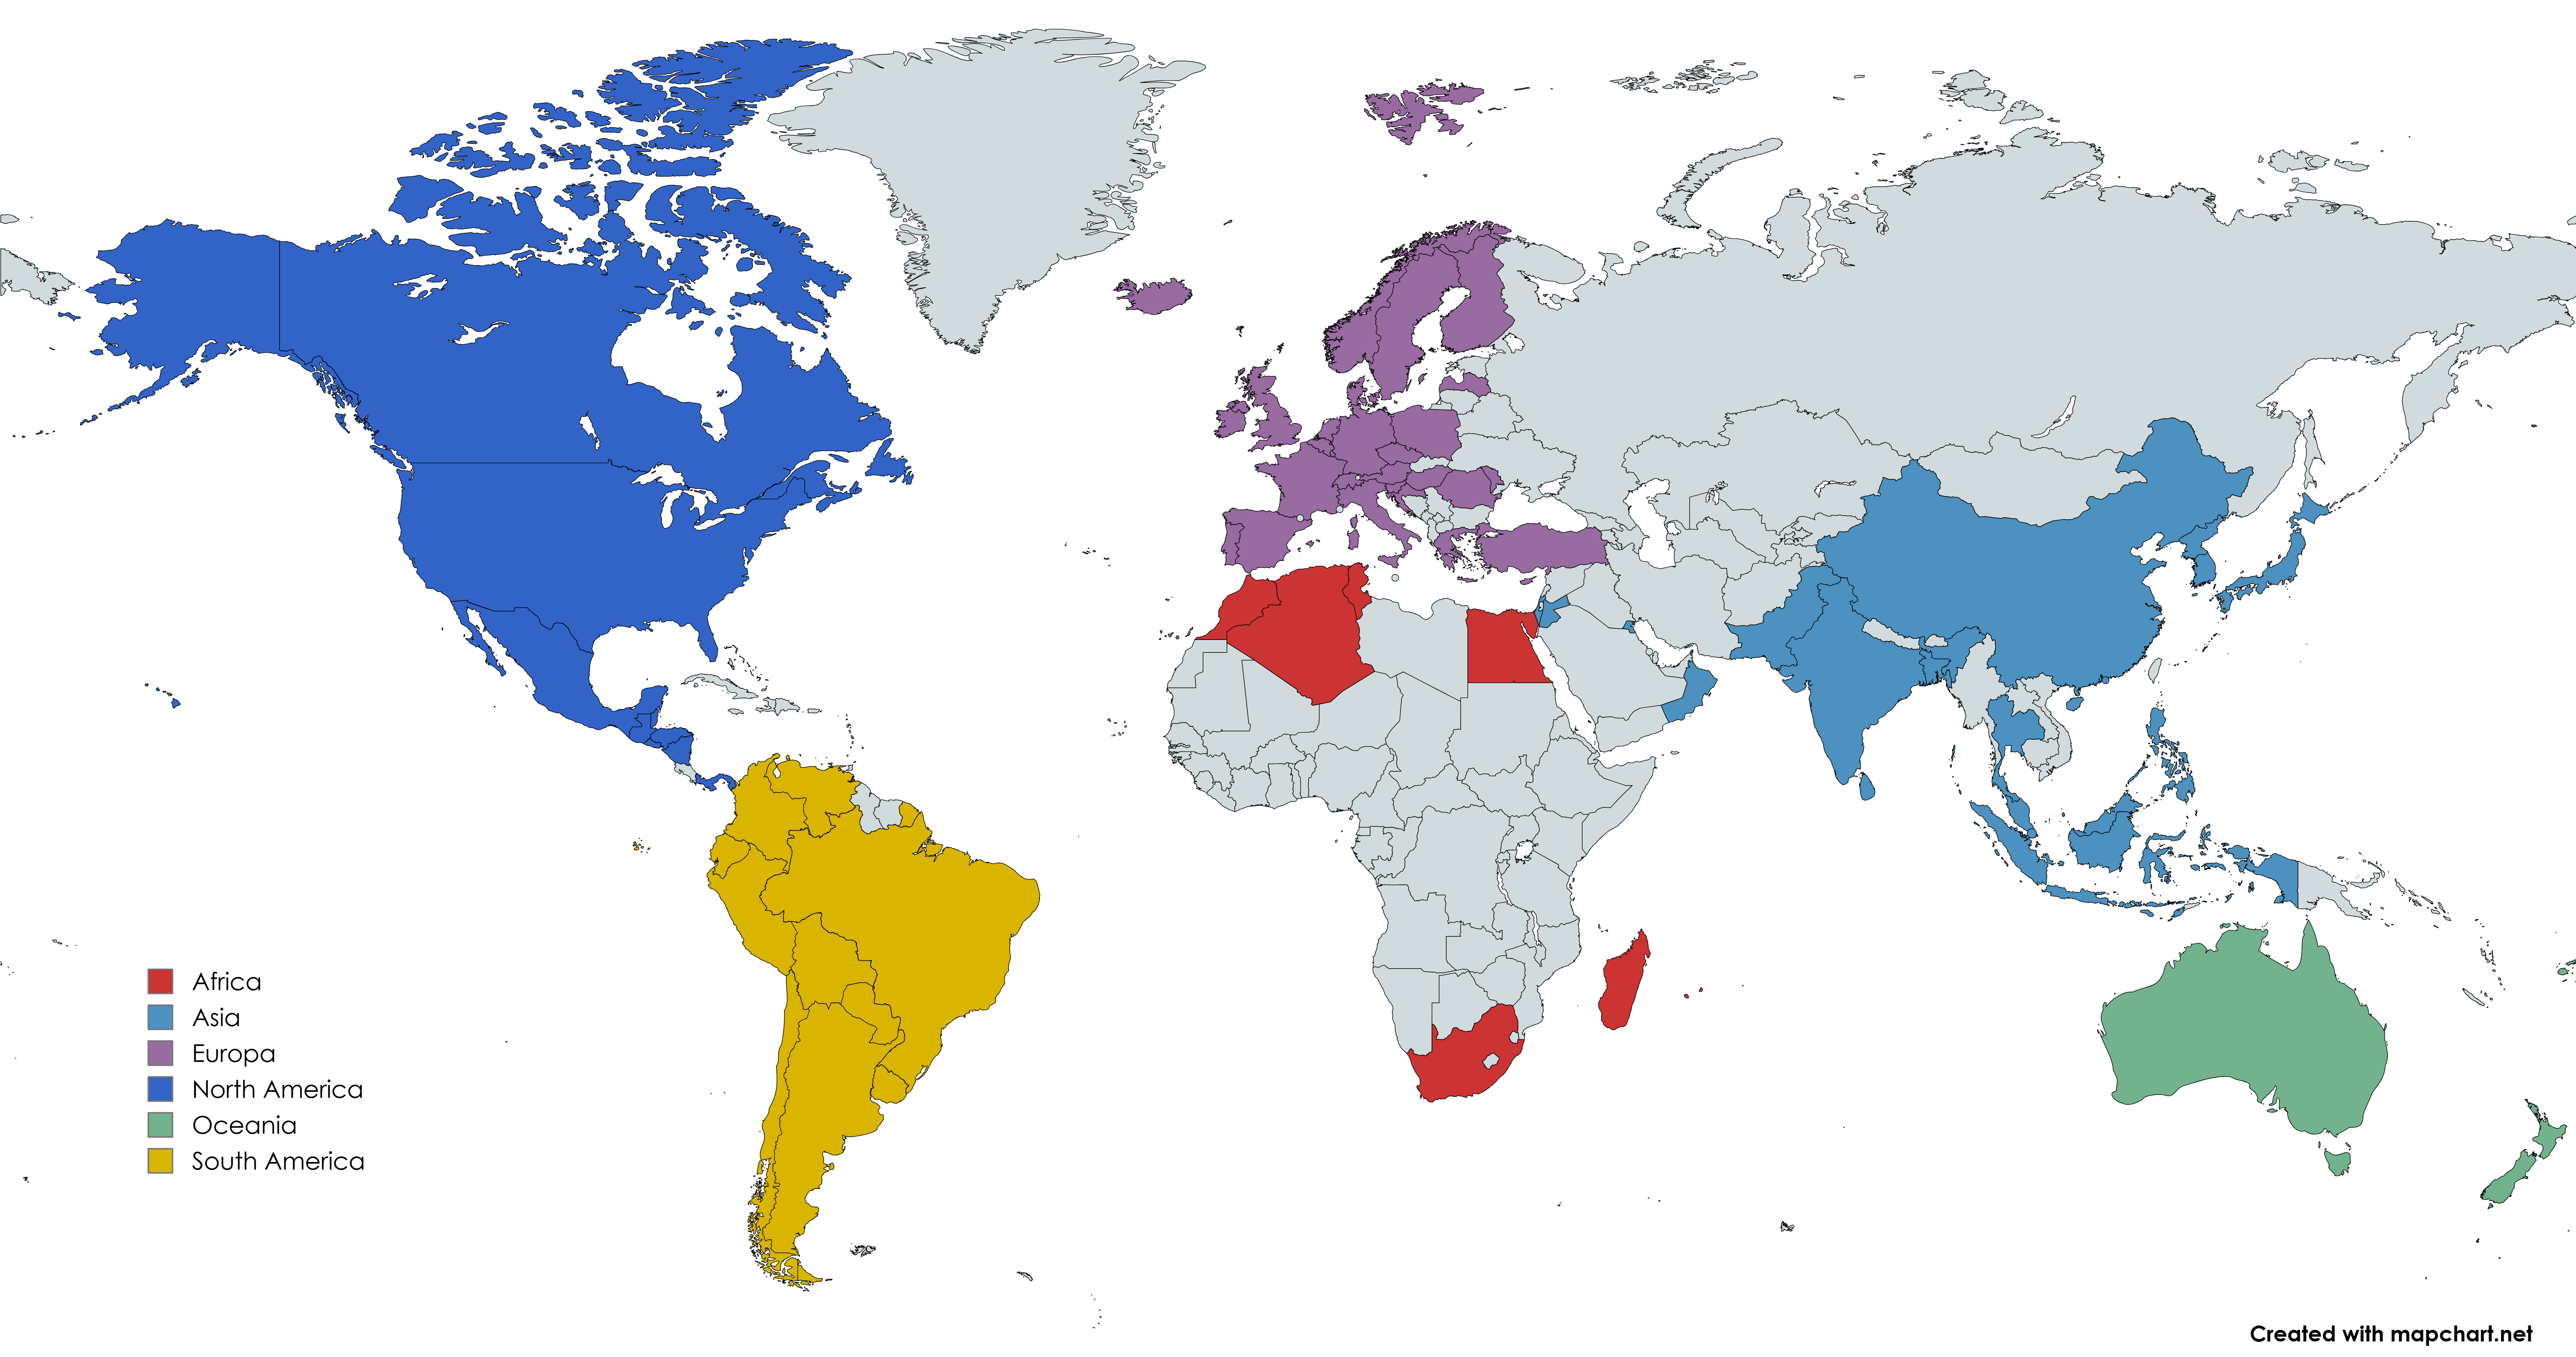
\includegraphics{images/MapChart_Map.png}

Questa è una rappresentazione dei nostri 80 paesi divisi in base
all'attributo ``Continent'' secondo i nostri dati.

    \section{Statistiche di Rete}\label{statistiche-di-rete}

Dopodichè tramite l'utilizzo dei seguenti comandi abbiamo calcolato le
nostre statistiche di Rete.

    \begin{tcolorbox}[breakable, size=fbox, boxrule=1pt, pad at break*=1mm,colback=cellbackground, colframe=cellborder]
\prompt{In}{incolor}{3}{\boxspacing}
\begin{Verbatim}[commandchars=\\\{\}]
\PY{c+c1}{\PYZsh{} Creazione della matrice di adiacenza relativa al grafo g}
\PY{n}{Y}\PY{+w}{ }\PY{o}{\PYZlt{}\PYZhy{}}\PY{+w}{ }\PY{n+nf}{as\PYZus{}adjacency\PYZus{}matrix}\PY{p}{(}\PY{n}{g}\PY{p}{)}
\PY{n+nf}{diag}\PY{p}{(}\PY{n}{Y}\PY{p}{)}\PY{+w}{ }\PY{o}{\PYZlt{}\PYZhy{}}\PY{+w}{ }\PY{k+kc}{NA}

\PY{c+c1}{\PYZsh{} Calcolo delle statistiche di rete}
\PY{n}{rho}\PY{+w}{ }\PY{o}{\PYZlt{}\PYZhy{}}\PY{+w}{ }\PY{n+nf}{edge\PYZus{}density}\PY{p}{(}\PY{n}{g}\PY{p}{)}
\PY{n}{reciprocity}\PY{+w}{ }\PY{o}{\PYZlt{}\PYZhy{}}\PY{+w}{ }\PY{n+nf}{reciprocity}\PY{p}{(}\PY{n}{g}\PY{p}{)}
\PY{n}{transitivity}\PY{+w}{ }\PY{o}{\PYZlt{}\PYZhy{}}\PY{+w}{ }\PY{n+nf}{transitivity}\PY{p}{(}\PY{n}{g}\PY{p}{)}
\PY{n}{odd\PYZus{}rho}\PY{+w}{ }\PY{o}{\PYZlt{}\PYZhy{}}\PY{+w}{ }\PY{n}{rho}\PY{+w}{ }\PY{o}{/}\PY{+w}{ }\PY{p}{(}\PY{l+m}{1}\PY{+w}{ }\PY{o}{\PYZhy{}}\PY{+w}{ }\PY{n}{rho}\PY{p}{)}
\PY{n}{odd\PYZus{}transitivity}\PY{+w}{ }\PY{o}{\PYZlt{}\PYZhy{}}\PY{+w}{ }\PY{n}{transitivity}\PY{+w}{ }\PY{o}{/}\PY{+w}{ }\PY{p}{(}\PY{l+m}{1}\PY{+w}{ }\PY{o}{\PYZhy{}}\PY{+w}{ }\PY{n}{transitivity}\PY{p}{)}
\PY{n}{tau}\PY{+w}{ }\PY{o}{\PYZlt{}\PYZhy{}}\PY{+w}{ }\PY{n}{odd\PYZus{}transitivity}\PY{+w}{ }\PY{o}{/}\PY{+w}{ }\PY{n}{odd\PYZus{}rho}
\PY{n}{assortativity\PYZus{}continent}\PY{+w}{ }\PY{o}{\PYZlt{}\PYZhy{}}\PY{+w}{ }\PY{n+nf}{assortativity}\PY{p}{(}\PY{n}{g}\PY{p}{,}\PY{+w}{ }\PY{n+nf}{V}\PY{p}{(}\PY{n}{g}\PY{p}{)}\PY{o}{\PYZdl{}}\PY{n}{continent}\PY{p}{,}\PY{+w}{ }\PY{n}{directed}\PY{+w}{ }\PY{o}{=}\PY{+w}{ }\PY{k+kc}{TRUE}\PY{p}{)}
\PY{n}{assortativity\PYZus{}gdp}\PY{+w}{ }\PY{o}{\PYZlt{}\PYZhy{}}\PY{+w}{ }\PY{n+nf}{assortativity}\PY{p}{(}\PY{n}{g}\PY{p}{,}\PY{+w}{ }\PY{n+nf}{V}\PY{p}{(}\PY{n}{g}\PY{p}{)}\PY{o}{\PYZdl{}}\PY{n}{gdp}\PY{p}{,}\PY{+w}{ }\PY{n}{directed}\PY{+w}{ }\PY{o}{=}\PY{+w}{ }\PY{k+kc}{TRUE}\PY{p}{)}
\PY{n}{assortativity\PYZus{}worldpartition}\PY{+w}{ }\PY{o}{\PYZlt{}\PYZhy{}}\PY{+w}{ }\PY{n+nf}{assortativity}\PY{p}{(}\PY{n}{g}\PY{p}{,}\PY{+w}{ }\PY{n+nf}{V}\PY{p}{(}\PY{n}{g}\PY{p}{)}\PY{o}{\PYZdl{}}\PY{n}{world\PYZus{}partition}\PY{p}{,}\PY{+w}{ }\PY{n}{directed}\PY{+w}{ }\PY{o}{=}\PY{+w}{ }\PY{k+kc}{TRUE}\PY{p}{)}

\PY{c+c1}{\PYZsh{} Create a table with names and values}
\PY{n}{table}\PY{+w}{ }\PY{o}{\PYZlt{}\PYZhy{}}\PY{+w}{ }\PY{n+nf}{data.frame}\PY{p}{(}
\PY{+w}{	}\PY{n}{Name}\PY{+w}{ }\PY{o}{=}\PY{+w}{ }\PY{n+nf}{c}\PY{p}{(}\PY{l+s}{\PYZdq{}}\PY{l+s}{Edge Density\PYZdq{}}\PY{p}{,}\PY{+w}{ }\PY{l+s}{\PYZdq{}}\PY{l+s}{Reciprocity\PYZdq{}}\PY{p}{,}\PY{+w}{ }\PY{l+s}{\PYZdq{}}\PY{l+s}{Transitivity\PYZdq{}}\PY{p}{,}\PY{+w}{ }\PY{l+s}{\PYZdq{}}\PY{l+s}{Tau\PYZdq{}}\PY{p}{,}\PY{+w}{ }\PY{l+s}{\PYZdq{}}\PY{l+s}{Assortativity (Continent)\PYZdq{}}\PY{p}{,}\PY{+w}{ }\PY{l+s}{\PYZdq{}}\PY{l+s}{Assortativity (GDP)\PYZdq{}}\PY{p}{,}\PY{+w}{ }\PY{l+s}{\PYZdq{}}\PY{l+s}{Assortativity (World Partition)\PYZdq{}}\PY{p}{)}\PY{p}{,}
\PY{+w}{	}\PY{n}{Value}\PY{+w}{ }\PY{o}{=}\PY{+w}{ }\PY{n+nf}{c}\PY{p}{(}\PY{n}{rho}\PY{p}{,}\PY{+w}{ }\PY{n}{reciprocity}\PY{p}{,}\PY{+w}{ }\PY{n}{transitivity}\PY{p}{,}\PY{+w}{ }\PY{n}{tau}\PY{p}{,}\PY{+w}{ }\PY{n}{assortativity\PYZus{}continent}\PY{p}{,}\PY{+w}{ }\PY{n}{assortativity\PYZus{}gdp}\PY{p}{,}\PY{+w}{ }\PY{n}{assortativity\PYZus{}worldpartition}\PY{p}{)}
\PY{p}{)}

\PY{n+nf}{createImageFromTable}\PY{p}{(}\PY{n}{table}\PY{p}{,}\PY{+w}{ }\PY{n}{filename}\PY{+w}{ }\PY{o}{=}\PY{+w}{ }\PY{l+s}{\PYZdq{}}\PY{l+s}{images/NetworkStatisticsTable.png\PYZdq{}}\PY{p}{,}\PY{+w}{ }\PY{n}{width}\PY{+w}{ }\PY{o}{=}\PY{+w}{ }\PY{l+m}{1500}\PY{p}{,}\PY{+w}{ }\PY{n}{height}\PY{+w}{ }\PY{o}{=}\PY{+w}{ }\PY{l+m}{1050}\PY{p}{,}\PY{+w}{ }\PY{n}{res}\PY{+w}{ }\PY{o}{=}\PY{+w}{ }\PY{l+m}{440}\PY{p}{)}
\end{Verbatim}
\end{tcolorbox}

    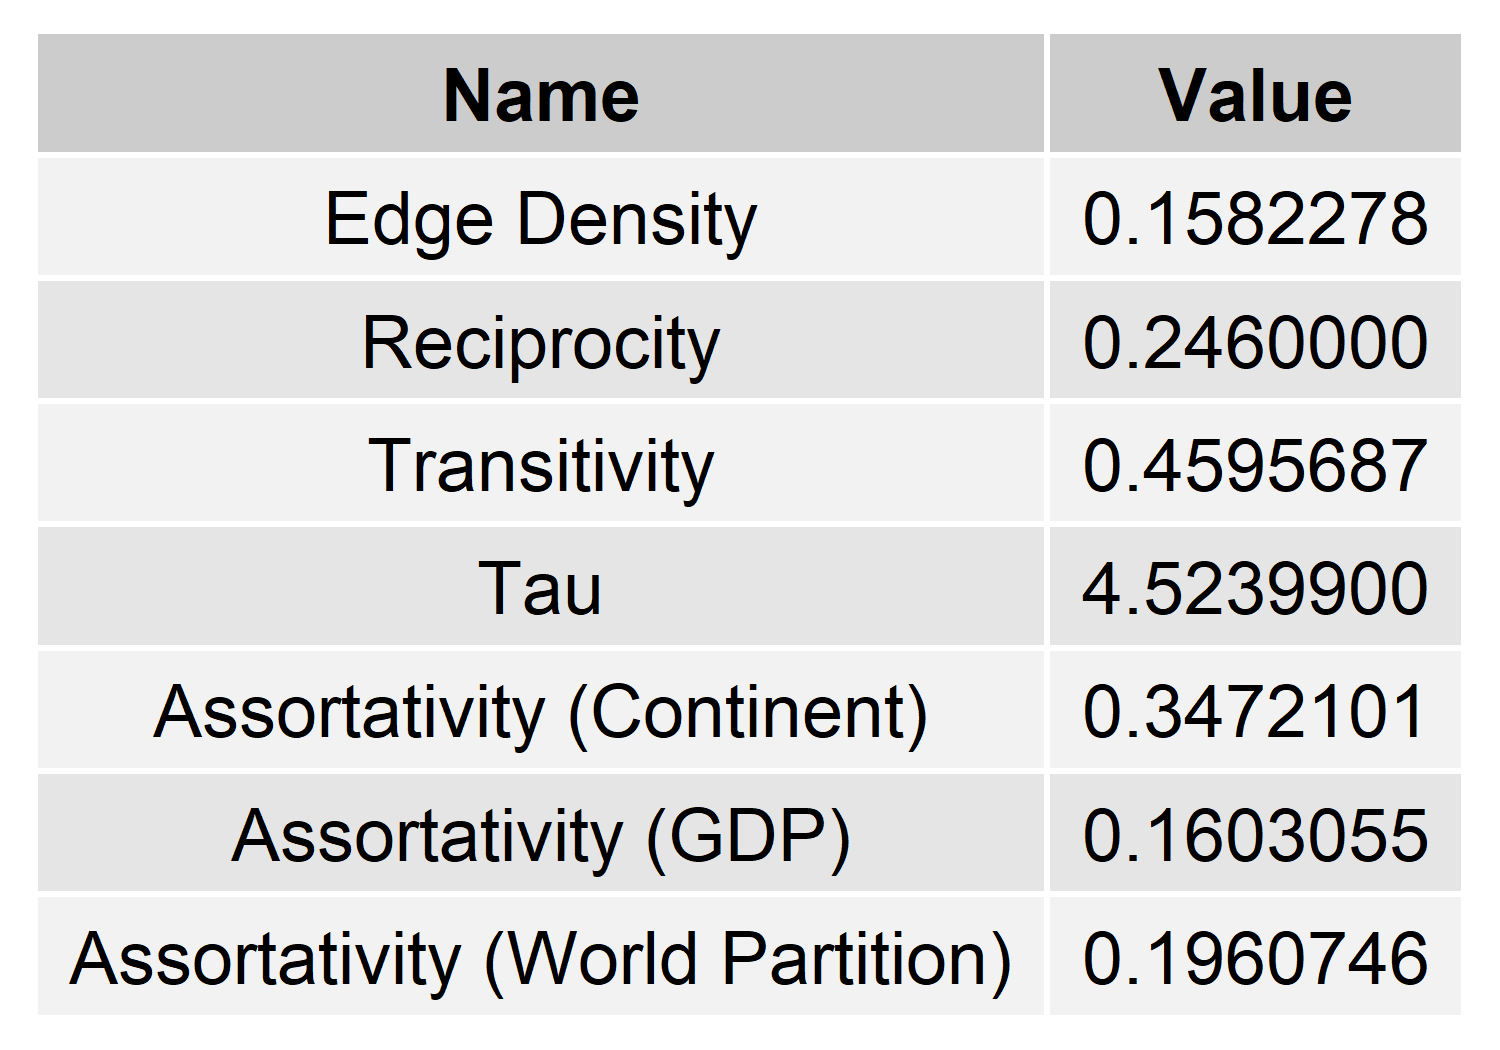
\includegraphics{images/NetworkStatisticsTable.png}

Tabella delle Statistiche di Rete

    Dall'immagine sopra possiamo estrapolare delle informazioni riguardo
alla nostra rete, cioè:

\begin{itemize}
\tightlist
\item
  Circa 1/4 delle connessioni è reciprocata.
\item
  La transitività nella nostra rete è molto alta, circa 4 volte di più
  rispetto al caso random.
\item
  Il coefficiente di assortatività è positivo per tutti e 3 gli
  attributi nodali.
\end{itemize}

Con queste informazioni possiamo già dire che la nostra rete ha un'alta
tendenza a formare dei cluster (o gruppi).

    \section{Statistiche Nodali}\label{statistiche-nodali}

Per quanto riguarda le Statistiche Nodali, cioè:

\begin{itemize}
\tightlist
\item
  Degree Centrality
\item
  Closeness Centrality
\item
  Betweenness Centrality
\item
  Eigen-Vector Centrality
\end{itemize}

abbiamo ottenuto i seguenti risultati:

    \subsection{Degree Centrality}\label{degree-centrality}

    Nel nostro caso la Degree Centrality può essere interpretata come un
valore che indica se un paese effettua dei commerci relativi agli
oggetti in metallo oppure no.

Essendo la nostra rete una rete direzionata, dobbiamo osservare sia la
In-Degree Centrality che la Out-Degree Centrality.

    \begin{tcolorbox}[breakable, size=fbox, boxrule=1pt, pad at break*=1mm,colback=cellbackground, colframe=cellborder]
\prompt{In}{incolor}{4}{\boxspacing}
\begin{Verbatim}[commandchars=\\\{\}]
\PY{n}{in\PYZus{}degree}\PY{+w}{ }\PY{o}{\PYZlt{}\PYZhy{}}\PY{+w}{ }\PY{n+nf}{degree}\PY{p}{(}\PY{n}{g}\PY{p}{,}\PY{+w}{ }\PY{n}{mode}\PY{+w}{ }\PY{o}{=}\PY{+w}{ }\PY{l+s}{\PYZdq{}}\PY{l+s}{in\PYZdq{}}\PY{p}{)}
\PY{n}{out\PYZus{}degree}\PY{+w}{ }\PY{o}{\PYZlt{}\PYZhy{}}\PY{+w}{ }\PY{n+nf}{degree}\PY{p}{(}\PY{n}{g}\PY{p}{,}\PY{+w}{ }\PY{n}{mode}\PY{+w}{ }\PY{o}{=}\PY{+w}{ }\PY{l+s}{\PYZdq{}}\PY{l+s}{out\PYZdq{}}\PY{p}{)}
\end{Verbatim}
\end{tcolorbox}

    \subsubsection{In-Degree Centrality}\label{in-degree-centrality}

I dati da noi ottenuti per la In-Degree Centrality sono i seguenti:

    \begin{tcolorbox}[breakable, size=fbox, boxrule=1pt, pad at break*=1mm,colback=cellbackground, colframe=cellborder]
\prompt{In}{incolor}{5}{\boxspacing}
\begin{Verbatim}[commandchars=\\\{\}]
\PY{c+c1}{\PYZsh{} Istogramma dell\PYZsq{}In Degree Centrality}
\PY{n+nf}{hist}\PY{p}{(}\PY{n}{in\PYZus{}degree}\PY{p}{)}
\end{Verbatim}
\end{tcolorbox}

    \begin{center}
    \adjustimage{max size={0.9\linewidth}{0.9\paperheight}}{relazioneProgetto_files/relazioneProgetto_17_0.png}
    \end{center}
    { \hspace*{\fill} \\}
    
    \begin{tcolorbox}[breakable, size=fbox, boxrule=1pt, pad at break*=1mm,colback=cellbackground, colframe=cellborder]
\prompt{In}{incolor}{6}{\boxspacing}
\begin{Verbatim}[commandchars=\\\{\}]
\PY{c+c1}{\PYZsh{} Stampo il Summary dell\PYZsq{}In Degree Centrality}
\PY{n+nf}{summary}\PY{p}{(}\PY{n}{in\PYZus{}degree}\PY{p}{)}
\end{Verbatim}
\end{tcolorbox}

    
    \begin{Verbatim}[commandchars=\\\{\}]
   Min. 1st Qu.  Median    Mean 3rd Qu.    Max. 
    4.0    10.0    13.0    12.5    15.0    18.0 
    \end{Verbatim}

    
    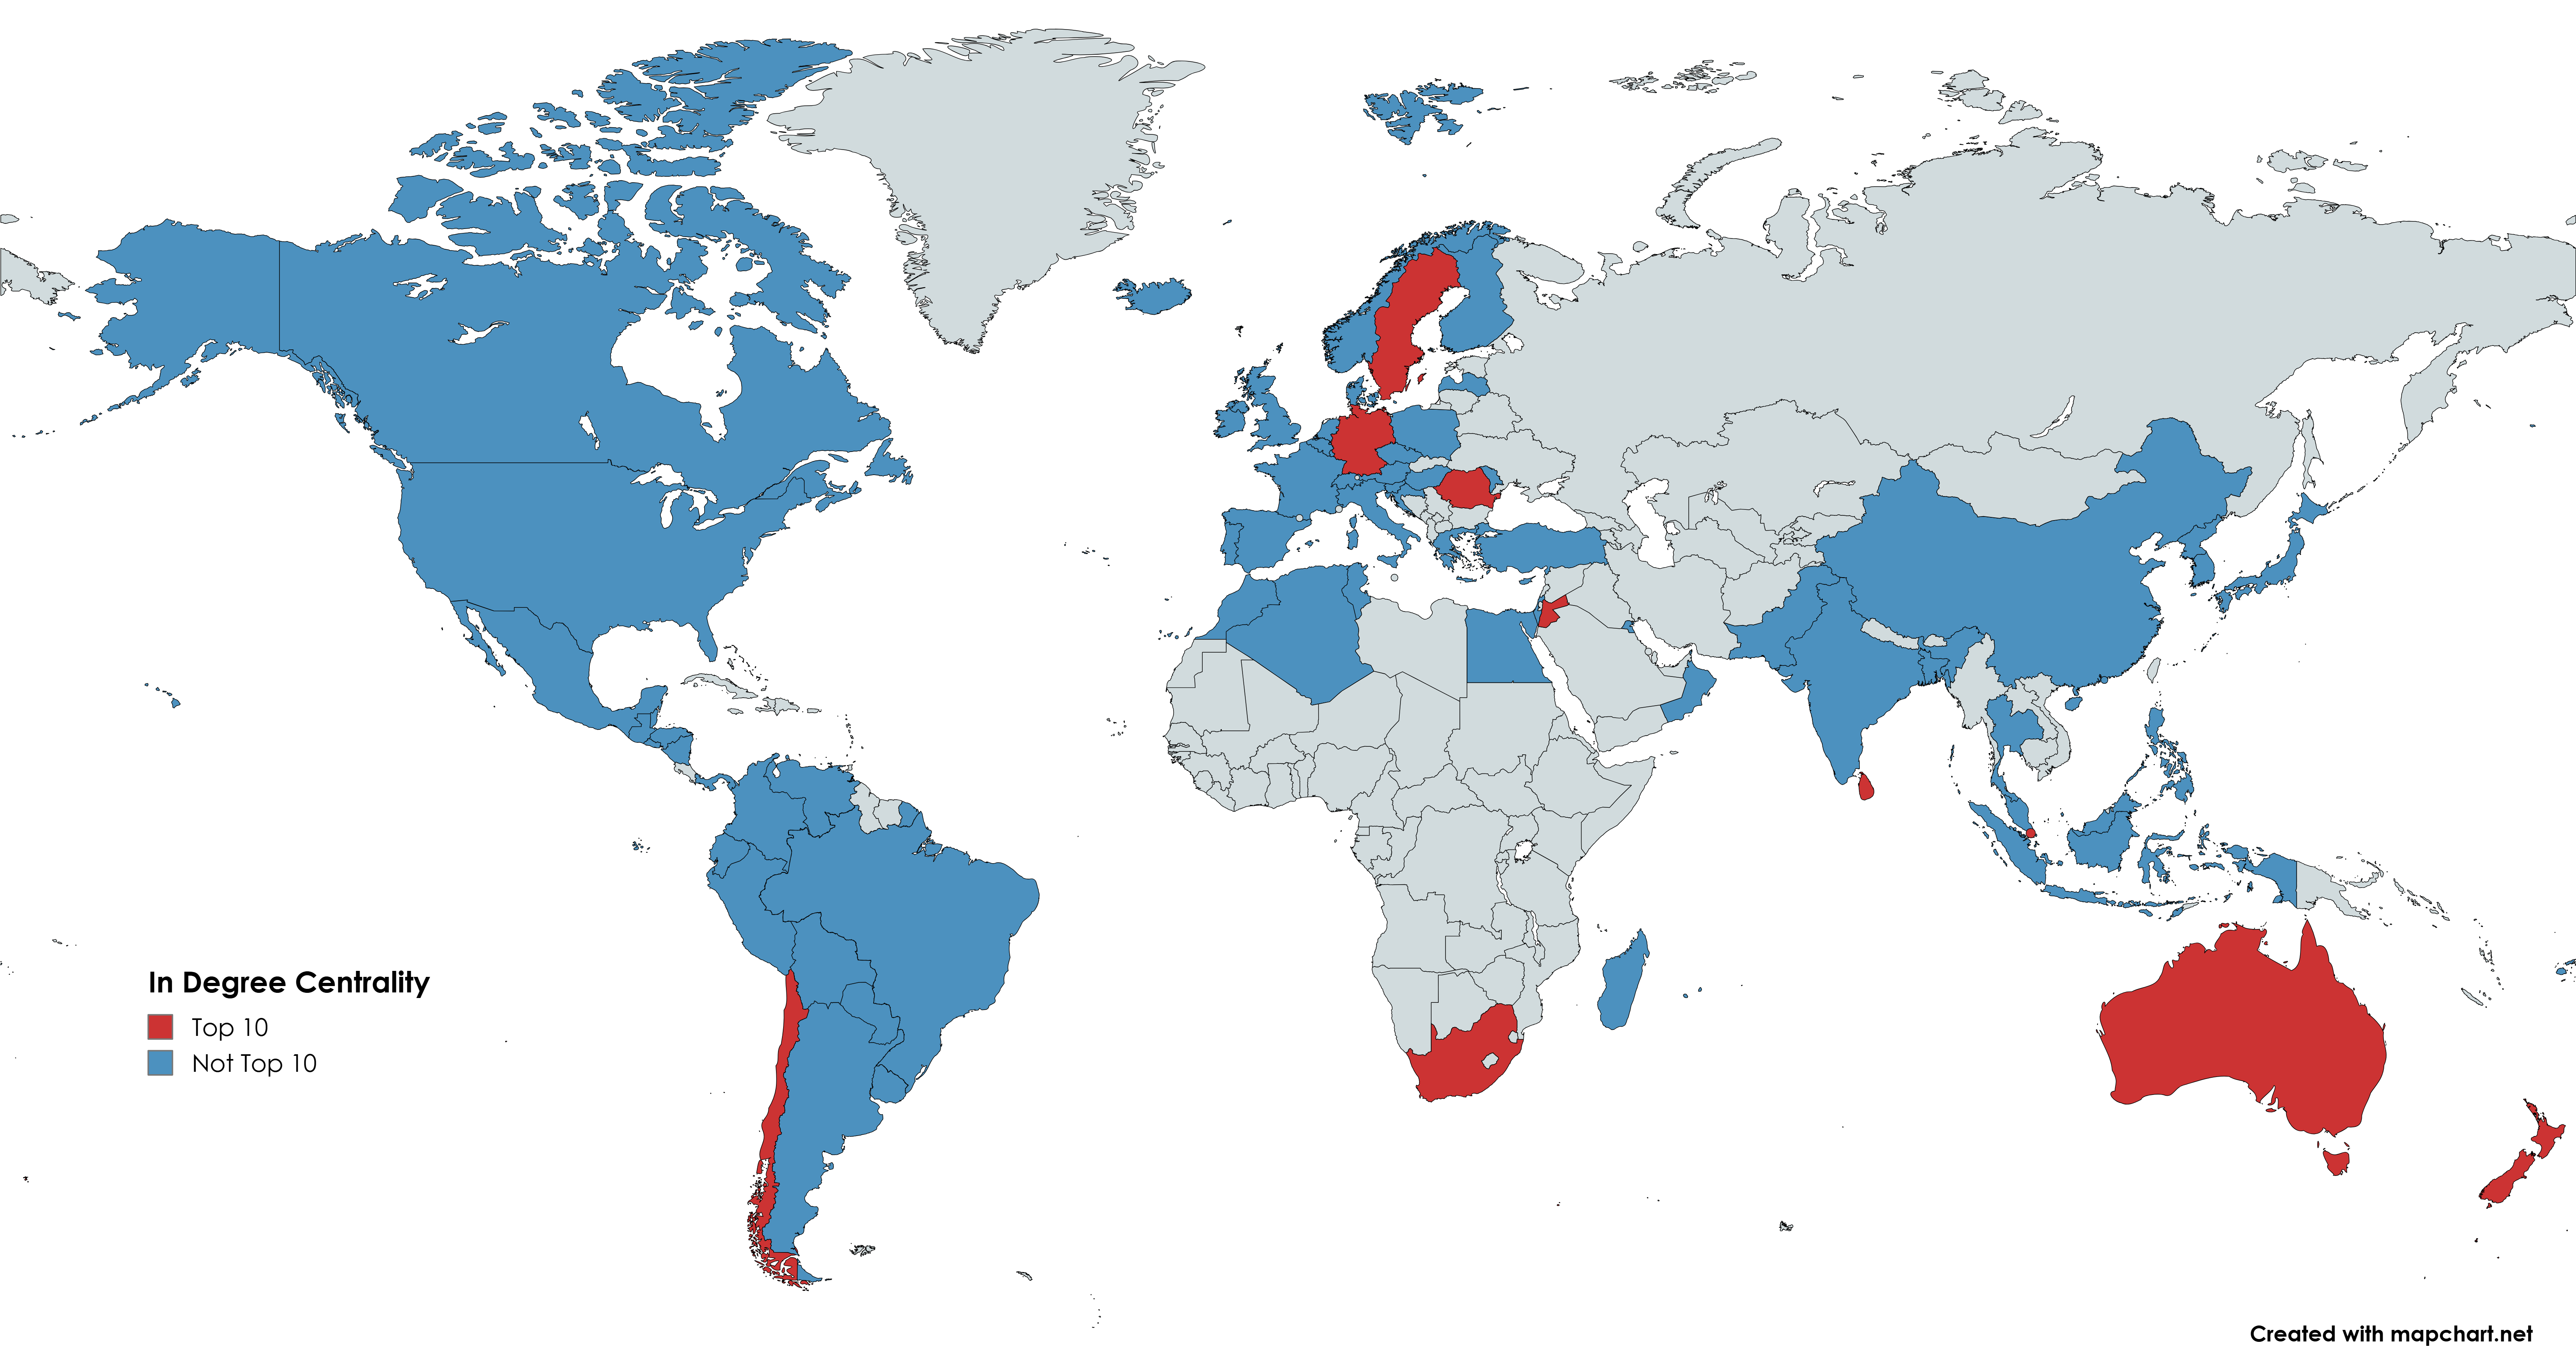
\includegraphics{imagesWorldMaps/In_Degree_Centrality.png}

Top 10 Nazioni rispetto all'In Degree

    \begin{tcolorbox}[breakable, size=fbox, boxrule=1pt, pad at break*=1mm,colback=cellbackground, colframe=cellborder]
\prompt{In}{incolor}{7}{\boxspacing}
\begin{Verbatim}[commandchars=\\\{\}]
\PY{c+c1}{\PYZsh{} Stampo la centralità della Rete rispetto all\PYZsq{}In Degree}
\PY{n+nf}{centr\PYZus{}degree}\PY{p}{(}\PY{n}{g}\PY{p}{,}\PY{+w}{ }\PY{n}{loops}\PY{+w}{ }\PY{o}{=}\PY{+w}{ }\PY{k+kc}{FALSE}\PY{p}{,}\PY{+w}{ }\PY{n}{mode}\PY{+w}{ }\PY{o}{=}\PY{+w}{ }\PY{l+s}{\PYZdq{}}\PY{l+s}{in\PYZdq{}}\PY{p}{)}\PY{o}{\PYZdl{}}\PY{n}{centralization}
\end{Verbatim}
\end{tcolorbox}

    0.0705015221919564

    
    \paragraph{Conclusioni}\label{conclusioni}

    Come possiamo vedere dall'istogramma e dal valore di centralizzazione,
tutti i paesi esportano metalli, e non ci sono paesi che esportano in
maniera molto più marcata rispetto ad altri

    \subsubsection{Out-Degree Centrality}\label{out-degree-centrality}

Invece per quanto riguarda la Out-Degree Centrality abbiamo ottenuto i
seguenti risultati:

    \begin{tcolorbox}[breakable, size=fbox, boxrule=1pt, pad at break*=1mm,colback=cellbackground, colframe=cellborder]
\prompt{In}{incolor}{8}{\boxspacing}
\begin{Verbatim}[commandchars=\\\{\}]
\PY{c+c1}{\PYZsh{} Istogramma dell\PYZsq{}In Degree Centrality}
\PY{n+nf}{hist}\PY{p}{(}\PY{n}{out\PYZus{}degree}\PY{p}{,}\PY{+w}{ }\PY{n}{breaks}\PY{+w}{ }\PY{o}{=}\PY{+w}{ }\PY{l+m}{10}\PY{p}{)}
\end{Verbatim}
\end{tcolorbox}

    \begin{center}
    \adjustimage{max size={0.9\linewidth}{0.9\paperheight}}{relazioneProgetto_files/relazioneProgetto_24_0.png}
    \end{center}
    { \hspace*{\fill} \\}
    
    \begin{tcolorbox}[breakable, size=fbox, boxrule=1pt, pad at break*=1mm,colback=cellbackground, colframe=cellborder]
\prompt{In}{incolor}{9}{\boxspacing}
\begin{Verbatim}[commandchars=\\\{\}]
\PY{c+c1}{\PYZsh{} Stampo il Summary dell\PYZsq{}In Degree Centrality}
\PY{n+nf}{summary}\PY{p}{(}\PY{n}{out\PYZus{}degree}\PY{p}{)}
\end{Verbatim}
\end{tcolorbox}

    
    \begin{Verbatim}[commandchars=\\\{\}]
   Min. 1st Qu.  Median    Mean 3rd Qu.    Max. 
    0.0     0.0     4.0    12.5    13.0    77.0 
    \end{Verbatim}

    
    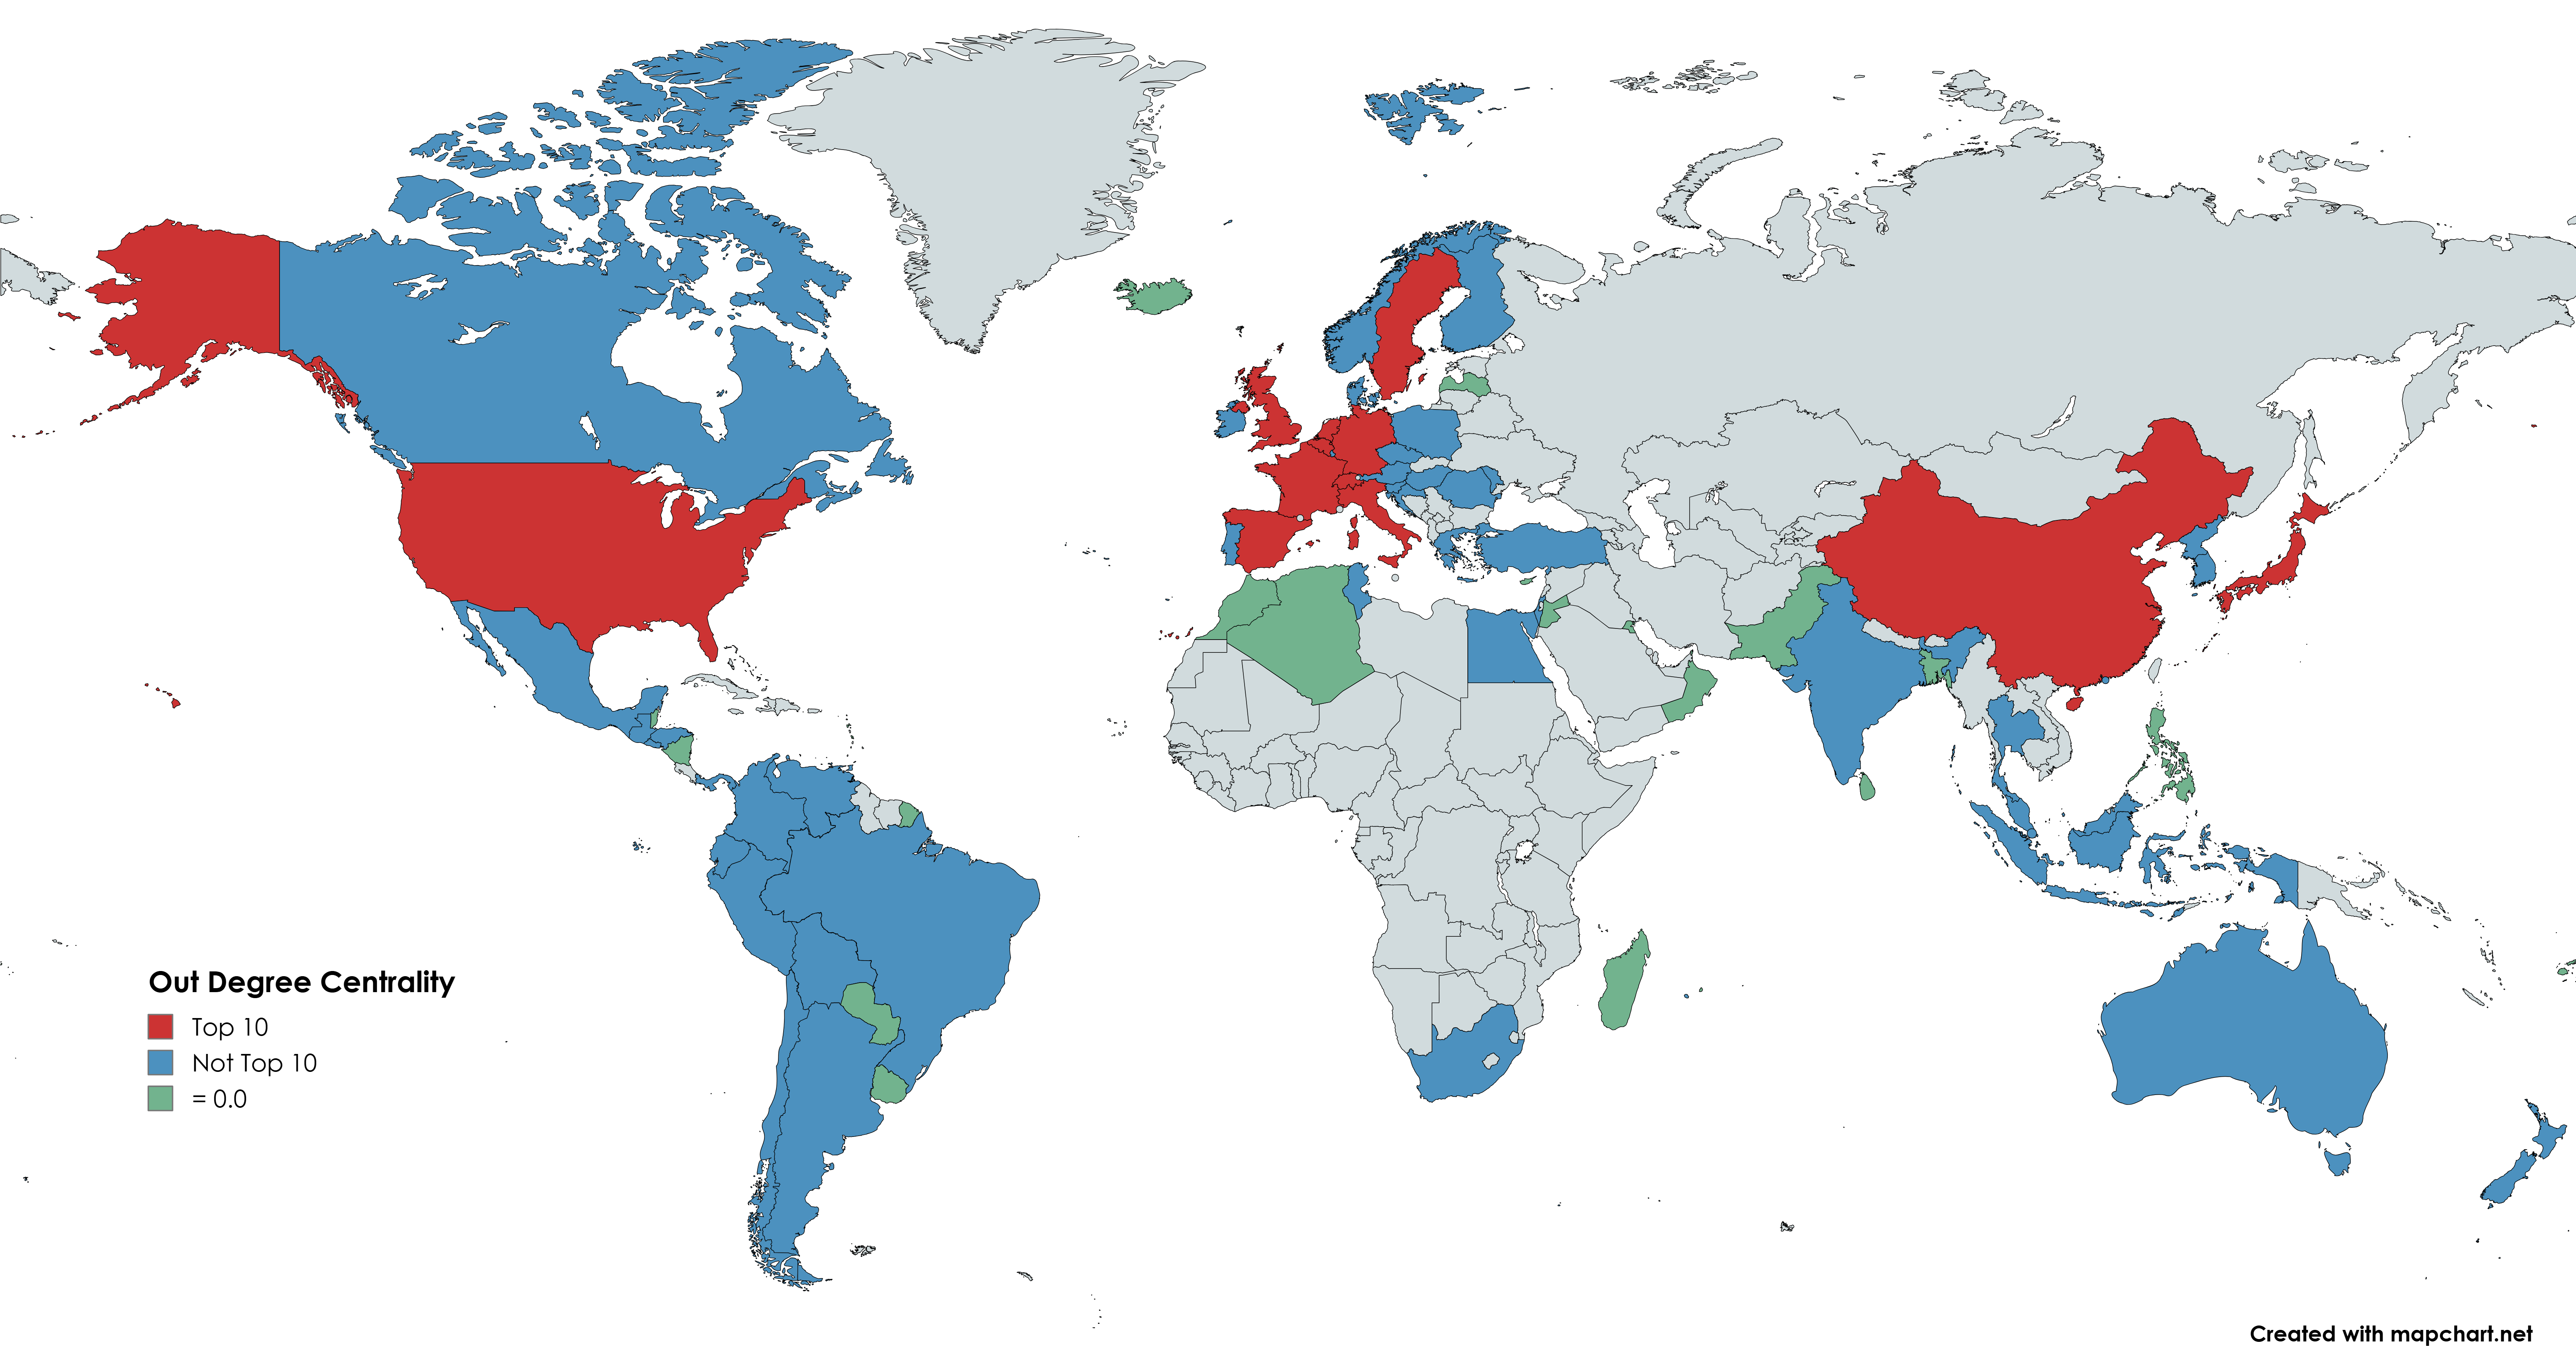
\includegraphics{imagesWorldMaps/Out_Degree_Centrality.png}

Top 10 Nazioni rispetto all'Out Degree

    \begin{tcolorbox}[breakable, size=fbox, boxrule=1pt, pad at break*=1mm,colback=cellbackground, colframe=cellborder]
\prompt{In}{incolor}{10}{\boxspacing}
\begin{Verbatim}[commandchars=\\\{\}]
\PY{c+c1}{\PYZsh{} Stampo la centralità della Rete rispetto all\PYZsq{}In Degree}
\PY{n+nf}{centr\PYZus{}degree}\PY{p}{(}\PY{n}{g}\PY{p}{,}\PY{+w}{ }\PY{n}{loops}\PY{+w}{ }\PY{o}{=}\PY{+w}{ }\PY{k+kc}{FALSE}\PY{p}{,}\PY{+w}{ }\PY{n}{mode}\PY{+w}{ }\PY{o}{=}\PY{+w}{ }\PY{l+s}{\PYZdq{}}\PY{l+s}{out\PYZdq{}}\PY{p}{)}\PY{o}{\PYZdl{}}\PY{n}{centralization}
\end{Verbatim}
\end{tcolorbox}

    0.826790578432943

    
    \paragraph{Conclusioni}\label{conclusioni}

    Stavolta, visualizzando l'istogramma e il valore di centralizzazione
possiamo vedere come ci siano alcuni nodi che sono molto più centrali di
altri. Dal grafico riportato sopra possiamo concludere che questi sono i
paesi più sviluppati (Stati Uniti, paesi europei e Cina)

    \subsection{Closeness Centrality}\label{closeness-centrality}

Nel nostro caso non siamo riusciti a trovare un `senso' alla Closeness
Centrality, abbiamo comunque deciso di studiarla perchè forse potrebbe
risultare qualche informazione interessante.

Essendo la nostra rete una rete direzionata, dobbiamo osservare sia la
In-Closeness Centrality che la Out-Closeness Centrality.

    \begin{tcolorbox}[breakable, size=fbox, boxrule=1pt, pad at break*=1mm,colback=cellbackground, colframe=cellborder]
\prompt{In}{incolor}{11}{\boxspacing}
\begin{Verbatim}[commandchars=\\\{\}]
\PY{n}{closeness\PYZus{}in}\PY{+w}{ }\PY{o}{\PYZlt{}\PYZhy{}}\PY{+w}{ }\PY{n+nf}{closeness}\PY{p}{(}\PY{n}{g}\PY{p}{,}\PY{+w}{ }\PY{n}{mode}\PY{+w}{ }\PY{o}{=}\PY{+w}{ }\PY{l+s}{\PYZdq{}}\PY{l+s}{in\PYZdq{}}\PY{p}{)}
\PY{n}{closeness\PYZus{}out}\PY{+w}{ }\PY{o}{\PYZlt{}\PYZhy{}}\PY{+w}{ }\PY{n+nf}{closeness}\PY{p}{(}\PY{n}{g}\PY{p}{,}\PY{+w}{ }\PY{n}{mode}\PY{+w}{ }\PY{o}{=}\PY{+w}{ }\PY{l+s}{\PYZdq{}}\PY{l+s}{out\PYZdq{}}\PY{p}{)}
\end{Verbatim}
\end{tcolorbox}

    \subsubsection{In-Closeness Centrality}\label{in-closeness-centrality}

I Dati da noi ottenuti per la In-Closeness Centrality sono i seguenti

    \begin{tcolorbox}[breakable, size=fbox, boxrule=1pt, pad at break*=1mm,colback=cellbackground, colframe=cellborder]
\prompt{In}{incolor}{12}{\boxspacing}
\begin{Verbatim}[commandchars=\\\{\}]
\PY{c+c1}{\PYZsh{}Istogramma dell\PYZsq{}In\PYZhy{}Closeness Centrality}
\PY{n+nf}{hist}\PY{p}{(}\PY{n}{closeness\PYZus{}in}\PY{p}{)}
\end{Verbatim}
\end{tcolorbox}

    \begin{center}
    \adjustimage{max size={0.9\linewidth}{0.9\paperheight}}{relazioneProgetto_files/relazioneProgetto_33_0.png}
    \end{center}
    { \hspace*{\fill} \\}
    
    \begin{tcolorbox}[breakable, size=fbox, boxrule=1pt, pad at break*=1mm,colback=cellbackground, colframe=cellborder]
\prompt{In}{incolor}{13}{\boxspacing}
\begin{Verbatim}[commandchars=\\\{\}]
\PY{n+nf}{summary}\PY{p}{(}\PY{n}{closeness\PYZus{}in}\PY{p}{)}
\end{Verbatim}
\end{tcolorbox}

    
    \begin{Verbatim}[commandchars=\\\{\}]
    Min.  1st Qu.   Median     Mean  3rd Qu.     Max. 
0.005848 0.006623 0.006944 0.007488 0.007634 0.011364 
    \end{Verbatim}

    
    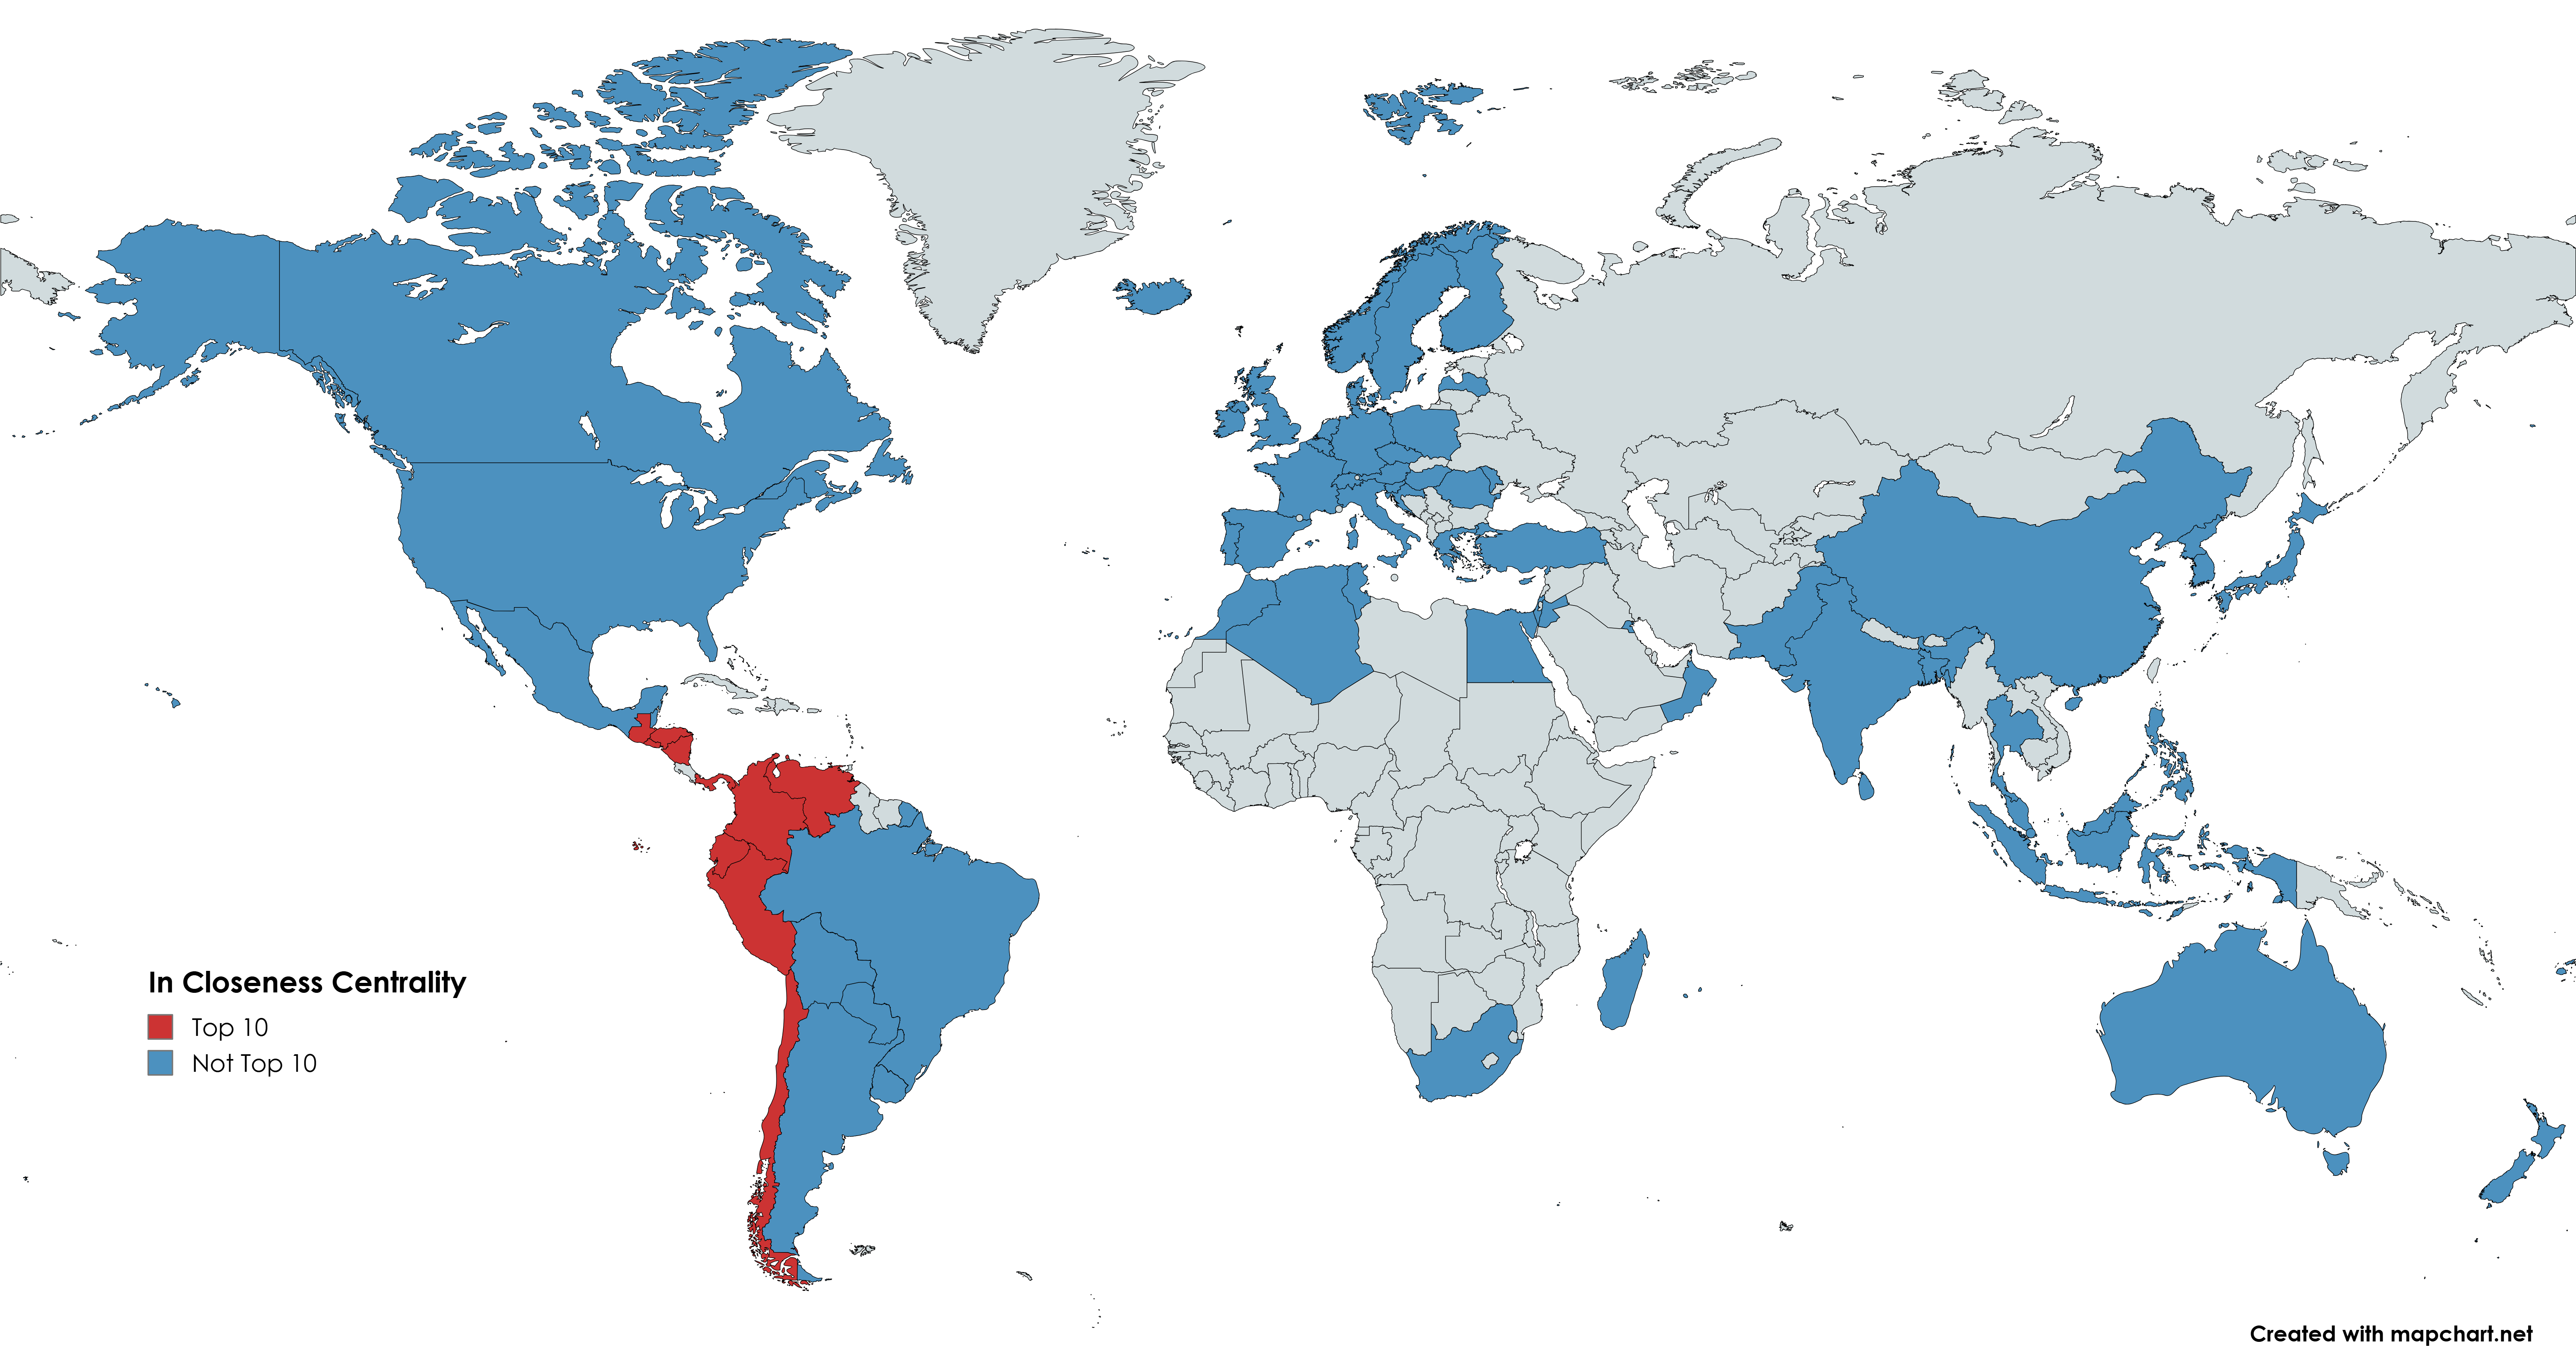
\includegraphics{imagesWorldMaps/In_Closeness_Centrality.png}

Top 10 Nazioni rispetto all'In Closeness

    \begin{tcolorbox}[breakable, size=fbox, boxrule=1pt, pad at break*=1mm,colback=cellbackground, colframe=cellborder]
\prompt{In}{incolor}{14}{\boxspacing}
\begin{Verbatim}[commandchars=\\\{\}]
\PY{n+nf}{centr\PYZus{}clo}\PY{p}{(}\PY{n}{g}\PY{p}{,}\PY{+w}{ }\PY{n}{mode}\PY{+w}{ }\PY{o}{=}\PY{+w}{ }\PY{l+s}{\PYZdq{}}\PY{l+s}{in\PYZdq{}}\PY{p}{)}\PY{o}{\PYZdl{}}\PY{n}{centralization}
\end{Verbatim}
\end{tcolorbox}

    0.17667852352639

    
    \paragraph{Conclusioni}\label{conclusioni}

\begin{itemize}
\tightlist
\item
  Nella rete non sono presenti nodi con In Closeness infinita, il che
  implica che tutti i nodi sono raggiungibili da ogni altro nodo
\item
  I Paesi con l'In Closeness maggiore sono quasi tutti Paesi
  dell'America del Sud (questa informazione potrebbe essere interessante
  da studiare, ma non essendo oggetto della nostra relazione non abbiamo
  approfondito oltre)
\end{itemize}

    \subsubsection{Out-Closeness Centrality}\label{out-closeness-centrality}

I Dati da noi ottenuti per la In-Closeness Centrality sono i seguenti

    \begin{tcolorbox}[breakable, size=fbox, boxrule=1pt, pad at break*=1mm,colback=cellbackground, colframe=cellborder]
\prompt{In}{incolor}{15}{\boxspacing}
\begin{Verbatim}[commandchars=\\\{\}]
\PY{c+c1}{\PYZsh{}Istogramma dell\PYZsq{}Out\PYZhy{}Closeness Centrality}
\PY{n+nf}{hist}\PY{p}{(}\PY{n}{closeness\PYZus{}out}\PY{p}{,}\PY{+w}{ }\PY{n}{breaks}\PY{+w}{ }\PY{o}{=}\PY{+w}{ }\PY{l+m}{20}\PY{p}{)}
\end{Verbatim}
\end{tcolorbox}

    \begin{center}
    \adjustimage{max size={0.9\linewidth}{0.9\paperheight}}{relazioneProgetto_files/relazioneProgetto_39_0.png}
    \end{center}
    { \hspace*{\fill} \\}
    
    \begin{tcolorbox}[breakable, size=fbox, boxrule=1pt, pad at break*=1mm,colback=cellbackground, colframe=cellborder]
\prompt{In}{incolor}{16}{\boxspacing}
\begin{Verbatim}[commandchars=\\\{\}]
\PY{n+nf}{summary}\PY{p}{(}\PY{n}{closeness\PYZus{}out}\PY{p}{)}
\end{Verbatim}
\end{tcolorbox}

    
    \begin{Verbatim}[commandchars=\\\{\}]
    Min.  1st Qu.   Median     Mean  3rd Qu.     Max.     NA's 
0.001435 0.004959 0.006645 0.056027 0.009901 0.500000       24 
    \end{Verbatim}

    
    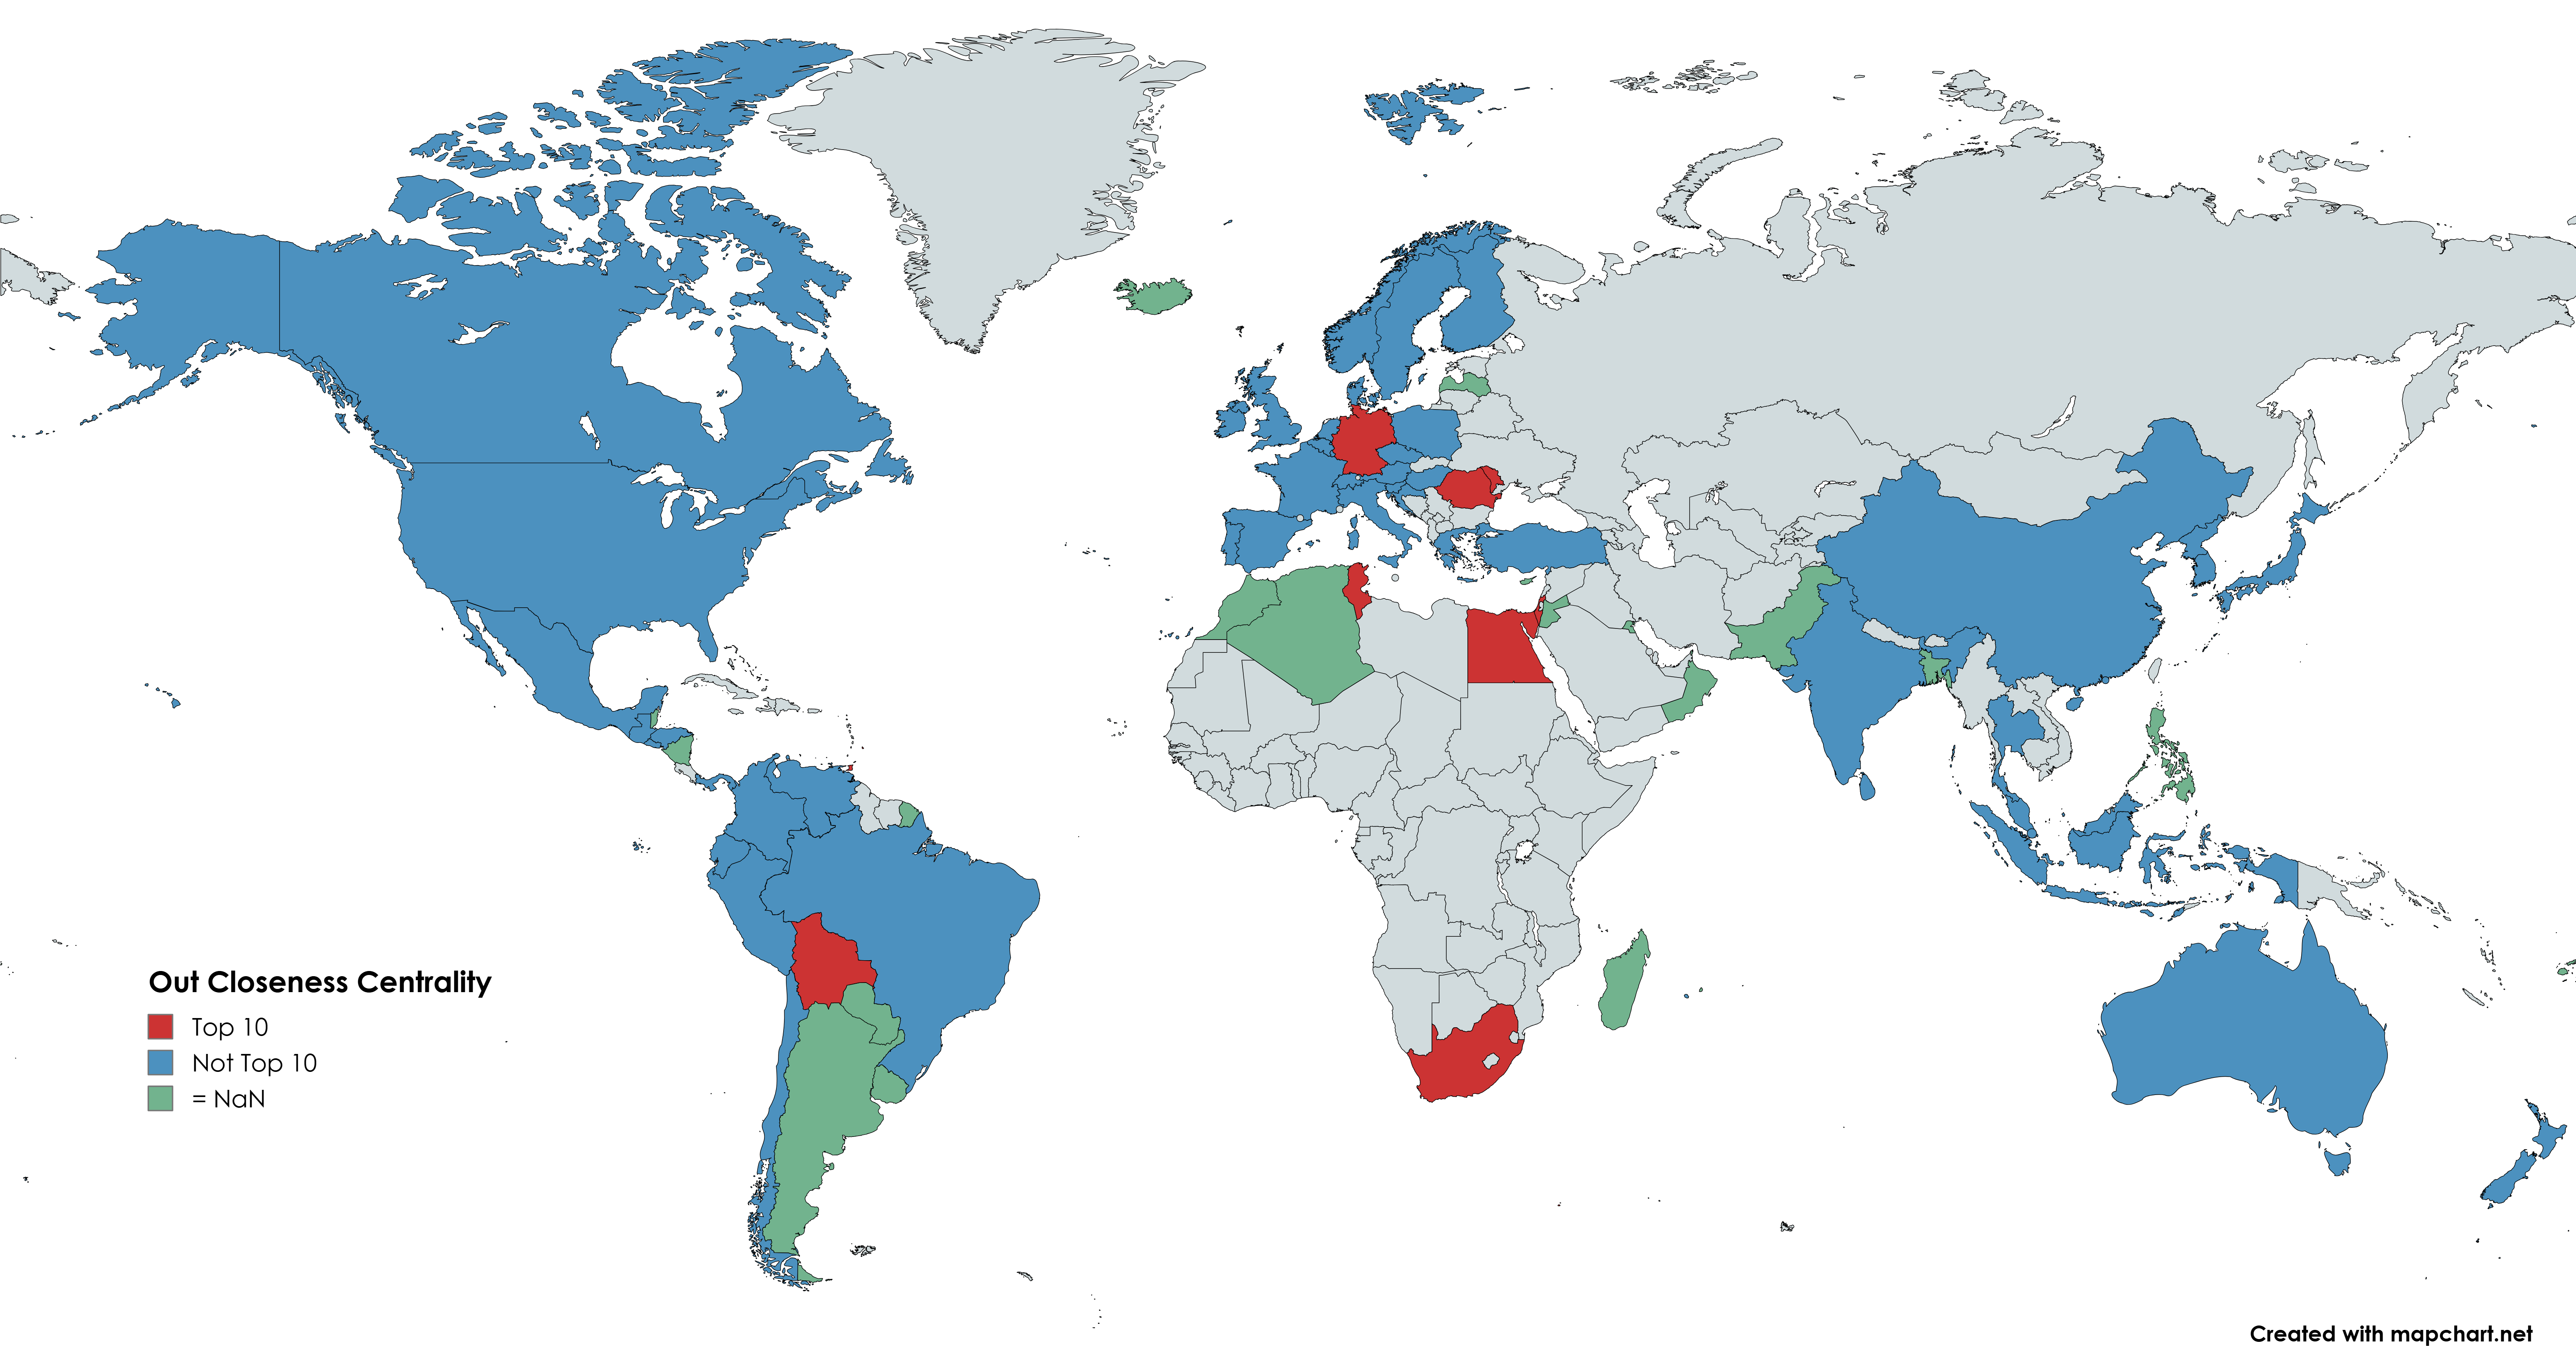
\includegraphics{imagesWorldMaps/Out_Closeness_Centrality.png}

Top 10 Nazioni rispetto all'Out Closeness

    \begin{tcolorbox}[breakable, size=fbox, boxrule=1pt, pad at break*=1mm,colback=cellbackground, colframe=cellborder]
\prompt{In}{incolor}{17}{\boxspacing}
\begin{Verbatim}[commandchars=\\\{\}]
\PY{n+nf}{centr\PYZus{}clo}\PY{p}{(}\PY{n}{g}\PY{p}{,}\PY{+w}{ }\PY{n}{mode}\PY{+w}{ }\PY{o}{=}\PY{+w}{ }\PY{l+s}{\PYZdq{}}\PY{l+s}{out\PYZdq{}}\PY{p}{)}\PY{o}{\PYZdl{}}\PY{n}{centralization}
\end{Verbatim}
\end{tcolorbox}

    NaN

    
    \paragraph{Conclusioni}\label{conclusioni}

\begin{itemize}
\tightlist
\item
  Nella Rete sono presenti nodi con Out Closeness pari a infinito,
  questo è dato dal fatto che esistono nodi che non inviano collegamenti
  (come abbiamo visto nell'Out Degree)
\item
  La maggior parte dei nodi presenta un Out Closeness \textless{} 0.1
\item
  Il valore di centralizzazione non è disponibile dato che esistono
  valori per il quale l'Out Closeness è infinito
\end{itemize}

    \subsection{Betweenness Centrality}\label{betweenness-centrality}

Nel nostro caso potremmo interpretare la Betweenness Centrality come una
misura di quanto uno specifico nodo faccia da tramite per il commercio
fra i paesi

    \begin{tcolorbox}[breakable, size=fbox, boxrule=1pt, pad at break*=1mm,colback=cellbackground, colframe=cellborder]
\prompt{In}{incolor}{18}{\boxspacing}
\begin{Verbatim}[commandchars=\\\{\}]
\PY{n}{betweenness}\PY{+w}{ }\PY{o}{\PYZlt{}\PYZhy{}}\PY{+w}{ }\PY{n+nf}{betweenness}\PY{p}{(}\PY{n}{g}\PY{p}{,}\PY{+w}{ }\PY{n}{directed}\PY{+w}{ }\PY{o}{=}\PY{+w}{ }\PY{k+kc}{TRUE}\PY{p}{)}
\end{Verbatim}
\end{tcolorbox}

    I dati da noi ottenuti per la Betweenness Centrality sono i seguenti:

    \begin{tcolorbox}[breakable, size=fbox, boxrule=1pt, pad at break*=1mm,colback=cellbackground, colframe=cellborder]
\prompt{In}{incolor}{19}{\boxspacing}
\begin{Verbatim}[commandchars=\\\{\}]
\PY{c+c1}{\PYZsh{} Istogramma della Betweenness Centrality}
\PY{n+nf}{hist}\PY{p}{(}\PY{n}{betweenness}\PY{p}{)}
\end{Verbatim}
\end{tcolorbox}

    \begin{center}
    \adjustimage{max size={0.9\linewidth}{0.9\paperheight}}{relazioneProgetto_files/relazioneProgetto_47_0.png}
    \end{center}
    { \hspace*{\fill} \\}
    
    \begin{tcolorbox}[breakable, size=fbox, boxrule=1pt, pad at break*=1mm,colback=cellbackground, colframe=cellborder]
\prompt{In}{incolor}{20}{\boxspacing}
\begin{Verbatim}[commandchars=\\\{\}]
\PY{n+nf}{summary}\PY{p}{(}\PY{n}{betweenness}\PY{p}{)}
\end{Verbatim}
\end{tcolorbox}

    
    \begin{Verbatim}[commandchars=\\\{\}]
   Min. 1st Qu.  Median    Mean 3rd Qu.    Max. 
  0.000   0.000   8.899  90.763  60.417 899.793 
    \end{Verbatim}

    
    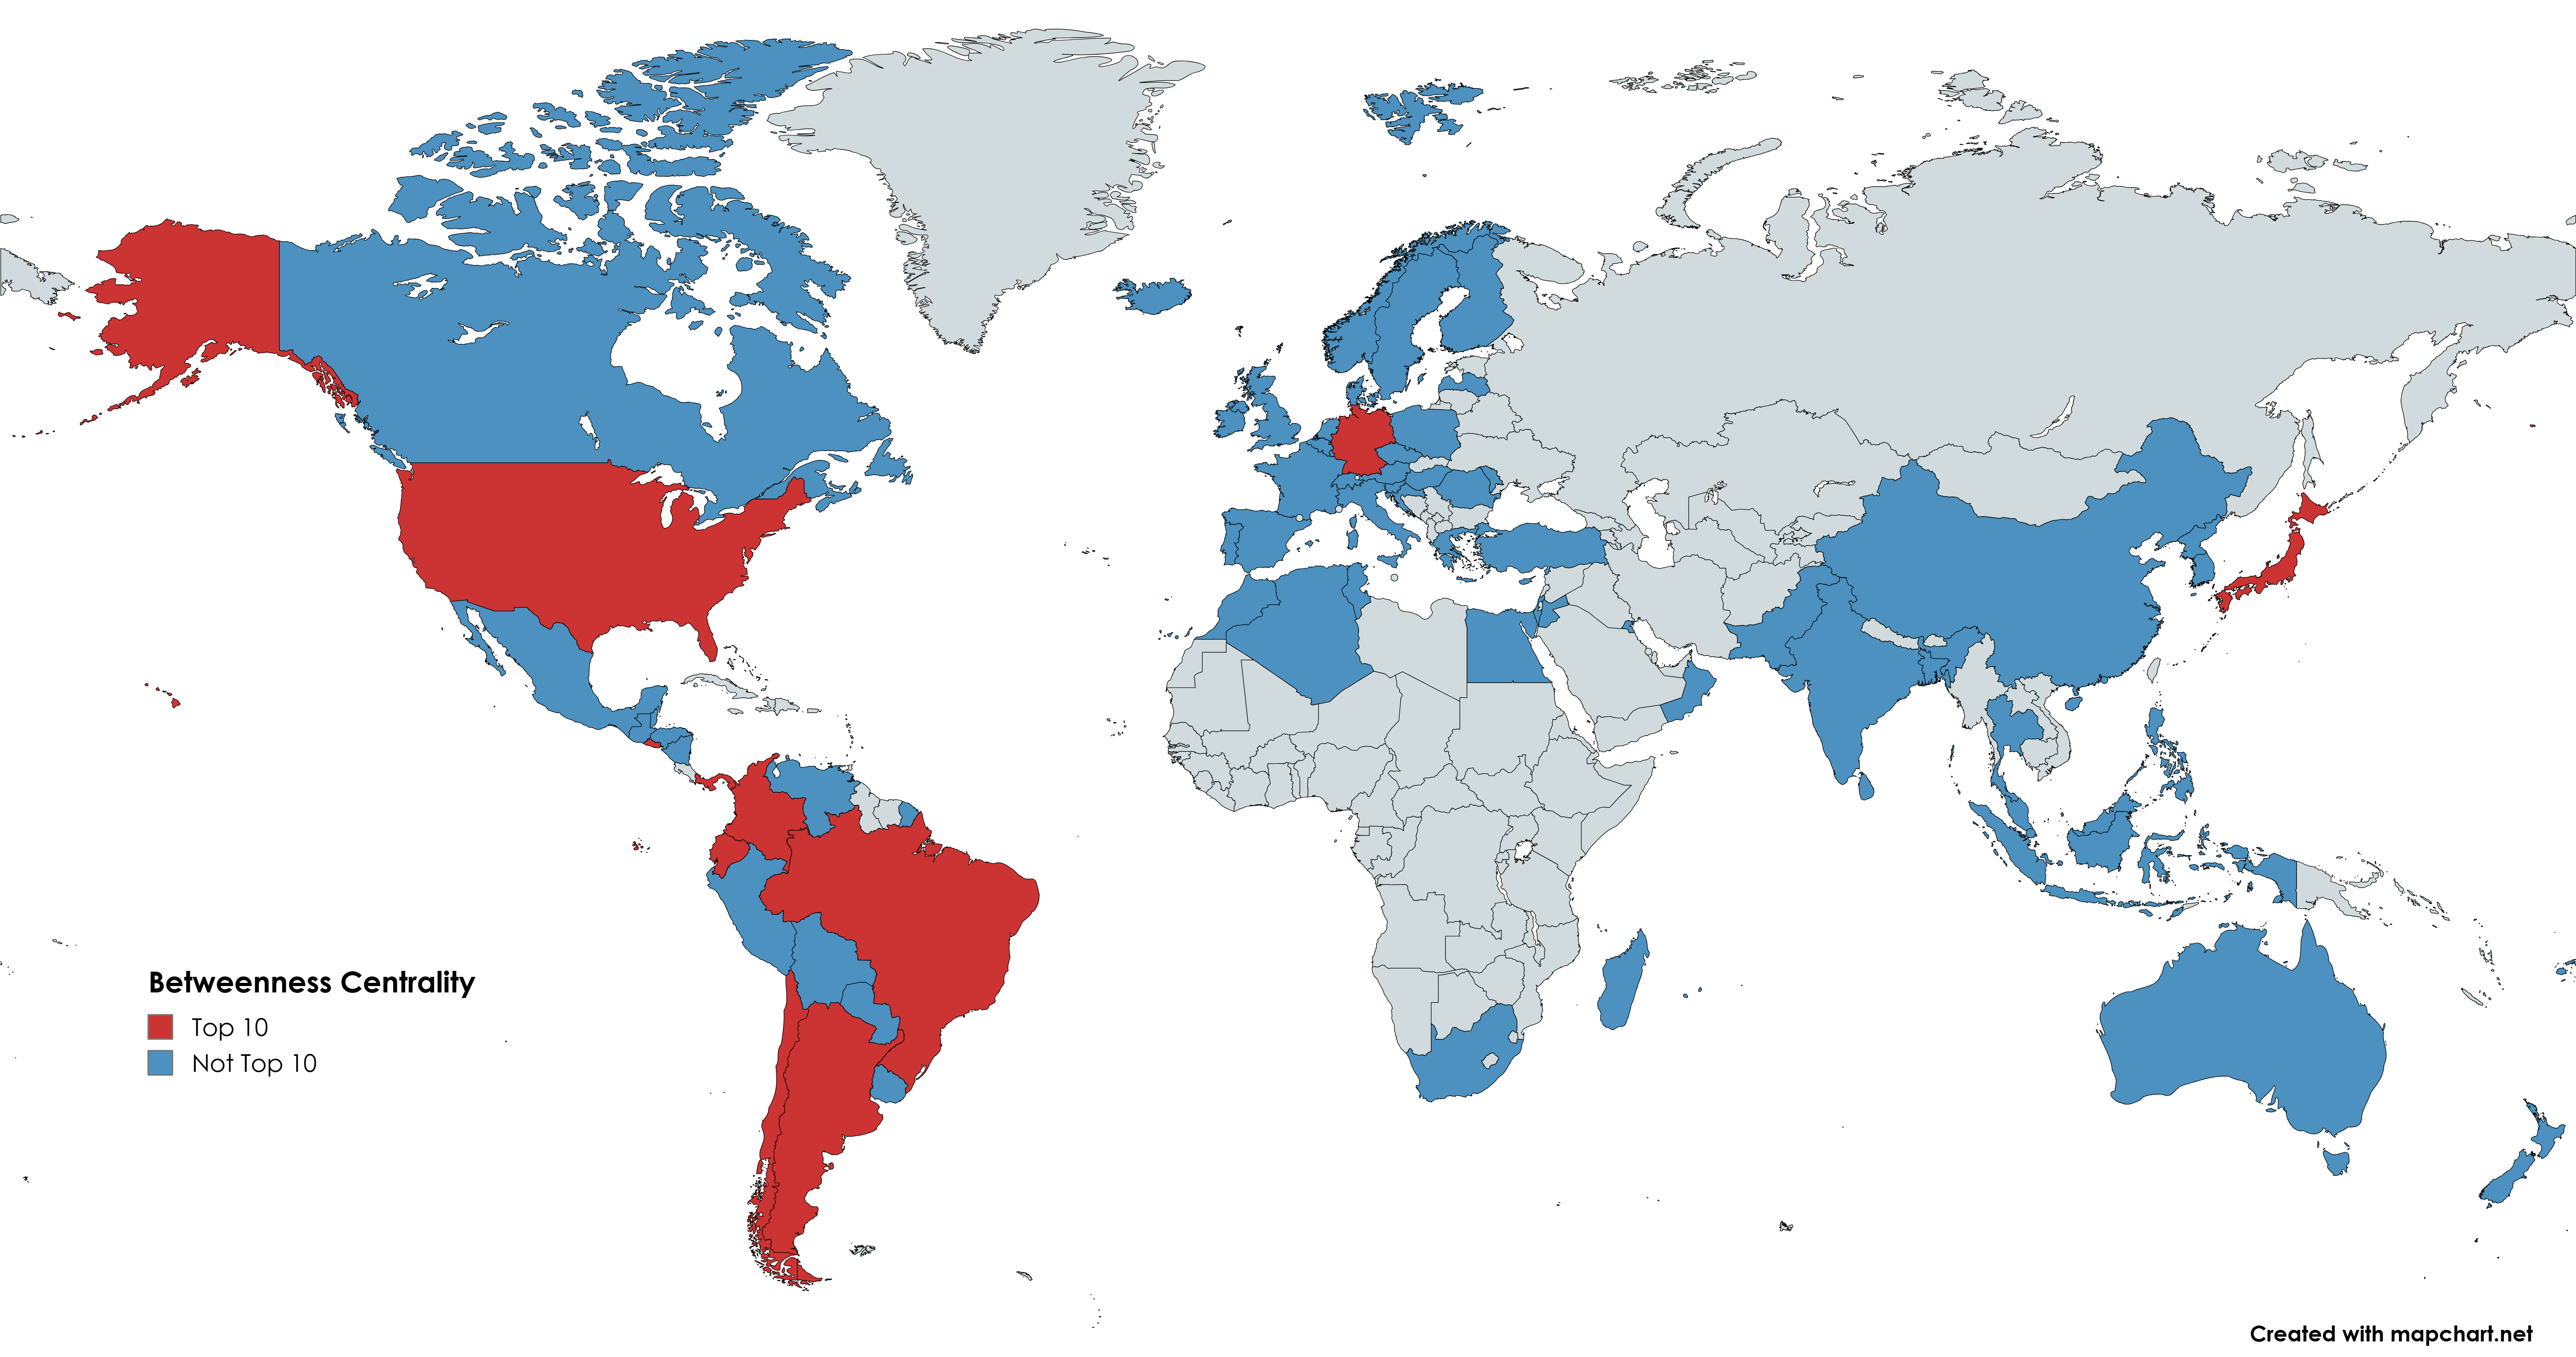
\includegraphics{imagesWorldMaps/Betweenness_Centrality.png}

Top 10 Nazioni rispetto alla Betweenness

    \begin{tcolorbox}[breakable, size=fbox, boxrule=1pt, pad at break*=1mm,colback=cellbackground, colframe=cellborder]
\prompt{In}{incolor}{21}{\boxspacing}
\begin{Verbatim}[commandchars=\\\{\}]
\PY{n+nf}{centr\PYZus{}betw}\PY{p}{(}\PY{n}{g}\PY{p}{,}\PY{+w}{ }\PY{n}{directed}\PY{+w}{ }\PY{o}{=}\PY{+w}{ }\PY{k+kc}{TRUE}\PY{p}{)}\PY{o}{\PYZdl{}}\PY{n}{centralization}
\end{Verbatim}
\end{tcolorbox}

    0.132955452527705

    
    \paragraph{Conclusioni}\label{conclusioni}

\begin{itemize}
\tightlist
\item
  Dall'istogramma si può notare che molti paesi hanno una Betweenness
  bassa
\item
  Se interpretiamo la Betweenness centrality come la capacità di fare da
  ``tramite'' tra due paesi, dato che la transitività (e in particolare
  tau) è molto alta, non sembrerebbe esserci la necessità, infatti il
  valore di centralizzazione è molto vicino allo 0.
\end{itemize}

    \subsection{EigenVector Centrality}\label{eigenvector-centrality}

    \begin{tcolorbox}[breakable, size=fbox, boxrule=1pt, pad at break*=1mm,colback=cellbackground, colframe=cellborder]
\prompt{In}{incolor}{22}{\boxspacing}
\begin{Verbatim}[commandchars=\\\{\}]
\PY{n}{eigen\PYZus{}centrality}\PY{+w}{ }\PY{o}{\PYZlt{}\PYZhy{}}\PY{+w}{ }\PY{n+nf}{eigen\PYZus{}centrality}\PY{p}{(}\PY{n}{g}\PY{p}{)}\PY{o}{\PYZdl{}}\PY{n}{vector}
\end{Verbatim}
\end{tcolorbox}

    I Dati da noi ottenuti per la EigenVector Centrality sono i seguenti:

    \begin{tcolorbox}[breakable, size=fbox, boxrule=1pt, pad at break*=1mm,colback=cellbackground, colframe=cellborder]
\prompt{In}{incolor}{23}{\boxspacing}
\begin{Verbatim}[commandchars=\\\{\}]
\PY{c+c1}{\PYZsh{} Istrogramma dell\PYZsq{}EigenVector Centrality}
\PY{n+nf}{hist}\PY{p}{(}\PY{n}{eigen\PYZus{}centrality}\PY{p}{)}
\end{Verbatim}
\end{tcolorbox}

    \begin{center}
    \adjustimage{max size={0.9\linewidth}{0.9\paperheight}}{relazioneProgetto_files/relazioneProgetto_55_0.png}
    \end{center}
    { \hspace*{\fill} \\}
    
    \begin{tcolorbox}[breakable, size=fbox, boxrule=1pt, pad at break*=1mm,colback=cellbackground, colframe=cellborder]
\prompt{In}{incolor}{24}{\boxspacing}
\begin{Verbatim}[commandchars=\\\{\}]
\PY{n+nf}{summary}\PY{p}{(}\PY{n}{eigen\PYZus{}centrality}\PY{p}{)}
\end{Verbatim}
\end{tcolorbox}

    
    \begin{Verbatim}[commandchars=\\\{\}]
   Min. 1st Qu.  Median    Mean 3rd Qu.    Max. 
0.08979 0.19907 0.28056 0.34384 0.36383 1.00000 
    \end{Verbatim}

    
    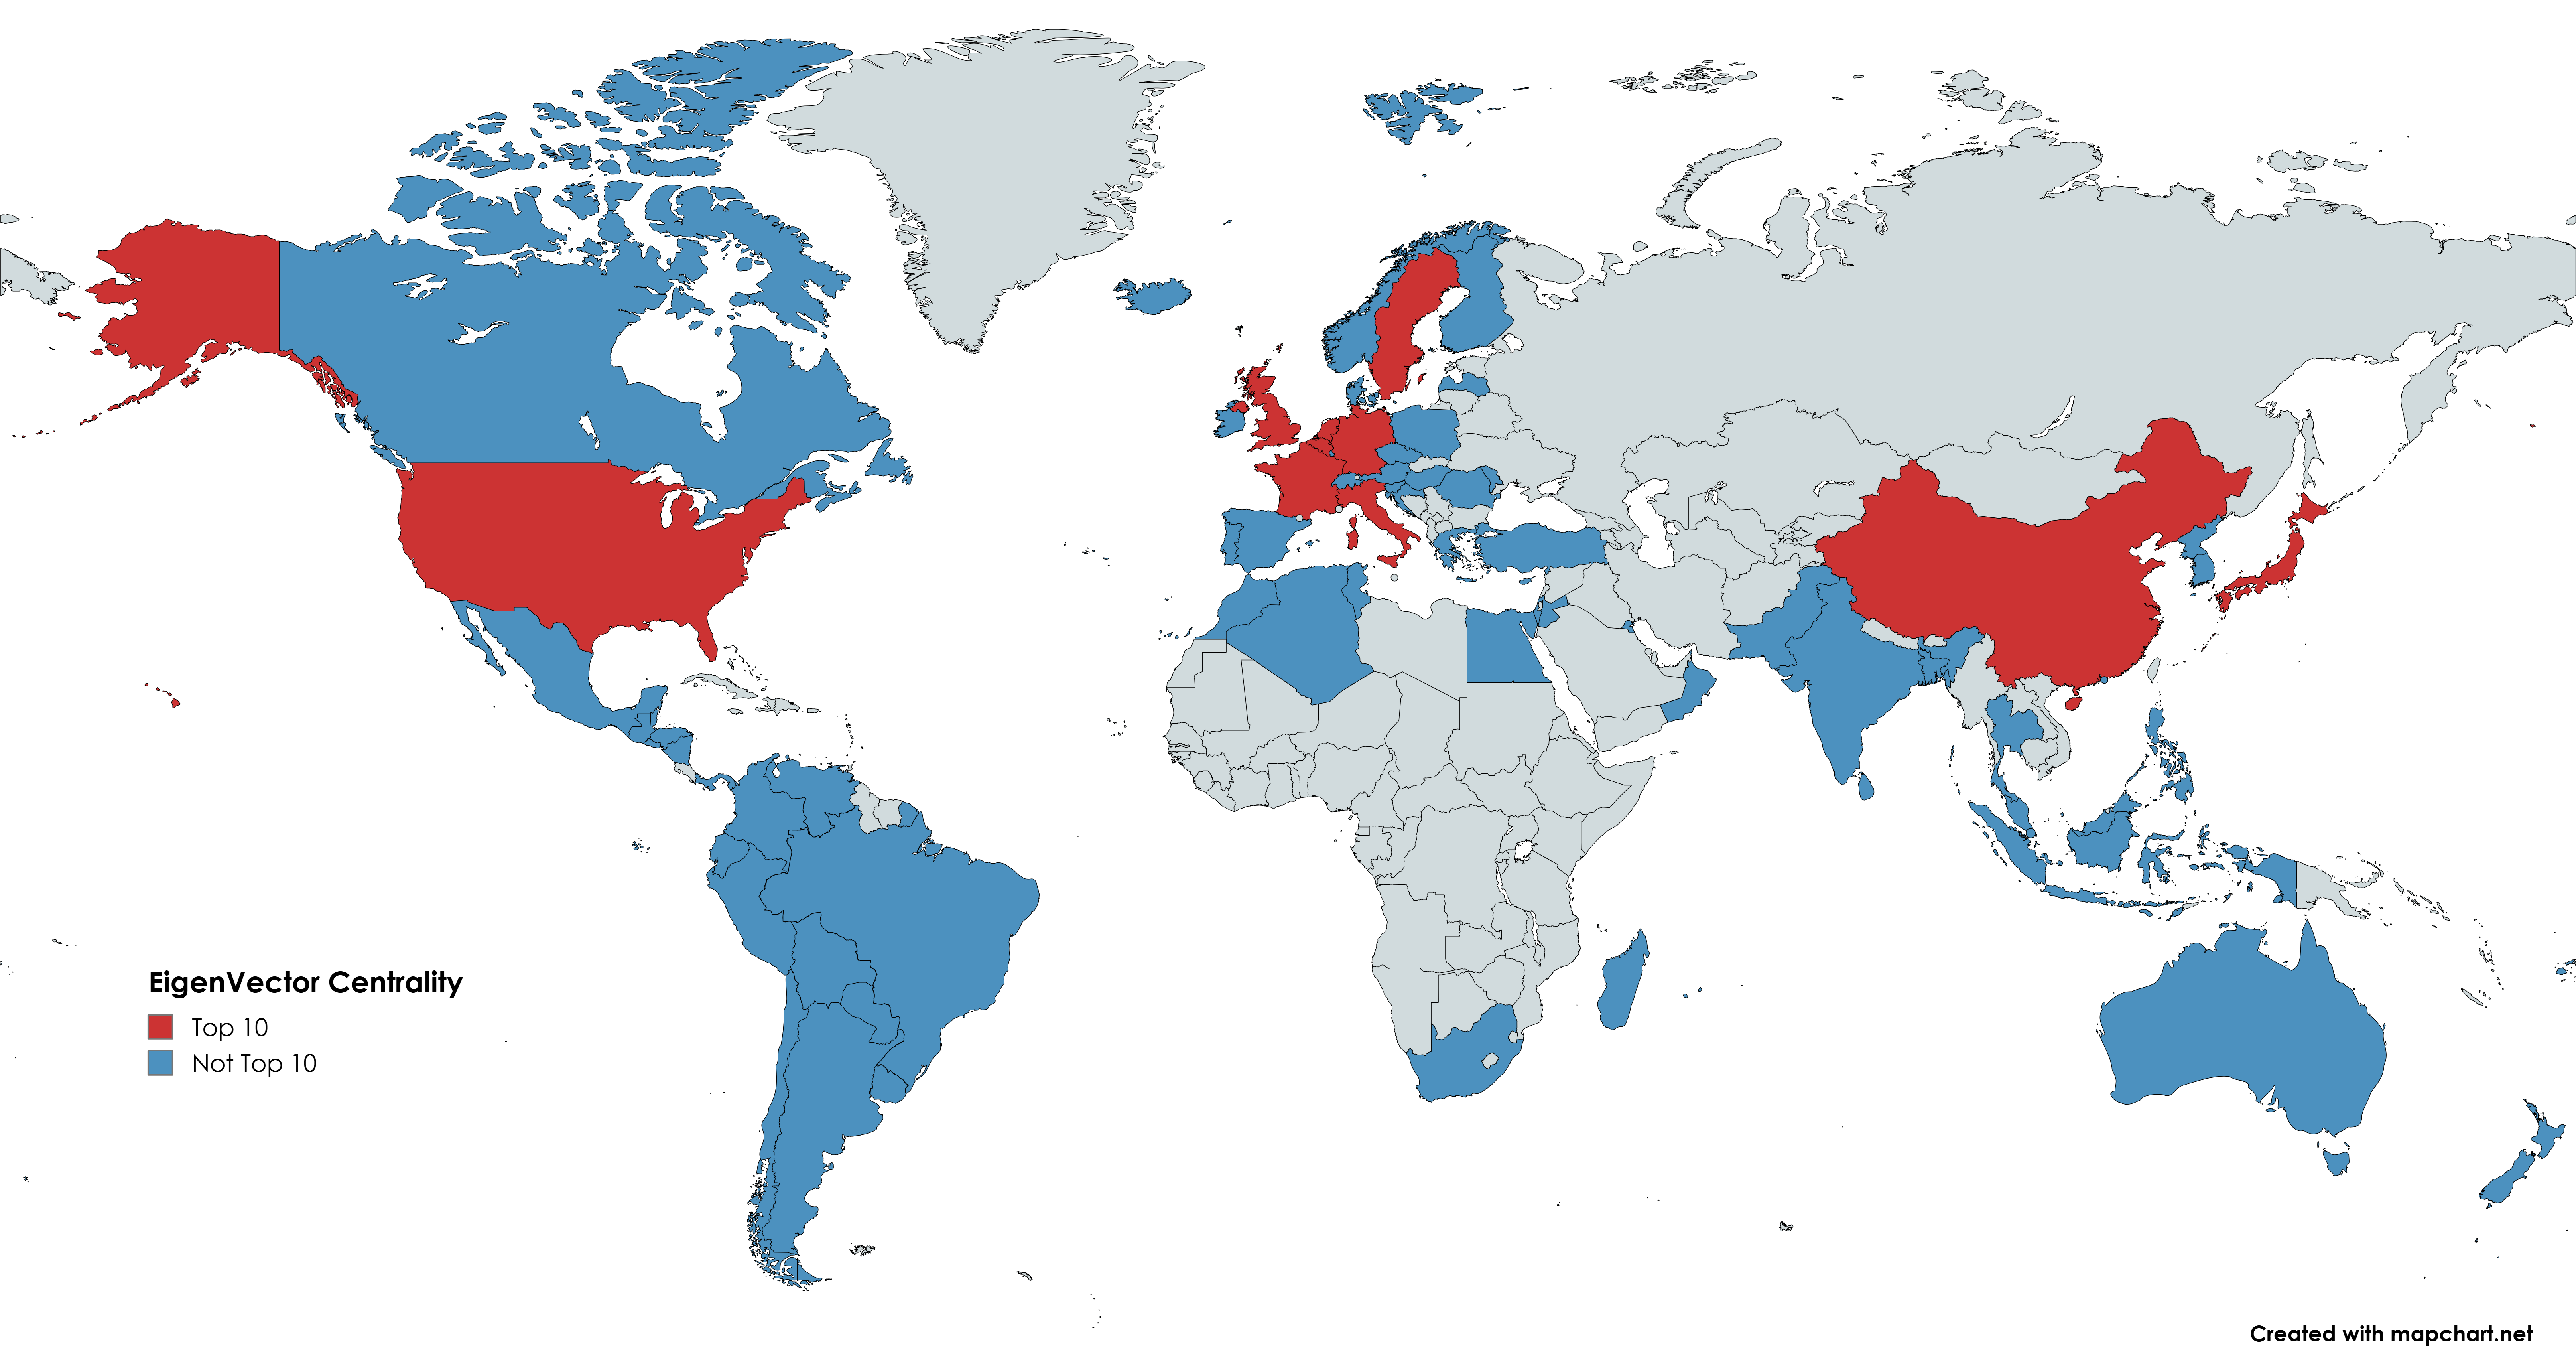
\includegraphics{imagesWorldMaps/EigenVector_Centrality.png}

Top 10 Nazioni rispetto all'EigenVector Value

    \paragraph{Conclusioni}\label{conclusioni}

\begin{itemize}
\tightlist
\item
  Anche in questo caso i Top 10 sono i Paesi più sviluppati, che abbiamo
  menzionato in precedenza (nell'Out Degree)
\end{itemize}

    \section{Modelli}\label{modelli}

    \subsection{Simple Random Graph Model
(SRG)}\label{simple-random-graph-model-srg}

    Breve Introduzione al SRG

Adesso andiamo ad analizzare il SRG model, che rappresenta una base di
partenza per tutti gli altri modelli

    \begin{tcolorbox}[breakable, size=fbox, boxrule=1pt, pad at break*=1mm,colback=cellbackground, colframe=cellborder]
\prompt{In}{incolor}{25}{\boxspacing}
\begin{Verbatim}[commandchars=\\\{\}]
\PY{n+nf}{summary}\PY{p}{(}\PY{n}{model\PYZus{}SRG}\PY{p}{)}
\end{Verbatim}
\end{tcolorbox}

    
    \begin{Verbatim}[commandchars=\\\{\}]
Call:
ergm(formula = net \textasciitilde{} edges, control = control.ergm(seed = 1, 
    checkpoint = "mod0\_step\_\%03d.RData"))

Maximum Likelihood Results:

      Estimate Std. Error MCMC \% z value Pr(>|z|)    
edges -1.67385    0.03449      0  -48.52   <1e-04 ***
---
Signif. codes:  0 '***' 0.001 '**' 0.01 '*' 0.05 '.' 0.1 ' ' 1

     Null Deviance: 8761  on 6320  degrees of freedom
 Residual Deviance: 5513  on 6319  degrees of freedom
 
AIC: 5515  BIC: 5522  (Smaller is better. MC Std. Err. = 0)
    \end{Verbatim}

    
    Simuliamo il SRG model e vediamo quali statistiche riesce a catturare e
quali no, così da avere una base di partenza per i modelli che andremo a
creare

    \begin{tcolorbox}[breakable, size=fbox, boxrule=1pt, pad at break*=1mm,colback=cellbackground, colframe=cellborder]
\prompt{In}{incolor}{26}{\boxspacing}
\begin{Verbatim}[commandchars=\\\{\}]
\PY{n}{extractInformationsFromGraph}\PY{+w}{ }\PY{o}{\PYZlt{}\PYZhy{}}\PY{+w}{ }\PY{n+nf}{function}\PY{p}{(}\PY{n}{xx}\PY{p}{)}\PY{p}{\PYZob{}}
\PY{+w}{	}\PY{n}{ig}\PY{+w}{ }\PY{o}{\PYZlt{}\PYZhy{}}\PY{+w}{ }\PY{n+nf}{asIgraph}\PY{p}{(}\PY{n}{xx}\PY{p}{)}
\PY{+w}{	}\PY{n}{tr}\PY{+w}{ }\PY{o}{\PYZlt{}\PYZhy{}}\PY{+w}{ }\PY{n+nf}{transitivity}\PY{p}{(}\PY{n}{ig}\PY{p}{)}
\PY{+w}{	}\PY{n}{ideg}\PY{+w}{ }\PY{o}{\PYZlt{}\PYZhy{}}\PY{+w}{ }\PY{n+nf}{sd}\PY{p}{(}\PY{n+nf}{degree}\PY{p}{(}\PY{n}{ig}\PY{p}{,}\PY{+w}{ }\PY{n}{mode}\PY{+w}{ }\PY{o}{=}\PY{+w}{ }\PY{l+s}{\PYZdq{}}\PY{l+s}{in\PYZdq{}}\PY{p}{)}\PY{p}{)}
\PY{+w}{	}\PY{n}{odeg}\PY{+w}{ }\PY{o}{\PYZlt{}\PYZhy{}}\PY{+w}{ }\PY{n+nf}{sd}\PY{p}{(}\PY{n+nf}{degree}\PY{p}{(}\PY{n}{ig}\PY{p}{,}\PY{+w}{ }\PY{n}{mode}\PY{+w}{ }\PY{o}{=}\PY{+w}{ }\PY{l+s}{\PYZdq{}}\PY{l+s}{out\PYZdq{}}\PY{p}{)}\PY{p}{)}
\PY{+w}{	}\PY{n}{dens}\PY{+w}{ }\PY{o}{\PYZlt{}\PYZhy{}}\PY{+w}{ }\PY{n+nf}{edge\PYZus{}density}\PY{p}{(}\PY{n}{ig}\PY{p}{)}
\PY{+w}{	}\PY{n+nf}{return}\PY{p}{(}\PY{n+nf}{c}\PY{p}{(}\PY{n}{tr}\PY{p}{,}\PY{+w}{ }\PY{n}{ideg}\PY{p}{,}\PY{+w}{ }\PY{n}{odeg}\PY{p}{,}\PY{+w}{ }\PY{n}{dens}\PY{p}{)}\PY{p}{)}
\PY{p}{\PYZcb{}}

\PY{n}{sim\PYZus{}SRG}\PY{+w}{ }\PY{o}{\PYZlt{}\PYZhy{}}\PY{+w}{ }\PY{n+nf}{suppressMessages}\PY{p}{(}\PY{n+nf}{simulate}\PY{p}{(}\PY{n}{model\PYZus{}SRG}\PY{p}{,}\PY{+w}{ }\PY{n}{nsim}\PY{+w}{ }\PY{o}{=}\PY{+w}{ }\PY{l+m}{100}\PY{p}{,}\PY{+w}{ }\PY{n}{verbose}\PY{+w}{ }\PY{o}{=}\PY{+w}{ }\PY{k+kc}{TRUE}\PY{p}{,}\PY{+w}{ }\PY{n}{seed}\PY{+w}{ }\PY{o}{=}\PY{+w}{ }\PY{l+m}{1}\PY{p}{)}\PY{p}{)}

\PY{n}{null.distr\PYZus{}SRG}\PY{+w}{ }\PY{o}{\PYZlt{}\PYZhy{}}\PY{+w}{ }\PY{n+nf}{matrix}\PY{p}{(}\PY{p}{,}\PY{l+m}{100}\PY{p}{,}\PY{l+m}{4}\PY{p}{)}
\PY{n+nf}{for}\PY{p}{(}\PY{n}{b}\PY{+w}{ }\PY{n}{in}\PY{+w}{ }\PY{l+m}{1}\PY{o}{:}\PY{l+m}{100}\PY{p}{)}\PY{p}{\PYZob{}}
\PY{+w}{	}\PY{n}{null.distr\PYZus{}SRG}\PY{p}{[}\PY{n}{b}\PY{p}{,}\PY{p}{]}\PY{+w}{ }\PY{o}{\PYZlt{}\PYZhy{}}\PY{+w}{ }\PY{n+nf}{extractInformationsFromGraph}\PY{p}{(}\PY{n}{sim\PYZus{}SRG}\PY{p}{[[}\PY{n}{b}\PY{p}{]]}\PY{p}{)}
\PY{p}{\PYZcb{}}

\PY{n+nf}{par}\PY{p}{(}\PY{n}{mfrow}\PY{+w}{ }\PY{o}{=}\PY{+w}{ }\PY{n+nf}{c}\PY{p}{(}\PY{l+m}{4}\PY{p}{,}\PY{l+m}{1}\PY{p}{)}\PY{p}{)}
\PY{n+nf}{hist}\PY{p}{(}\PY{n+nf}{unlist}\PY{p}{(}\PY{n}{null.distr\PYZus{}SRG}\PY{p}{[}\PY{p}{,}\PY{l+m}{2}\PY{p}{]}\PY{p}{)}\PY{p}{,}\PY{+w}{ }\PY{n}{xlab}\PY{+w}{ }\PY{o}{=}\PY{+w}{ }\PY{l+s}{\PYZdq{}}\PY{l+s}{in\PYZhy{}degree\PYZdq{}}\PY{p}{,}\PY{+w}{ }\PY{n}{xlim}\PY{+w}{ }\PY{o}{=}\PY{+w}{ }\PY{n+nf}{c}\PY{p}{(}\PY{l+m}{2}\PY{p}{,}\PY{l+m}{5}\PY{p}{)}\PY{p}{,}\PY{+w}{ }\PY{n}{main}\PY{+w}{ }\PY{o}{=}\PY{+w}{ }\PY{l+s}{\PYZdq{}}\PY{l+s}{In Degree Distribution on SRG\PYZdq{}}\PY{p}{)}\PY{p}{;}\PY{+w}{ }\PY{n+nf}{abline}\PY{p}{(}\PY{n}{v}\PY{+w}{ }\PY{o}{=}\PY{+w}{ }\PY{n+nf}{sd}\PY{p}{(}\PY{n+nf}{degree}\PY{p}{(}\PY{n}{g}\PY{p}{,}\PY{+w}{ }\PY{n}{mode}\PY{+w}{ }\PY{o}{=}\PY{+w}{ }\PY{l+s}{\PYZdq{}}\PY{l+s}{in\PYZdq{}}\PY{p}{)}\PY{p}{)}\PY{p}{,}\PY{+w}{ }\PY{n}{col}\PY{+w}{ }\PY{o}{=}\PY{+w}{ }\PY{l+s}{\PYZdq{}}\PY{l+s}{red\PYZdq{}}\PY{p}{)}
\PY{n+nf}{hist}\PY{p}{(}\PY{n+nf}{unlist}\PY{p}{(}\PY{n}{null.distr\PYZus{}SRG}\PY{p}{[}\PY{p}{,}\PY{l+m}{3}\PY{p}{]}\PY{p}{)}\PY{p}{,}\PY{+w}{ }\PY{n}{xlab}\PY{+w}{ }\PY{o}{=}\PY{+w}{ }\PY{l+s}{\PYZdq{}}\PY{l+s}{out\PYZhy{}degree\PYZdq{}}\PY{p}{,}\PY{+w}{ }\PY{n}{xlim}\PY{o}{=}\PY{n+nf}{c}\PY{p}{(}\PY{l+m}{0}\PY{p}{,}\PY{+w}{ }\PY{l+m}{22}\PY{p}{)}\PY{p}{,}\PY{+w}{ }\PY{n}{main}\PY{+w}{ }\PY{o}{=}\PY{+w}{ }\PY{l+s}{\PYZdq{}}\PY{l+s}{Out Degree Distribution on SRG\PYZdq{}}\PY{p}{)}\PY{p}{;}\PY{+w}{ }\PY{n+nf}{abline}\PY{p}{(}\PY{n}{v}\PY{+w}{ }\PY{o}{=}\PY{+w}{ }\PY{n+nf}{sd}\PY{p}{(}\PY{n+nf}{degree}\PY{p}{(}\PY{n}{g}\PY{p}{,}\PY{+w}{ }\PY{n}{mode}\PY{+w}{ }\PY{o}{=}\PY{+w}{ }\PY{l+s}{\PYZdq{}}\PY{l+s}{out\PYZdq{}}\PY{p}{)}\PY{p}{)}\PY{p}{,}\PY{+w}{ }\PY{n}{col}\PY{+w}{ }\PY{o}{=}\PY{+w}{ }\PY{l+s}{\PYZdq{}}\PY{l+s}{red\PYZdq{}}\PY{p}{)}
\PY{n+nf}{hist}\PY{p}{(}\PY{n+nf}{unlist}\PY{p}{(}\PY{n}{null.distr\PYZus{}SRG}\PY{p}{[}\PY{p}{,}\PY{l+m}{1}\PY{p}{]}\PY{p}{)}\PY{p}{,}\PY{+w}{ }\PY{n}{xlab}\PY{+w}{ }\PY{o}{=}\PY{+w}{ }\PY{l+s}{\PYZdq{}}\PY{l+s}{transitivity\PYZdq{}}\PY{p}{,}\PY{+w}{ }\PY{n}{xlim}\PY{o}{=}\PY{n+nf}{c}\PY{p}{(}\PY{l+m}{0.2}\PY{p}{,}\PY{+w}{ }\PY{l+m}{0.5}\PY{p}{)}\PY{p}{,}\PY{+w}{ }\PY{n}{main}\PY{+w}{ }\PY{o}{=}\PY{+w}{ }\PY{l+s}{\PYZdq{}}\PY{l+s}{Transitivity Distribution on SRG\PYZdq{}}\PY{p}{)}\PY{p}{;}\PY{+w}{ }\PY{n+nf}{abline}\PY{p}{(}\PY{n}{v}\PY{+w}{ }\PY{o}{=}\PY{+w}{ }\PY{n+nf}{transitivity}\PY{p}{(}\PY{n}{g}\PY{p}{)}\PY{p}{,}\PY{+w}{ }\PY{n}{col}\PY{+w}{ }\PY{o}{=}\PY{+w}{ }\PY{l+s}{\PYZdq{}}\PY{l+s}{red\PYZdq{}}\PY{p}{)}
\PY{n+nf}{hist}\PY{p}{(}\PY{n+nf}{unlist}\PY{p}{(}\PY{n}{null.distr\PYZus{}SRG}\PY{p}{[}\PY{p}{,}\PY{l+m}{4}\PY{p}{]}\PY{p}{)}\PY{p}{,}\PY{+w}{ }\PY{n}{xlab}\PY{+w}{ }\PY{o}{=}\PY{+w}{ }\PY{l+s}{\PYZdq{}}\PY{l+s}{density\PYZdq{}}\PY{p}{,}\PY{+w}{ }\PY{n}{main}\PY{+w}{ }\PY{o}{=}\PY{+w}{ }\PY{l+s}{\PYZdq{}}\PY{l+s}{Density Distribution on SRG\PYZdq{}}\PY{p}{)}\PY{p}{;}\PY{+w}{ }\PY{n+nf}{abline}\PY{p}{(}\PY{n}{v}\PY{+w}{ }\PY{o}{=}\PY{+w}{ }\PY{n+nf}{edge\PYZus{}density}\PY{p}{(}\PY{n}{g}\PY{p}{)}\PY{p}{,}\PY{+w}{ }\PY{n}{col}\PY{+w}{ }\PY{o}{=}\PY{+w}{ }\PY{l+s}{\PYZdq{}}\PY{l+s}{red\PYZdq{}}\PY{p}{)}
\end{Verbatim}
\end{tcolorbox}

    \begin{center}
    \adjustimage{max size={0.9\linewidth}{0.9\paperheight}}{relazioneProgetto_files/relazioneProgetto_64_0.png}
    \end{center}
    { \hspace*{\fill} \\}
    
    Il nostro attuale modello è in grado di catturare la densità (come
potevamo aspettarci) e la In-Degree.

    \subsection{Exponential Random Graph Models
(ERGMs)}\label{exponential-random-graph-models-ergms}

    \subsubsection{Non-Homogeneus Simple Random Graph Model
(NH-SRG)}\label{non-homogeneus-simple-random-graph-model-nh-srg}

    Breve Introduzione al NH-SRG e differenze con SRG

Adesso andiamo ad analizzare i risultati ottenuti dal calcolo del NH-SRG
model

    \begin{tcolorbox}[breakable, size=fbox, boxrule=1pt, pad at break*=1mm,colback=cellbackground, colframe=cellborder]
\prompt{In}{incolor}{ }{\boxspacing}
\begin{Verbatim}[commandchars=\\\{\}]
\PY{n+nf}{summary}\PY{p}{(}\PY{n}{model\PYZus{}NHSRG}\PY{p}{)}
\end{Verbatim}
\end{tcolorbox}

    Dato che il summary del NH-SRG richiedeva molto spazio, abbiamo deciso
di inserire degli screenshot.

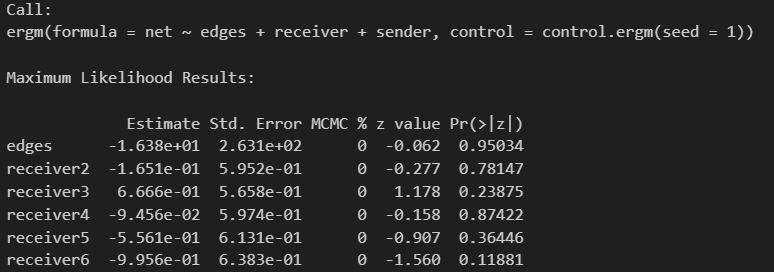
\includegraphics{images/model_NHSRG_p1.png}
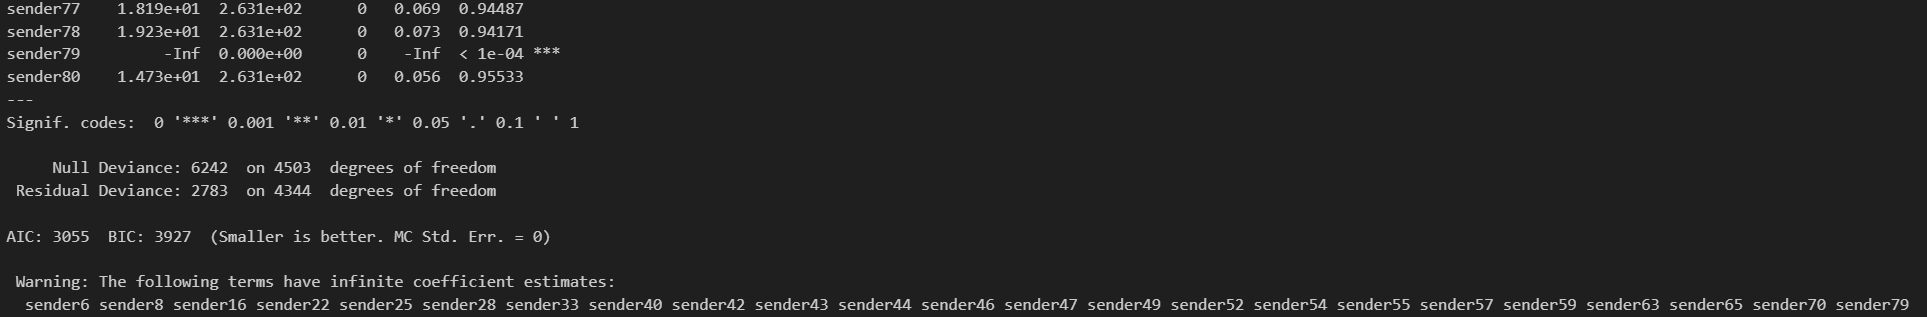
\includegraphics{images/model_NHSRG_p2.png}

    Da come possiamo notare alcuni Sender Effect hanno valore Infinito,
dunque siamo costretti a togliere dal modello il Sender Effect.

    \begin{tcolorbox}[breakable, size=fbox, boxrule=1pt, pad at break*=1mm,colback=cellbackground, colframe=cellborder]
\prompt{In}{incolor}{28}{\boxspacing}
\begin{Verbatim}[commandchars=\\\{\}]
\PY{n+nf}{summary}\PY{p}{(}\PY{n}{model\PYZus{}NHSRG\PYZus{}onlyReceiver}\PY{p}{)}
\end{Verbatim}
\end{tcolorbox}

    
    \begin{Verbatim}[commandchars=\\\{\}]
Call:
ergm(formula = net \textasciitilde{} edges + receiver, control = control.ergm(seed = 1, 
    checkpoint = "mod1\_receiver\_step\_\%03d.RData"))

Maximum Likelihood Results:

             Estimate Std. Error MCMC \% z value Pr(>|z|)    
edges      -1.535e+00  2.946e-01      0  -5.211   <1e-04 ***
receiver2  -8.938e-02  4.230e-01      0  -0.211   0.8326    
receiver3   3.148e-01  3.984e-01      0   0.790   0.4295    
receiver4  -8.938e-02  4.230e-01      0  -0.211   0.8326    
receiver5  -2.863e-01  4.387e-01      0  -0.653   0.5140    
receiver6  -5.159e-01  4.607e-01      0  -1.120   0.2627    
receiver7  -8.938e-02  4.230e-01      0  -0.211   0.8326    
receiver8  -2.863e-01  4.387e-01      0  -0.653   0.5140    
receiver9  -1.845e-01  4.302e-01      0  -0.429   0.6681    
receiver10 -8.938e-02  4.230e-01      0  -0.211   0.8326    
receiver11 -5.159e-01  4.607e-01      0  -1.120   0.2627    
receiver12  2.414e-01  4.022e-01      0   0.600   0.5484    
receiver13 -6.479e-01  4.753e-01      0  -1.363   0.1728    
receiver14 -3.282e-14  4.167e-01      0   0.000   1.0000    
receiver15 -8.938e-02  4.230e-01      0  -0.211   0.8326    
receiver16 -8.938e-02  4.230e-01      0  -0.211   0.8326    
receiver17 -3.962e-01  4.487e-01      0  -0.883   0.3772    
receiver18  8.450e-02  4.112e-01      0   0.205   0.8372    
receiver19 -3.216e-14  4.167e-01      0   0.000   1.0000    
receiver20  8.450e-02  4.112e-01      0   0.205   0.8372    
receiver21 -8.938e-02  4.230e-01      0  -0.211   0.8326    
receiver22 -1.845e-01  4.302e-01      0  -0.429   0.6681    
receiver23  8.450e-02  4.112e-01      0   0.205   0.8372    
receiver24 -3.962e-01  4.487e-01      0  -0.883   0.3772    
receiver25 -1.396e+00  5.917e-01      0  -2.359   0.0183 *  
receiver26  3.148e-01  3.984e-01      0   0.790   0.4295    
receiver27 -8.938e-02  4.230e-01      0  -0.211   0.8326    
receiver28 -1.159e+00  5.480e-01      0  -2.116   0.0344 *  
receiver29 -8.938e-02  4.230e-01      0  -0.211   0.8326    
receiver30 -3.110e-14  4.167e-01      0   0.000   1.0000    
receiver31 -6.479e-01  4.753e-01      0  -1.363   0.1728    
receiver32  8.450e-02  4.112e-01      0   0.205   0.8372    
receiver33 -2.863e-01  4.387e-01      0  -0.653   0.5140    
receiver34 -3.134e-14  4.167e-01      0   0.000   1.0000    
receiver35 -2.971e-14  4.167e-01      0   0.000   1.0000    
receiver36 -3.962e-01  4.487e-01      0  -0.883   0.3772    
receiver37  8.450e-02  4.112e-01      0   0.205   0.8372    
receiver38 -8.938e-02  4.230e-01      0  -0.211   0.8326    
receiver39 -3.128e-14  4.167e-01      0   0.000   1.0000    
receiver40  2.414e-01  4.022e-01      0   0.600   0.5484    
receiver41 -3.962e-01  4.487e-01      0  -0.883   0.3772    
receiver42 -3.962e-01  4.487e-01      0  -0.883   0.3772    
receiver43 -3.962e-01  4.487e-01      0  -0.883   0.3772    
receiver44 -3.090e-14  4.167e-01      0   0.000   1.0000    
receiver45  8.450e-02  4.112e-01      0   0.205   0.8372    
receiver46 -1.159e+00  5.480e-01      0  -2.116   0.0344 *  
receiver47  8.450e-02  4.112e-01      0   0.205   0.8372    
receiver48 -7.954e-01  4.935e-01      0  -1.612   0.1070    
receiver49  8.450e-02  4.112e-01      0   0.205   0.8372    
receiver50 -2.855e-14  4.167e-01      0   0.000   1.0000    
receiver51  1.648e-01  4.064e-01      0   0.405   0.6852    
receiver52 -1.845e-01  4.302e-01      0  -0.429   0.6681    
receiver53 -8.938e-02  4.230e-01      0  -0.211   0.8326    
receiver54 -5.159e-01  4.607e-01      0  -1.120   0.2627    
receiver55 -3.962e-01  4.487e-01      0  -0.883   0.3772    
receiver56 -2.863e-01  4.387e-01      0  -0.653   0.5140    
receiver57 -3.962e-01  4.487e-01      0  -0.883   0.3772    
receiver58  8.450e-02  4.112e-01      0   0.205   0.8372    
receiver59 -3.236e-14  4.167e-01      0   0.000   1.0000    
receiver60  8.450e-02  4.112e-01      0   0.205   0.8372    
receiver61 -2.863e-01  4.387e-01      0  -0.653   0.5140    
receiver62 -1.159e+00  5.480e-01      0  -2.116   0.0344 *  
receiver63 -9.634e-01  5.169e-01      0  -1.864   0.0623 .  
receiver64  1.648e-01  4.064e-01      0   0.405   0.6852    
receiver65 -2.863e-01  4.387e-01      0  -0.653   0.5140    
receiver66  1.648e-01  4.064e-01      0   0.405   0.6852    
receiver67 -3.962e-01  4.487e-01      0  -0.883   0.3772    
receiver68  3.148e-01  3.984e-01      0   0.790   0.4295    
receiver69 -3.097e-14  4.167e-01      0   0.000   1.0000    
receiver70  2.414e-01  4.022e-01      0   0.600   0.5484    
receiver71  1.648e-01  4.064e-01      0   0.405   0.6852    
receiver72 -3.962e-01  4.487e-01      0  -0.883   0.3772    
receiver73 -3.962e-01  4.487e-01      0  -0.883   0.3772    
receiver74 -2.863e-01  4.387e-01      0  -0.653   0.5140    
receiver75 -3.476e-14  4.167e-01      0   0.000   1.0000    
receiver76 -3.066e-14  4.167e-01      0   0.000   1.0000    
receiver77  1.648e-01  4.064e-01      0   0.405   0.6852    
receiver78 -3.344e-14  4.167e-01      0   0.000   1.0000    
receiver79 -2.863e-01  4.387e-01      0  -0.653   0.5140    
receiver80  8.450e-02  4.112e-01      0   0.205   0.8372    
---
Signif. codes:  0 '***' 0.001 '**' 0.01 '*' 0.05 '.' 0.1 ' ' 1

     Null Deviance: 8761  on 6320  degrees of freedom
 Residual Deviance: 5432  on 6240  degrees of freedom
 
AIC: 5592  BIC: 6132  (Smaller is better. MC Std. Err. = 0)
    \end{Verbatim}

    
    Da come si può notare i Receiver Effect hanno dei livelli di
significatività molto bassi, quindi valutiamo la rimozione di essi.

    \begin{tcolorbox}[breakable, size=fbox, boxrule=1pt, pad at break*=1mm,colback=cellbackground, colframe=cellborder]
\prompt{In}{incolor}{29}{\boxspacing}
\begin{Verbatim}[commandchars=\\\{\}]
\PY{n}{table}\PY{+w}{ }\PY{o}{\PYZlt{}\PYZhy{}}\PY{+w}{ }\PY{n+nf}{data.frame}\PY{p}{(}
\PY{+w}{    }\PY{n}{Modelli}\PY{+w}{ }\PY{o}{=}\PY{+w}{ }\PY{n+nf}{c}\PY{p}{(}\PY{l+s}{\PYZdq{}}\PY{l+s}{model\PYZus{}SRG\PYZdq{}}\PY{p}{,}\PY{+w}{ }\PY{l+s}{\PYZdq{}}\PY{l+s}{model\PYZus{}NHSRG\PYZus{}onlyReceiver\PYZdq{}}\PY{p}{)}\PY{p}{,}
\PY{+w}{    }\PY{n}{BIC}\PY{+w}{ }\PY{o}{=}\PY{+w}{ }\PY{n+nf}{BIC}\PY{p}{(}\PY{n}{model\PYZus{}SRG}\PY{p}{,}\PY{+w}{ }\PY{n}{model\PYZus{}NHSRG\PYZus{}onlyReceiver}\PY{p}{)}
\PY{p}{)}
\PY{n+nf}{createImageFromTable}\PY{p}{(}\PY{n}{table}\PY{p}{,}\PY{+w}{ }\PY{l+s}{\PYZdq{}}\PY{l+s}{images/SRG\PYZus{}vs\PYZus{}NHSRG\PYZus{}BIC.png\PYZdq{}}\PY{p}{,}\PY{+w}{ }\PY{l+m}{900}\PY{p}{,}\PY{+w}{ }\PY{l+m}{220}\PY{p}{,}\PY{+w}{ }\PY{l+m}{230}\PY{p}{)}
\end{Verbatim}
\end{tcolorbox}

    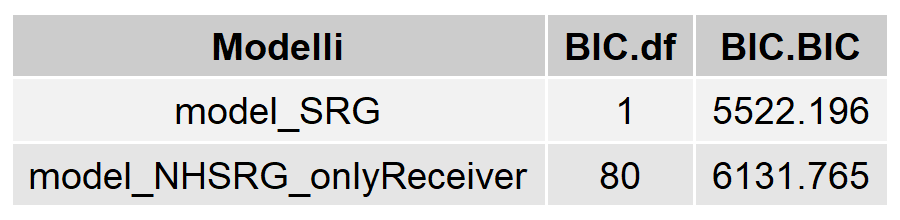
\includegraphics{images/SRG_vs_NHSRG_BIC.png}

    Confrontando quindi questo modello con il modello SRG concludiamo che
togliere il termine Receiver Effect è una buona scelta.

    \subsubsection{P1 Model}\label{p1-model}

    Adesso andiamo ad analizzare i risultati ottenuti per il nostro P1 Model

    \begin{tcolorbox}[breakable, size=fbox, boxrule=1pt, pad at break*=1mm,colback=cellbackground, colframe=cellborder]
\prompt{In}{incolor}{30}{\boxspacing}
\begin{Verbatim}[commandchars=\\\{\}]
\PY{n+nf}{summary}\PY{p}{(}\PY{n}{model\PYZus{}P1\PYZus{}onlyMutual}\PY{p}{)}
\end{Verbatim}
\end{tcolorbox}

    
    \begin{Verbatim}[commandchars=\\\{\}]
Call:
ergm(formula = net \textasciitilde{} edges + mutual, control = control.ergm(seed = 1))

Monte Carlo Maximum Likelihood Results:

       Estimate Std. Error MCMC \% z value Pr(>|z|)    
edges  -1.80765    0.04673      0 -38.684   <1e-04 ***
mutual  0.69042    0.12252      0   5.635   <1e-04 ***
---
Signif. codes:  0 '***' 0.001 '**' 0.01 '*' 0.05 '.' 0.1 ' ' 1

     Null Deviance: 8761  on 6320  degrees of freedom
 Residual Deviance: 5481  on 6318  degrees of freedom
 
AIC: 5485  BIC: 5499  (Smaller is better. MC Std. Err. = 1.073)
    \end{Verbatim}

    
    \subsubsection{Attributi Nodali}\label{attributi-nodali}

    Adesso introduciamo gli effetti principali e di omofilia rispetto agli
Attributi Nodali

    \begin{tcolorbox}[breakable, size=fbox, boxrule=1pt, pad at break*=1mm,colback=cellbackground, colframe=cellborder]
\prompt{In}{incolor}{31}{\boxspacing}
\begin{Verbatim}[commandchars=\\\{\}]
\PY{n+nf}{summary}\PY{p}{(}\PY{n}{model\PYZus{}P1\PYZus{}onlyMutual\PYZus{}NodeAttr}\PY{p}{)}
\end{Verbatim}
\end{tcolorbox}

    
    \begin{Verbatim}[commandchars=\\\{\}]
Call:
ergm(formula = net \textasciitilde{} edges + mutual + nodecov("gdp") + nodefactor("continent") + 
    nodefactor("partition") + absdiff("gdp") + nodematch("continent") + 
    nodematch("partition"), control = control.ergm(seed = 1))

Monte Carlo Maximum Likelihood Results:

                         Estimate Std. Error MCMC \% z value Pr(>|z|)    
edges                   3.074e+00  3.389e-01      0   9.069  < 1e-04 ***
mutual                 -1.912e+00  1.795e-01      0 -10.655  < 1e-04 ***
nodecov.gdp             1.251e-05  4.386e-06      0   2.852 0.004342 ** 
nodefactor.continent.2 -2.665e-02  1.265e-01      0  -0.211 0.833080    
nodefactor.continent.3 -6.301e-01  1.314e-01      0  -4.795  < 1e-04 ***
nodefactor.continent.4  9.280e-01  1.654e-01      0   5.609  < 1e-04 ***
nodefactor.continent.5  7.066e-01  2.123e-01      0   3.328 0.000876 ***
nodefactor.continent.6 -2.808e-02  1.304e-01      0  -0.215 0.829440    
nodefactor.partition.2 -2.834e+00  1.500e-01      0 -18.890  < 1e-04 ***
nodefactor.partition.3 -4.086e+00  1.946e-01      0 -20.993  < 1e-04 ***
absdiff.gdp            -2.512e-05  5.522e-06      0  -4.550  < 1e-04 ***
nodematch.continent     2.257e+00  1.266e-01      0  17.834  < 1e-04 ***
nodematch.partition    -1.908e-01  1.333e-01      0  -1.431 0.152417    
---
Signif. codes:  0 '***' 0.001 '**' 0.01 '*' 0.05 '.' 0.1 ' ' 1

     Null Deviance: 8761  on 6320  degrees of freedom
 Residual Deviance: 3845  on 6307  degrees of freedom
 
AIC: 3871  BIC: 3959  (Smaller is better. MC Std. Err. = 1.166)
    \end{Verbatim}

    
    Dal summary possiamo notare che l'effetto di Omofilia dell'attributo
Partition non risulta essere significativo, quindi procediamo a togliere
tale effetto dal nostro modello

    \begin{tcolorbox}[breakable, size=fbox, boxrule=1pt, pad at break*=1mm,colback=cellbackground, colframe=cellborder]
\prompt{In}{incolor}{32}{\boxspacing}
\begin{Verbatim}[commandchars=\\\{\}]
\PY{n+nf}{summary}\PY{p}{(}\PY{n}{model\PYZus{}P1\PYZus{}onlyMutual\PYZus{}NodeAttr\PYZus{}noPartitionHomophily}\PY{p}{)}
\end{Verbatim}
\end{tcolorbox}

    
    \begin{Verbatim}[commandchars=\\\{\}]
Call:
ergm(formula = net \textasciitilde{} edges + mutual + nodecov("gdp") + nodefactor("continent") + 
    nodefactor("partition") + absdiff("gdp") + nodematch("continent"), 
    control = control.ergm(seed = 1))

Monte Carlo Maximum Likelihood Results:

                         Estimate Std. Error MCMC \% z value Pr(>|z|)    
edges                   3.116e+00  3.353e-01      0   9.294  < 1e-04 ***
mutual                 -1.902e+00  1.809e-01      0 -10.515  < 1e-04 ***
nodecov.gdp             1.184e-05  4.379e-06      0   2.703  0.00687 ** 
nodefactor.continent.2 -3.527e-02  1.278e-01      0  -0.276  0.78259    
nodefactor.continent.3 -6.300e-01  1.337e-01      0  -4.713  < 1e-04 ***
nodefactor.continent.4  9.170e-01  1.590e-01      0   5.769  < 1e-04 ***
nodefactor.continent.5  6.947e-01  2.180e-01      0   3.187  0.00144 ** 
nodefactor.continent.6 -2.337e-02  1.359e-01      0  -0.172  0.86351    
nodefactor.partition.2 -2.928e+00  1.355e-01      0 -21.615  < 1e-04 ***
nodefactor.partition.3 -4.109e+00  1.943e-01      0 -21.148  < 1e-04 ***
absdiff.gdp            -2.313e-05  5.542e-06      0  -4.173  < 1e-04 ***
nodematch.continent     2.238e+00  1.214e-01      0  18.444  < 1e-04 ***
---
Signif. codes:  0 '***' 0.001 '**' 0.01 '*' 0.05 '.' 0.1 ' ' 1

     Null Deviance: 8761  on 6320  degrees of freedom
 Residual Deviance: 3846  on 6308  degrees of freedom
 
AIC: 3870  BIC: 3951  (Smaller is better. MC Std. Err. = 1.15)
    \end{Verbatim}

    
    Adesso andiamo a comparare i modelli appena calcolati con il modello SRG
per verificare quale tra di essi sia il migliore

    \begin{tcolorbox}[breakable, size=fbox, boxrule=1pt, pad at break*=1mm,colback=cellbackground, colframe=cellborder]
\prompt{In}{incolor}{33}{\boxspacing}
\begin{Verbatim}[commandchars=\\\{\}]
\PY{n}{table}\PY{+w}{ }\PY{o}{\PYZlt{}\PYZhy{}}\PY{+w}{ }\PY{n+nf}{data.frame}\PY{p}{(}
\PY{+w}{    }\PY{n}{Modelli}\PY{+w}{ }\PY{o}{=}\PY{+w}{ }\PY{n+nf}{c}\PY{p}{(}\PY{l+s}{\PYZdq{}}\PY{l+s}{model\PYZus{}SRG\PYZdq{}}\PY{p}{,}\PY{+w}{ }\PY{l+s}{\PYZdq{}}\PY{l+s}{model\PYZus{}P1\PYZus{}onlyMutual\PYZdq{}}\PY{p}{,}\PY{+w}{ }\PY{l+s}{\PYZdq{}}\PY{l+s}{model\PYZus{}P1\PYZus{}onlyMutual\PYZus{}NodeAttr\PYZdq{}}\PY{p}{,}\PY{+w}{ }\PY{l+s}{\PYZdq{}}\PY{l+s}{model\PYZus{}P1\PYZus{}onlyMutual\PYZus{}NodeAttr\PYZus{}noPartitionHomophily\PYZdq{}}\PY{p}{)}\PY{p}{,}
\PY{+w}{    }\PY{n}{BIC}\PY{+w}{ }\PY{o}{=}\PY{+w}{ }\PY{n+nf}{BIC}\PY{p}{(}\PY{n}{model\PYZus{}SRG}\PY{p}{,}\PY{+w}{ }\PY{n}{model\PYZus{}P1\PYZus{}onlyMutual}\PY{p}{,}\PY{+w}{ }\PY{n}{model\PYZus{}P1\PYZus{}onlyMutual\PYZus{}NodeAttr}\PY{p}{,}\PY{+w}{ }\PY{n}{model\PYZus{}P1\PYZus{}onlyMutual\PYZus{}NodeAttr\PYZus{}noPartitionHomophily}\PY{p}{)}
\PY{p}{)}
\PY{n+nf}{createImageFromTable}\PY{p}{(}\PY{n}{table}\PY{p}{,}\PY{+w}{ }\PY{l+s}{\PYZdq{}}\PY{l+s}{images/SRG\PYZus{}and\PYZus{}P1\PYZus{}Models\PYZus{}BIC.png\PYZdq{}}\PY{p}{,}\PY{+w}{ }\PY{l+m}{1350}\PY{p}{,}\PY{+w}{ }\PY{l+m}{350}\PY{p}{,}\PY{+w}{ }\PY{l+m}{230}\PY{p}{)}
\end{Verbatim}
\end{tcolorbox}

    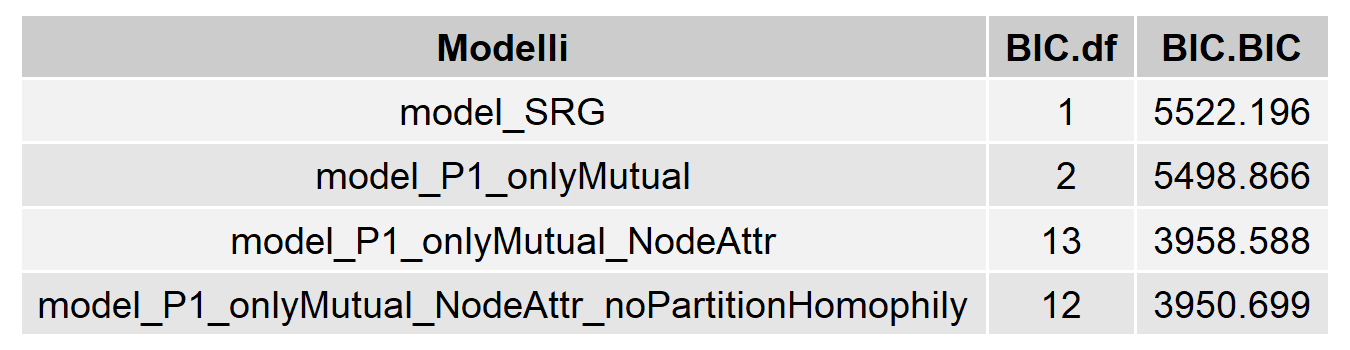
\includegraphics{images/SRG_and_P1_Models_BIC.png}

    ``model\_P1\_onlyMutual\_NodeAttr'' e
``model\_P1\_onlyMutual\_NodeAttr\_noPartitionHomophily'' sono i due
modelli migliori e differiscono tra di loro di veramente pochi punti,
ragion per cui per decidere il miglior modello P1 confronteremo
l'abilità di questi modelli nel simulare le statistiche di rete e le
statistiche nodali.

    \begin{tcolorbox}[breakable, size=fbox, boxrule=1pt, pad at break*=1mm,colback=cellbackground, colframe=cellborder]
\prompt{In}{incolor}{34}{\boxspacing}
\begin{Verbatim}[commandchars=\\\{\}]
\PY{n}{sim1}\PY{+w}{ }\PY{o}{\PYZlt{}\PYZhy{}}\PY{+w}{ }\PY{n+nf}{suppressMessages}\PY{p}{(}\PY{n+nf}{simulate}\PY{p}{(}\PY{n}{model\PYZus{}P1\PYZus{}onlyMutual\PYZus{}NodeAttr}\PY{p}{,}\PY{+w}{ }\PY{n}{nsim}\PY{+w}{ }\PY{o}{=}\PY{+w}{ }\PY{l+m}{100}\PY{p}{,}\PY{+w}{ }\PY{n}{verbose}\PY{+w}{ }\PY{o}{=}\PY{+w}{ }\PY{k+kc}{TRUE}\PY{p}{,}\PY{+w}{ }\PY{n}{seed}\PY{+w}{ }\PY{o}{=}\PY{+w}{ }\PY{l+m}{1}\PY{p}{)}\PY{p}{)}

\PY{n}{null.distr1}\PY{+w}{ }\PY{o}{\PYZlt{}\PYZhy{}}\PY{+w}{ }\PY{n+nf}{matrix}\PY{p}{(}\PY{p}{,}\PY{l+m}{100}\PY{p}{,}\PY{l+m}{4}\PY{p}{)}
\PY{n+nf}{for}\PY{p}{(}\PY{n}{b}\PY{+w}{ }\PY{n}{in}\PY{+w}{ }\PY{l+m}{1}\PY{o}{:}\PY{l+m}{100}\PY{p}{)}\PY{p}{\PYZob{}}
\PY{+w}{	}\PY{n}{null.distr1}\PY{p}{[}\PY{n}{b}\PY{p}{,}\PY{p}{]}\PY{+w}{ }\PY{o}{\PYZlt{}\PYZhy{}}\PY{+w}{ }\PY{n+nf}{extractInformationsFromGraph}\PY{p}{(}\PY{n}{sim1}\PY{p}{[[}\PY{n}{b}\PY{p}{]]}\PY{p}{)}
\PY{p}{\PYZcb{}}

\PY{n}{sim2}\PY{+w}{ }\PY{o}{\PYZlt{}\PYZhy{}}\PY{+w}{ }\PY{n+nf}{suppressMessages}\PY{p}{(}\PY{p}{(}\PY{n+nf}{simulate}\PY{p}{(}\PY{n}{model\PYZus{}P1\PYZus{}onlyMutual\PYZus{}NodeAttr\PYZus{}noPartitionHomophily}\PY{p}{,}\PY{+w}{ }\PY{n}{nsim}\PY{+w}{ }\PY{o}{=}\PY{+w}{ }\PY{l+m}{100}\PY{p}{,}\PY{+w}{ }\PY{n}{verbose}\PY{+w}{ }\PY{o}{=}\PY{+w}{ }\PY{k+kc}{TRUE}\PY{p}{,}\PY{+w}{ }\PY{n}{seed}\PY{+w}{ }\PY{o}{=}\PY{+w}{ }\PY{l+m}{1}\PY{p}{)}\PY{p}{)}\PY{p}{)}

\PY{n}{null.distr2}\PY{+w}{ }\PY{o}{\PYZlt{}\PYZhy{}}\PY{+w}{ }\PY{n+nf}{matrix}\PY{p}{(}\PY{p}{,}\PY{l+m}{100}\PY{p}{,}\PY{l+m}{4}\PY{p}{)}
\PY{n+nf}{for}\PY{p}{(}\PY{n}{b}\PY{+w}{ }\PY{n}{in}\PY{+w}{ }\PY{l+m}{1}\PY{o}{:}\PY{l+m}{100}\PY{p}{)}\PY{p}{\PYZob{}}
\PY{+w}{	}\PY{n}{null.distr2}\PY{p}{[}\PY{n}{b}\PY{p}{,}\PY{p}{]}\PY{+w}{ }\PY{o}{\PYZlt{}\PYZhy{}}\PY{+w}{ }\PY{n+nf}{extractInformationsFromGraph}\PY{p}{(}\PY{n}{sim2}\PY{p}{[[}\PY{n}{b}\PY{p}{]]}\PY{p}{)}
\PY{p}{\PYZcb{}}
\end{Verbatim}
\end{tcolorbox}

    \begin{tcolorbox}[breakable, size=fbox, boxrule=1pt, pad at break*=1mm,colback=cellbackground, colframe=cellborder]
\prompt{In}{incolor}{35}{\boxspacing}
\begin{Verbatim}[commandchars=\\\{\}]
\PY{n+nf}{png}\PY{p}{(}\PY{l+s}{\PYZdq{}}\PY{l+s}{images/model\PYZus{}P1\PYZus{}onlyMutual\PYZus{}NodeAttr\PYZus{}VS\PYZus{}model\PYZus{}P1\PYZus{}onlyMutual\PYZus{}NodeAttr\PYZus{}noPartitionHomophily\PYZus{}\PYZus{}Part1.png\PYZdq{}}\PY{p}{,}\PY{+w}{ }\PY{n}{width}\PY{+w}{ }\PY{o}{=}\PY{+w}{ }\PY{l+m}{1000}\PY{p}{,}\PY{+w}{ }\PY{n}{height}\PY{+w}{ }\PY{o}{=}\PY{+w}{ }\PY{l+m}{1000}\PY{p}{,}\PY{+w}{ }\PY{n}{res}\PY{+w}{ }\PY{o}{=}\PY{+w}{ }\PY{l+m}{150}\PY{p}{)}
\PY{n+nf}{par}\PY{p}{(}\PY{n}{mfrow}\PY{+w}{ }\PY{o}{=}\PY{+w}{ }\PY{n+nf}{c}\PY{p}{(}\PY{l+m}{4}\PY{p}{,}\PY{l+m}{1}\PY{p}{)}\PY{p}{)}
\PY{n+nf}{hist}\PY{p}{(}\PY{n+nf}{unlist}\PY{p}{(}\PY{n}{null.distr1}\PY{p}{[}\PY{p}{,}\PY{l+m}{2}\PY{p}{]}\PY{p}{)}\PY{p}{,}\PY{+w}{ }\PY{n}{xlab}\PY{+w}{ }\PY{o}{=}\PY{+w}{ }\PY{l+s}{\PYZdq{}}\PY{l+s}{in\PYZhy{}degree\PYZdq{}}\PY{p}{,}\PY{+w}{ }\PY{n}{xlim}\PY{+w}{ }\PY{o}{=}\PY{+w}{ }\PY{n+nf}{c}\PY{p}{(}\PY{l+m}{2}\PY{p}{,}\PY{l+m}{12}\PY{p}{)}\PY{p}{,}\PY{+w}{ }\PY{n}{main}\PY{+w}{ }\PY{o}{=}\PY{+w}{ }\PY{l+s}{\PYZdq{}}\PY{l+s}{In Degree Distribution with Partition Homophily\PYZdq{}}\PY{p}{)}\PY{p}{;}\PY{+w}{ }\PY{n+nf}{abline}\PY{p}{(}\PY{n}{v}\PY{+w}{ }\PY{o}{=}\PY{+w}{ }\PY{n+nf}{sd}\PY{p}{(}\PY{n+nf}{degree}\PY{p}{(}\PY{n}{g}\PY{p}{,}\PY{+w}{ }\PY{n}{mode}\PY{+w}{ }\PY{o}{=}\PY{+w}{ }\PY{l+s}{\PYZdq{}}\PY{l+s}{in\PYZdq{}}\PY{p}{)}\PY{p}{)}\PY{p}{,}\PY{+w}{ }\PY{n}{col}\PY{+w}{ }\PY{o}{=}\PY{+w}{ }\PY{l+s}{\PYZdq{}}\PY{l+s}{red\PYZdq{}}\PY{p}{)}
\PY{n+nf}{hist}\PY{p}{(}\PY{n+nf}{unlist}\PY{p}{(}\PY{n}{null.distr2}\PY{p}{[}\PY{p}{,}\PY{l+m}{2}\PY{p}{]}\PY{p}{)}\PY{p}{,}\PY{+w}{ }\PY{n}{xlab}\PY{+w}{ }\PY{o}{=}\PY{+w}{ }\PY{l+s}{\PYZdq{}}\PY{l+s}{in\PYZhy{}degree\PYZdq{}}\PY{p}{,}\PY{+w}{ }\PY{n}{xlim}\PY{+w}{ }\PY{o}{=}\PY{+w}{ }\PY{n+nf}{c}\PY{p}{(}\PY{l+m}{2}\PY{p}{,}\PY{l+m}{12}\PY{p}{)}\PY{p}{,}\PY{+w}{ }\PY{n}{main}\PY{+w}{ }\PY{o}{=}\PY{+w}{ }\PY{l+s}{\PYZdq{}}\PY{l+s}{In Degree Distribution without Partition Homophily\PYZdq{}}\PY{p}{)}\PY{p}{;}\PY{+w}{ }\PY{n+nf}{abline}\PY{p}{(}\PY{n}{v}\PY{+w}{ }\PY{o}{=}\PY{+w}{ }\PY{n+nf}{sd}\PY{p}{(}\PY{n+nf}{degree}\PY{p}{(}\PY{n}{g}\PY{p}{,}\PY{+w}{ }\PY{n}{mode}\PY{+w}{ }\PY{o}{=}\PY{+w}{ }\PY{l+s}{\PYZdq{}}\PY{l+s}{in\PYZdq{}}\PY{p}{)}\PY{p}{)}\PY{p}{,}\PY{+w}{ }\PY{n}{col}\PY{+w}{ }\PY{o}{=}\PY{+w}{ }\PY{l+s}{\PYZdq{}}\PY{l+s}{red\PYZdq{}}\PY{p}{)}
\PY{n+nf}{hist}\PY{p}{(}\PY{n+nf}{unlist}\PY{p}{(}\PY{n}{null.distr1}\PY{p}{[}\PY{p}{,}\PY{l+m}{3}\PY{p}{]}\PY{p}{)}\PY{p}{,}\PY{+w}{ }\PY{n}{xlab}\PY{+w}{ }\PY{o}{=}\PY{+w}{ }\PY{l+s}{\PYZdq{}}\PY{l+s}{out\PYZhy{}degree\PYZdq{}}\PY{p}{,}\PY{+w}{ }\PY{n}{xlim}\PY{o}{=}\PY{n+nf}{c}\PY{p}{(}\PY{l+m}{5}\PY{p}{,}\PY{+w}{ }\PY{l+m}{22}\PY{p}{)}\PY{p}{,}\PY{+w}{ }\PY{n}{main}\PY{+w}{ }\PY{o}{=}\PY{+w}{ }\PY{l+s}{\PYZdq{}}\PY{l+s}{Out Degree Distribution with Partition Homophily\PYZdq{}}\PY{p}{)}\PY{p}{;}\PY{+w}{ }\PY{n+nf}{abline}\PY{p}{(}\PY{n}{v}\PY{+w}{ }\PY{o}{=}\PY{+w}{ }\PY{n+nf}{sd}\PY{p}{(}\PY{n+nf}{degree}\PY{p}{(}\PY{n}{g}\PY{p}{,}\PY{+w}{ }\PY{n}{mode}\PY{+w}{ }\PY{o}{=}\PY{+w}{ }\PY{l+s}{\PYZdq{}}\PY{l+s}{out\PYZdq{}}\PY{p}{)}\PY{p}{)}\PY{p}{,}\PY{+w}{ }\PY{n}{col}\PY{+w}{ }\PY{o}{=}\PY{+w}{ }\PY{l+s}{\PYZdq{}}\PY{l+s}{red\PYZdq{}}\PY{p}{)}
\PY{n+nf}{hist}\PY{p}{(}\PY{n+nf}{unlist}\PY{p}{(}\PY{n}{null.distr2}\PY{p}{[}\PY{p}{,}\PY{l+m}{3}\PY{p}{]}\PY{p}{)}\PY{p}{,}\PY{+w}{ }\PY{n}{xlab}\PY{+w}{ }\PY{o}{=}\PY{+w}{ }\PY{l+s}{\PYZdq{}}\PY{l+s}{out\PYZhy{}degree\PYZdq{}}\PY{p}{,}\PY{+w}{ }\PY{n}{xlim}\PY{o}{=}\PY{n+nf}{c}\PY{p}{(}\PY{l+m}{5}\PY{p}{,}\PY{+w}{ }\PY{l+m}{22}\PY{p}{)}\PY{p}{,}\PY{+w}{ }\PY{n}{main}\PY{+w}{ }\PY{o}{=}\PY{+w}{ }\PY{l+s}{\PYZdq{}}\PY{l+s}{Out Degree Distribution without Partition Homophily\PYZdq{}}\PY{p}{)}\PY{p}{;}\PY{+w}{ }\PY{n+nf}{abline}\PY{p}{(}\PY{n}{v}\PY{+w}{ }\PY{o}{=}\PY{+w}{ }\PY{n+nf}{sd}\PY{p}{(}\PY{n+nf}{degree}\PY{p}{(}\PY{n}{g}\PY{p}{,}\PY{+w}{ }\PY{n}{mode}\PY{+w}{ }\PY{o}{=}\PY{+w}{ }\PY{l+s}{\PYZdq{}}\PY{l+s}{out\PYZdq{}}\PY{p}{)}\PY{p}{)}\PY{p}{,}\PY{+w}{ }\PY{n}{col}\PY{+w}{ }\PY{o}{=}\PY{+w}{ }\PY{l+s}{\PYZdq{}}\PY{l+s}{red\PYZdq{}}\PY{p}{)}
\PY{n+nf}{invisible}\PY{p}{(}\PY{n+nf}{dev.off}\PY{p}{(}\PY{p}{)}\PY{p}{)}

\PY{n+nf}{png}\PY{p}{(}\PY{l+s}{\PYZdq{}}\PY{l+s}{images/model\PYZus{}P1\PYZus{}onlyMutual\PYZus{}NodeAttr\PYZus{}VS\PYZus{}model\PYZus{}P1\PYZus{}onlyMutual\PYZus{}NodeAttr\PYZus{}noPartitionHomophily\PYZus{}\PYZus{}Part2.png\PYZdq{}}\PY{p}{,}\PY{+w}{ }\PY{n}{width}\PY{+w}{ }\PY{o}{=}\PY{+w}{ }\PY{l+m}{1000}\PY{p}{,}\PY{+w}{ }\PY{n}{height}\PY{+w}{ }\PY{o}{=}\PY{+w}{ }\PY{l+m}{1000}\PY{p}{,}\PY{+w}{ }\PY{n}{res}\PY{+w}{ }\PY{o}{=}\PY{+w}{ }\PY{l+m}{150}\PY{p}{)}
\PY{n+nf}{par}\PY{p}{(}\PY{n}{mfrow}\PY{+w}{ }\PY{o}{=}\PY{+w}{ }\PY{n+nf}{c}\PY{p}{(}\PY{l+m}{4}\PY{p}{,}\PY{l+m}{1}\PY{p}{)}\PY{p}{)}
\PY{n+nf}{hist}\PY{p}{(}\PY{n+nf}{unlist}\PY{p}{(}\PY{n}{null.distr1}\PY{p}{[}\PY{p}{,}\PY{l+m}{1}\PY{p}{]}\PY{p}{)}\PY{p}{,}\PY{+w}{ }\PY{n}{xlab}\PY{+w}{ }\PY{o}{=}\PY{+w}{ }\PY{l+s}{\PYZdq{}}\PY{l+s}{transitivity\PYZdq{}}\PY{p}{,}\PY{+w}{ }\PY{n}{xlim}\PY{o}{=}\PY{n+nf}{c}\PY{p}{(}\PY{l+m}{0.4}\PY{p}{,}\PY{+w}{ }\PY{l+m}{0.5}\PY{p}{)}\PY{p}{,}\PY{+w}{ }\PY{n}{main}\PY{+w}{ }\PY{o}{=}\PY{+w}{ }\PY{l+s}{\PYZdq{}}\PY{l+s}{Transitivity Distribution with Partition Homophily\PYZdq{}}\PY{p}{)}\PY{p}{;}\PY{+w}{ }\PY{n+nf}{abline}\PY{p}{(}\PY{n}{v}\PY{+w}{ }\PY{o}{=}\PY{+w}{ }\PY{n+nf}{transitivity}\PY{p}{(}\PY{n}{g}\PY{p}{)}\PY{p}{,}\PY{+w}{ }\PY{n}{col}\PY{+w}{ }\PY{o}{=}\PY{+w}{ }\PY{l+s}{\PYZdq{}}\PY{l+s}{red\PYZdq{}}\PY{p}{)}
\PY{n+nf}{hist}\PY{p}{(}\PY{n+nf}{unlist}\PY{p}{(}\PY{n}{null.distr2}\PY{p}{[}\PY{p}{,}\PY{l+m}{1}\PY{p}{]}\PY{p}{)}\PY{p}{,}\PY{+w}{ }\PY{n}{xlab}\PY{+w}{ }\PY{o}{=}\PY{+w}{ }\PY{l+s}{\PYZdq{}}\PY{l+s}{transitivity\PYZdq{}}\PY{p}{,}\PY{+w}{ }\PY{n}{xlim}\PY{o}{=}\PY{n+nf}{c}\PY{p}{(}\PY{l+m}{0.4}\PY{p}{,}\PY{+w}{ }\PY{l+m}{0.5}\PY{p}{)}\PY{p}{,}\PY{+w}{ }\PY{n}{main}\PY{+w}{ }\PY{o}{=}\PY{+w}{ }\PY{l+s}{\PYZdq{}}\PY{l+s}{Transitivity Distribution without Partition Homophily\PYZdq{}}\PY{p}{)}\PY{p}{;}\PY{+w}{ }\PY{n+nf}{abline}\PY{p}{(}\PY{n}{v}\PY{+w}{ }\PY{o}{=}\PY{+w}{ }\PY{n+nf}{transitivity}\PY{p}{(}\PY{n}{g}\PY{p}{)}\PY{p}{,}\PY{+w}{ }\PY{n}{col}\PY{+w}{ }\PY{o}{=}\PY{+w}{ }\PY{l+s}{\PYZdq{}}\PY{l+s}{red\PYZdq{}}\PY{p}{)}
\PY{n+nf}{hist}\PY{p}{(}\PY{n+nf}{unlist}\PY{p}{(}\PY{n}{null.distr1}\PY{p}{[}\PY{p}{,}\PY{l+m}{4}\PY{p}{]}\PY{p}{)}\PY{p}{,}\PY{+w}{ }\PY{n}{xlab}\PY{+w}{ }\PY{o}{=}\PY{+w}{ }\PY{l+s}{\PYZdq{}}\PY{l+s}{density\PYZdq{}}\PY{p}{,}\PY{+w}{ }\PY{n}{main}\PY{+w}{ }\PY{o}{=}\PY{+w}{ }\PY{l+s}{\PYZdq{}}\PY{l+s}{Density Distribution with Partition Homophily\PYZdq{}}\PY{p}{)}\PY{p}{;}\PY{+w}{ }\PY{n+nf}{abline}\PY{p}{(}\PY{n}{v}\PY{+w}{ }\PY{o}{=}\PY{+w}{ }\PY{n+nf}{edge\PYZus{}density}\PY{p}{(}\PY{n}{g}\PY{p}{)}\PY{p}{,}\PY{+w}{ }\PY{n}{col}\PY{+w}{ }\PY{o}{=}\PY{+w}{ }\PY{l+s}{\PYZdq{}}\PY{l+s}{red\PYZdq{}}\PY{p}{)}
\PY{n+nf}{hist}\PY{p}{(}\PY{n+nf}{unlist}\PY{p}{(}\PY{n}{null.distr2}\PY{p}{[}\PY{p}{,}\PY{l+m}{4}\PY{p}{]}\PY{p}{)}\PY{p}{,}\PY{+w}{ }\PY{n}{xlab}\PY{+w}{ }\PY{o}{=}\PY{+w}{ }\PY{l+s}{\PYZdq{}}\PY{l+s}{density\PYZdq{}}\PY{p}{,}\PY{+w}{ }\PY{n}{main}\PY{+w}{ }\PY{o}{=}\PY{+w}{ }\PY{l+s}{\PYZdq{}}\PY{l+s}{Density Distribution without Partition Homophily\PYZdq{}}\PY{p}{)}\PY{p}{;}\PY{+w}{ }\PY{n+nf}{abline}\PY{p}{(}\PY{n}{v}\PY{+w}{ }\PY{o}{=}\PY{+w}{ }\PY{n+nf}{edge\PYZus{}density}\PY{p}{(}\PY{n}{g}\PY{p}{)}\PY{p}{,}\PY{+w}{ }\PY{n}{col}\PY{+w}{ }\PY{o}{=}\PY{+w}{ }\PY{l+s}{\PYZdq{}}\PY{l+s}{red\PYZdq{}}\PY{p}{)}
\PY{n+nf}{invisible}\PY{p}{(}\PY{n+nf}{dev.off}\PY{p}{(}\PY{p}{)}\PY{p}{)}
\end{Verbatim}
\end{tcolorbox}

    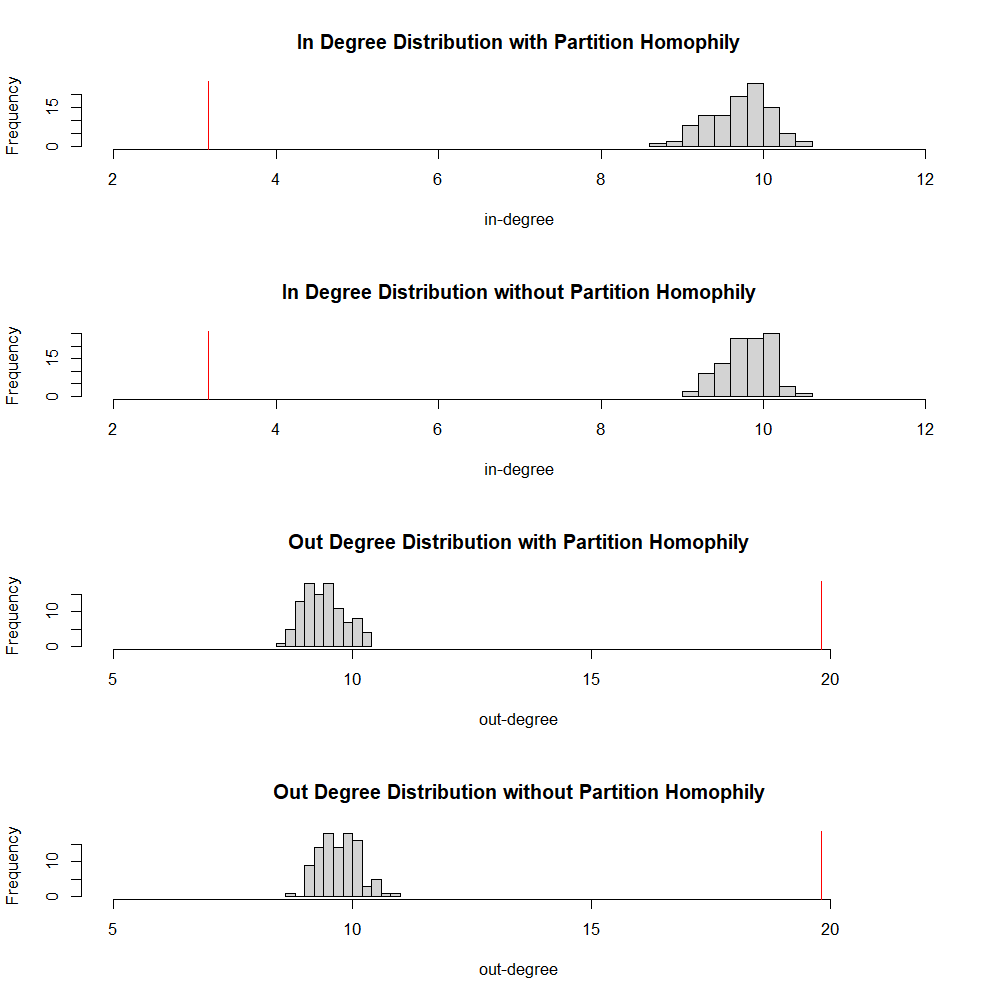
\includegraphics{images/model_P1_onlyMutual_NodeAttr_VS_model_P1_onlyMutual_NodeAttr_noPartitionHomophily__Part1.png}

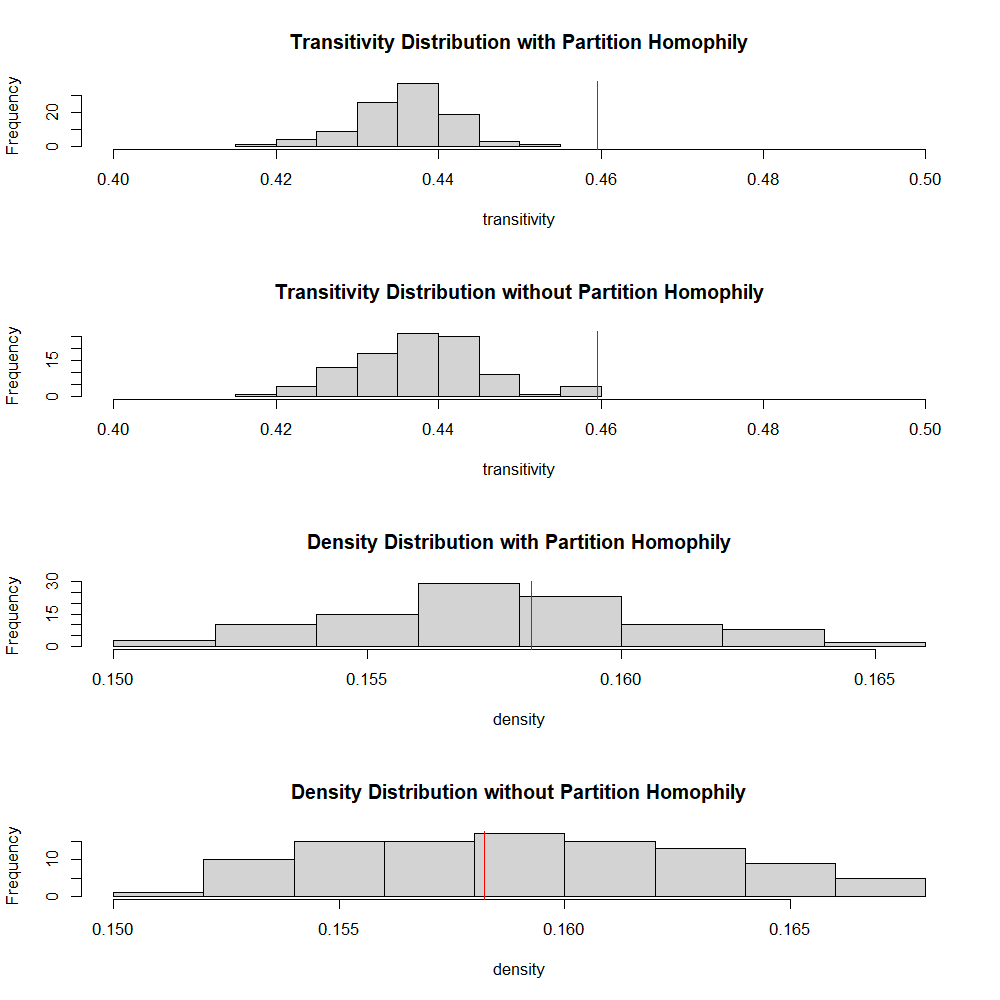
\includegraphics{images/model_P1_onlyMutual_NodeAttr_VS_model_P1_onlyMutual_NodeAttr_noPartitionHomophily__Part2.png}

    Apparentemente dai metodi di valutazione AIC e BIC viene da pensare che
questi ultimi due modelli siano migliori del modello SRG ma a quanto
pare perdiamo la capacità di catturare la In-Degree della nostra Rete.

    \subsubsection{Markov Graph Model}\label{markov-graph-model}

Poi abbiamo provato a generare modelli di Markov, ma sfortunatamente
molti di essi hanno dato Degeneracy Problems.

L'unico modello di Markov che siamo riusciti a calcolare è stato il
modello che utilizzava soltanto le 2 Star in Input.

    \begin{tcolorbox}[breakable, size=fbox, boxrule=1pt, pad at break*=1mm,colback=cellbackground, colframe=cellborder]
\prompt{In}{incolor}{36}{\boxspacing}
\begin{Verbatim}[commandchars=\\\{\}]
\PY{n+nf}{summary}\PY{p}{(}\PY{n}{model\PYZus{}Markov\PYZus{}onlyIStar2}\PY{p}{)}
\end{Verbatim}
\end{tcolorbox}

    
    \begin{Verbatim}[commandchars=\\\{\}]
Call:
ergm(formula = net \textasciitilde{} edges + mutual + nodecov("gdp") + nodefactor("continent") + 
    nodefactor("partition") + absdiff("gdp") + nodematch("continent") + 
    nodematch("partition") + istar(2), control = control.ergm(seed = 1, 
    checkpoint = "mod3\_onlyIStar2/step\_\%03d.RData"))

Monte Carlo Maximum Likelihood Results:

                         Estimate Std. Error MCMC \% z value Pr(>|z|)    
edges                   7.810e+00  5.413e-01      0  14.429  < 1e-04 ***
mutual                 -1.002e+00  1.923e-01      0  -5.212  < 1e-04 ***
nodecov.gdp             1.382e-05  5.058e-06      0   2.733  0.00628 ** 
nodefactor.continent.2  2.519e-01  1.684e-01      0   1.496  0.13461    
nodefactor.continent.3 -3.721e-01  1.718e-01      0  -2.166  0.03027 *  
nodefactor.continent.4  1.652e+00  2.226e-01      0   7.423  < 1e-04 ***
nodefactor.continent.5  1.079e+00  2.653e-01      0   4.067  < 1e-04 ***
nodefactor.continent.6  8.533e-02  1.771e-01      0   0.482  0.62992    
nodefactor.partition.2 -3.309e+00  1.575e-01      0 -21.006  < 1e-04 ***
nodefactor.partition.3 -5.518e+00  2.456e-01      0 -22.473  < 1e-04 ***
absdiff.gdp            -2.757e-05  5.550e-06      0  -4.967  < 1e-04 ***
nodematch.continent     2.236e+00  1.229e-01      0  18.199  < 1e-04 ***
nodematch.partition    -2.008e-01  1.349e-01      0  -1.488  0.13667    
istar2                 -3.572e-01  3.157e-02      0 -11.315  < 1e-04 ***
---
Signif. codes:  0 '***' 0.001 '**' 0.01 '*' 0.05 '.' 0.1 ' ' 1

     Null Deviance: 8761  on 6320  degrees of freedom
 Residual Deviance: 3404  on 6306  degrees of freedom
 
AIC: 3432  BIC: 3527  (Smaller is better. MC Std. Err. = 3.166)
    \end{Verbatim}

    
    Dal summary possiamo notare che l'effetto di omofilia rispetto alla
partizione non è significativa, quindi possiamo provare a ricalcolare il
modello togliendo tale effetto e verificare se questo migliori oppure no

    \begin{tcolorbox}[breakable, size=fbox, boxrule=1pt, pad at break*=1mm,colback=cellbackground, colframe=cellborder]
\prompt{In}{incolor}{37}{\boxspacing}
\begin{Verbatim}[commandchars=\\\{\}]
\PY{n+nf}{summary}\PY{p}{(}\PY{n}{model\PYZus{}Markov\PYZus{}onlyIStar2\PYZus{}noPartitionHomophily}\PY{p}{)}
\end{Verbatim}
\end{tcolorbox}

    
    \begin{Verbatim}[commandchars=\\\{\}]
Call:
ergm(formula = net \textasciitilde{} edges + mutual + nodecov("gdp") + nodefactor("continent") + 
    nodefactor("partition") + absdiff("gdp") + nodematch("continent") + 
    istar(2), control = control.ergm(seed = 1))

Monte Carlo Maximum Likelihood Results:

                         Estimate Std. Error MCMC \% z value Pr(>|z|)    
edges                   7.849e+00  5.324e-01      0  14.744  < 1e-04 ***
mutual                 -1.002e+00  1.959e-01      0  -5.113  < 1e-04 ***
nodecov.gdp             1.365e-05  5.215e-06      0   2.617  0.00888 ** 
nodefactor.continent.2  2.616e-01  1.669e-01      0   1.568  0.11699    
nodefactor.continent.3 -3.625e-01  1.716e-01      0  -2.112  0.03465 *  
nodefactor.continent.4  1.645e+00  2.208e-01      0   7.451  < 1e-04 ***
nodefactor.continent.5  1.073e+00  2.670e-01      0   4.019  < 1e-04 ***
nodefactor.continent.6  8.907e-02  1.746e-01      0   0.510  0.60988    
nodefactor.partition.2 -3.405e+00  1.396e-01      0 -24.391  < 1e-04 ***
nodefactor.partition.3 -5.521e+00  2.440e-01      0 -22.627  < 1e-04 ***
absdiff.gdp            -2.659e-05  5.517e-06      0  -4.819  < 1e-04 ***
nodematch.continent     2.207e+00  1.196e-01      0  18.453  < 1e-04 ***
istar2                 -3.585e-01  3.106e-02      0 -11.542  < 1e-04 ***
---
Signif. codes:  0 '***' 0.001 '**' 0.01 '*' 0.05 '.' 0.1 ' ' 1

     Null Deviance: 8761  on 6320  degrees of freedom
 Residual Deviance: 3398  on 6307  degrees of freedom
 
AIC: 3424  BIC: 3511  (Smaller is better. MC Std. Err. = 3.975)
    \end{Verbatim}

    
    Poi abbiamo provato ad utilizzare la variante delle Alternating K-Star
per ridurre la probabilità che i modelli di Markov degenerasserò,
sfortunatamente però alcuni modelli hanno comunque dato problemi di
degenerazione. Siamo stati in grado di calcolare solo due modelli:

\begin{itemize}
\tightlist
\item
  Il primo modello tiene in considerazione le Alternating K-Star in
  Ingresso (model\_Markov\_onlyAlterantingInKStar)
\item
  Il secondo modello tiene in considerazione le Alternating K-Star in
  Uscita (model\_Markov\_onlyAlternatingOutKStar)
\end{itemize}

    \begin{tcolorbox}[breakable, size=fbox, boxrule=1pt, pad at break*=1mm,colback=cellbackground, colframe=cellborder]
\prompt{In}{incolor}{38}{\boxspacing}
\begin{Verbatim}[commandchars=\\\{\}]
\PY{n+nf}{summary}\PY{p}{(}\PY{n}{model\PYZus{}Markov\PYZus{}onlyAlternatingInKStar}\PY{p}{)}
\end{Verbatim}
\end{tcolorbox}

    
    \begin{Verbatim}[commandchars=\\\{\}]
Call:
ergm(formula = net \textasciitilde{} edges + mutual + nodecov("gdp") + nodefactor("continent") + 
    nodefactor("partition") + absdiff("gdp") + nodematch("continent") + 
    nodematch("partition") + +gwidegree(decay = 1, fixed = TRUE), 
    control = control.ergm(seed = 1))

Monte Carlo Maximum Likelihood Results:

                         Estimate Std. Error MCMC \% z value Pr(>|z|)    
edges                   2.353e+00  3.952e-01      0   5.955   <1e-04 ***
mutual                 -1.759e+00  1.827e-01      0  -9.629   <1e-04 ***
nodecov.gdp             1.222e-05  4.826e-06      0   2.532   0.0113 *  
nodefactor.continent.2  2.153e-01  1.604e-01      0   1.342   0.1797    
nodefactor.continent.3 -3.934e-01  1.668e-01      0  -2.358   0.0184 *  
nodefactor.continent.4  1.459e+00  2.107e-01      0   6.926   <1e-04 ***
nodefactor.continent.5  1.007e+00  2.577e-01      0   3.908   <1e-04 ***
nodefactor.continent.6  5.868e-02  1.744e-01      0   0.337   0.7365    
nodefactor.partition.2 -3.022e+00  1.570e-01      0 -19.245   <1e-04 ***
nodefactor.partition.3 -5.065e+00  2.419e-01      0 -20.937   <1e-04 ***
absdiff.gdp            -2.561e-05  5.554e-06      0  -4.611   <1e-04 ***
nodematch.continent     2.250e+00  1.242e-01      0  18.122   <1e-04 ***
nodematch.partition    -1.546e-01  1.357e-01      0  -1.139   0.2546    
gwideg.fixed.1          6.138e+01  7.741e+00      0   7.930   <1e-04 ***
---
Signif. codes:  0 '***' 0.001 '**' 0.01 '*' 0.05 '.' 0.1 ' ' 1

     Null Deviance: 8761  on 6320  degrees of freedom
 Residual Deviance: 3684  on 6306  degrees of freedom
 
AIC: 3712  BIC: 3807  (Smaller is better. MC Std. Err. = 1.53)
    \end{Verbatim}

    
    \begin{tcolorbox}[breakable, size=fbox, boxrule=1pt, pad at break*=1mm,colback=cellbackground, colframe=cellborder]
\prompt{In}{incolor}{39}{\boxspacing}
\begin{Verbatim}[commandchars=\\\{\}]
\PY{n+nf}{summary}\PY{p}{(}\PY{n}{model\PYZus{}Markov\PYZus{}onlyAlternatingOutKStar}\PY{p}{)}
\end{Verbatim}
\end{tcolorbox}

    
    \begin{Verbatim}[commandchars=\\\{\}]
Call:
ergm(formula = net \textasciitilde{} edges + mutual + nodecov("gdp") + nodefactor("continent") + 
    nodefactor("partition") + absdiff("gdp") + nodematch("continent") + 
    nodematch("partition") + +gwodegree(decay = 1, fixed = TRUE), 
    control = control.ergm(seed = 1), verbose = 3)

Monte Carlo Maximum Likelihood Results:

                         Estimate Std. Error MCMC \% z value Pr(>|z|)    
edges                   3.548e+00  2.707e-01      0  13.107  < 1e-04 ***
mutual                 -1.616e+00  1.798e-01      0  -8.985  < 1e-04 ***
nodecov.gdp             5.457e-06  2.979e-06      0   1.832 0.066966 .  
nodefactor.continent.2 -2.627e-01  7.186e-02      0  -3.655 0.000257 ***
nodefactor.continent.3 -7.824e-01  8.143e-02      0  -9.609  < 1e-04 ***
nodefactor.continent.4  5.782e-01  1.295e-01      0   4.463  < 1e-04 ***
nodefactor.continent.5  4.714e-01  1.453e-01      0   3.244 0.001178 ** 
nodefactor.continent.6 -1.768e-01  7.481e-02      0  -2.363 0.018131 *  
nodefactor.partition.2 -2.605e+00  1.469e-01      0 -17.730  < 1e-04 ***
nodefactor.partition.3 -3.353e+00  1.866e-01      0 -17.970  < 1e-04 ***
absdiff.gdp            -2.128e-05  5.400e-06      0  -3.941  < 1e-04 ***
nodematch.continent     2.500e+00  1.287e-01      0  19.421  < 1e-04 ***
nodematch.partition    -2.509e-01  1.434e-01      0  -1.750 0.080126 .  
gwodeg.fixed.1         -6.408e+00  2.510e-01      0 -25.530  < 1e-04 ***
---
Signif. codes:  0 '***' 0.001 '**' 0.01 '*' 0.05 '.' 0.1 ' ' 1

     Null Deviance: 8761  on 6320  degrees of freedom
 Residual Deviance: 3199  on 6306  degrees of freedom
 
AIC: 3227  BIC: 3321  (Smaller is better. MC Std. Err. = 0.9433)
    \end{Verbatim}

    
    Dai dati sopra possiamo notare come:

\begin{itemize}
\tightlist
\item
  Il primo modello risulta dare poca significatività all'effetto di
  omofilia della Partizione
\item
  Il secondo modello risulta dare poca significatività all'effetto
  principale dell'attributo GDP e all'effetto di omofilia della
  Partizione
\end{itemize}

Possiamo provare a rimuovere tali effetti dai modelli e verificare se
sussiste un miglioramento dei modelli oppure no

    \begin{tcolorbox}[breakable, size=fbox, boxrule=1pt, pad at break*=1mm,colback=cellbackground, colframe=cellborder]
\prompt{In}{incolor}{40}{\boxspacing}
\begin{Verbatim}[commandchars=\\\{\}]
\PY{n+nf}{summary}\PY{p}{(}\PY{n}{model\PYZus{}Markov\PYZus{}onlyAlternatingInKStar\PYZus{}noPartitionHomophily}\PY{p}{)}
\end{Verbatim}
\end{tcolorbox}

    
    \begin{Verbatim}[commandchars=\\\{\}]
Call:
ergm(formula = net \textasciitilde{} edges + mutual + nodecov("gdp") + nodefactor("continent") + 
    nodefactor("partition") + absdiff("gdp") + nodematch("continent") + 
    gwidegree(decay = 1, fixed = TRUE), control = control.ergm(seed = 1))

Monte Carlo Maximum Likelihood Results:

                         Estimate Std. Error MCMC \% z value Pr(>|z|)    
edges                   2.399e+00  3.964e-01      0   6.052  < 1e-04 ***
mutual                 -1.756e+00  1.810e-01      0  -9.703  < 1e-04 ***
nodecov.gdp             1.209e-05  4.717e-06      0   2.564 0.010361 *  
nodefactor.continent.2  2.149e-01  1.627e-01      0   1.321 0.186506    
nodefactor.continent.3 -3.838e-01  1.685e-01      0  -2.278 0.022718 *  
nodefactor.continent.4  1.450e+00  2.147e-01      0   6.756  < 1e-04 ***
nodefactor.continent.5  9.971e-01  2.615e-01      0   3.813 0.000137 ***
nodefactor.continent.6  6.639e-02  1.783e-01      0   0.372 0.709680    
nodefactor.partition.2 -3.105e+00  1.347e-01      0 -23.049  < 1e-04 ***
nodefactor.partition.3 -5.101e+00  2.359e-01      0 -21.622  < 1e-04 ***
absdiff.gdp            -2.491e-05  5.554e-06      0  -4.485  < 1e-04 ***
nodematch.continent     2.229e+00  1.217e-01      0  18.308  < 1e-04 ***
gwideg.fixed.1          6.106e+01  7.742e+00      0   7.887  < 1e-04 ***
---
Signif. codes:  0 '***' 0.001 '**' 0.01 '*' 0.05 '.' 0.1 ' ' 1

     Null Deviance: 8761  on 6320  degrees of freedom
 Residual Deviance: 3686  on 6307  degrees of freedom
 
AIC: 3712  BIC: 3800  (Smaller is better. MC Std. Err. = 0.9847)
    \end{Verbatim}

    
    \begin{tcolorbox}[breakable, size=fbox, boxrule=1pt, pad at break*=1mm,colback=cellbackground, colframe=cellborder]
\prompt{In}{incolor}{41}{\boxspacing}
\begin{Verbatim}[commandchars=\\\{\}]
\PY{n+nf}{summary}\PY{p}{(}\PY{n}{model\PYZus{}Markov\PYZus{}onlyAlternatingOutKStar\PYZus{}noPartitionHomophily\PYZus{}noGDPMain}\PY{p}{)}
\end{Verbatim}
\end{tcolorbox}

    
    \begin{Verbatim}[commandchars=\\\{\}]
Call:
ergm(formula = net \textasciitilde{} edges + mutual + nodefactor("continent") + 
    nodefactor("partition") + absdiff("gdp") + nodematch("continent") + 
    +gwodegree(decay = 1, fixed = TRUE), control = control.ergm(seed = 1), 
    verbose = 3)

Monte Carlo Maximum Likelihood Results:

                         Estimate Std. Error MCMC \% z value Pr(>|z|)    
edges                   3.723e+00  2.656e-01      0  14.018  < 1e-04 ***
mutual                 -1.582e+00  1.752e-01      0  -9.027  < 1e-04 ***
nodefactor.continent.2 -2.492e-01  7.642e-02      0  -3.261 0.001110 ** 
nodefactor.continent.3 -7.339e-01  8.017e-02      0  -9.155  < 1e-04 ***
nodefactor.continent.4  5.730e-01  1.313e-01      0   4.363  < 1e-04 ***
nodefactor.continent.5  5.377e-01  1.387e-01      0   3.878 0.000105 ***
nodefactor.continent.6 -1.568e-01  7.508e-02      0  -2.088 0.036785 *  
nodefactor.partition.2 -2.784e+00  1.254e-01      0 -22.191  < 1e-04 ***
nodefactor.partition.3 -3.457e+00  1.807e-01      0 -19.137  < 1e-04 ***
absdiff.gdp            -1.747e-05  5.075e-06      0  -3.442 0.000577 ***
nodematch.continent     2.483e+00  1.293e-01      0  19.208  < 1e-04 ***
gwodeg.fixed.1         -6.425e+00  2.514e-01      0 -25.552  < 1e-04 ***
---
Signif. codes:  0 '***' 0.001 '**' 0.01 '*' 0.05 '.' 0.1 ' ' 1

     Null Deviance: 8761  on 6320  degrees of freedom
 Residual Deviance: 3201  on 6308  degrees of freedom
 
AIC: 3225  BIC: 3306  (Smaller is better. MC Std. Err. = 1.254)
    \end{Verbatim}

    
    \begin{tcolorbox}[breakable, size=fbox, boxrule=1pt, pad at break*=1mm,colback=cellbackground, colframe=cellborder]
\prompt{In}{incolor}{42}{\boxspacing}
\begin{Verbatim}[commandchars=\\\{\}]
\PY{n}{table}\PY{+w}{ }\PY{o}{\PYZlt{}\PYZhy{}}\PY{+w}{ }\PY{n+nf}{data.frame}\PY{p}{(}
\PY{+w}{	}\PY{n}{Modelli}\PY{+w}{ }\PY{o}{=}\PY{+w}{ }\PY{n+nf}{c}\PY{p}{(}\PY{l+s}{\PYZdq{}}\PY{l+s}{model\PYZus{}Markov\PYZus{}onlyIStar2\PYZdq{}}\PY{p}{,}\PY{+w}{ }\PY{l+s}{\PYZdq{}}\PY{l+s}{model\PYZus{}Markov\PYZus{}onlyIStar2\PYZus{}noPartitionHomophily\PYZdq{}}\PY{p}{,}\PY{+w}{ }\PY{l+s}{\PYZdq{}}\PY{l+s}{model\PYZus{}Markov\PYZus{}onlyAlternatingOutKStar\PYZdq{}}\PY{p}{,}\PY{+w}{ }\PY{l+s}{\PYZdq{}}\PY{l+s}{model\PYZus{}Markov\PYZus{}onlyAlternatingOutKStar\PYZus{}noPartitionHomophily\PYZus{}noGDPMain\PYZdq{}}\PY{p}{,}\PY{+w}{ }\PY{l+s}{\PYZdq{}}\PY{l+s}{model\PYZus{}Markov\PYZus{}onlyAlternatingInKStar\PYZdq{}}\PY{p}{,}\PY{+w}{ }\PY{l+s}{\PYZdq{}}\PY{l+s}{model\PYZus{}Markov\PYZus{}onlyAlternatingInKStar\PYZus{}noPartitionHomophily\PYZdq{}}\PY{p}{)}\PY{p}{,}
\PY{+w}{	}\PY{n}{BIC}\PY{+w}{ }\PY{o}{=}\PY{+w}{ }\PY{n+nf}{BIC}\PY{p}{(}\PY{n}{model\PYZus{}Markov\PYZus{}onlyIStar2}\PY{p}{,}\PY{+w}{ }\PY{n}{model\PYZus{}Markov\PYZus{}onlyIStar2\PYZus{}noPartitionHomophily}\PY{p}{,}\PY{+w}{ }\PY{n}{model\PYZus{}Markov\PYZus{}onlyAlternatingOutKStar}\PY{p}{,}\PY{+w}{ }\PY{n}{model\PYZus{}Markov\PYZus{}onlyAlternatingOutKStar\PYZus{}noPartitionHomophily\PYZus{}noGDPMain}\PY{p}{,}\PY{+w}{ }\PY{n}{model\PYZus{}Markov\PYZus{}onlyAlternatingInKStar}\PY{p}{,}\PY{+w}{ }\PY{n}{model\PYZus{}Markov\PYZus{}onlyAlternatingInKStar\PYZus{}noPartitionHomophily}\PY{p}{)}
\PY{p}{)}
\PY{n+nf}{createImageFromTable}\PY{p}{(}\PY{n}{table}\PY{p}{,}\PY{+w}{ }\PY{l+s}{\PYZdq{}}\PY{l+s}{images/markovModels\PYZus{}BIC.png\PYZdq{}}\PY{p}{,}\PY{+w}{ }\PY{l+m}{1700}\PY{p}{,}\PY{+w}{ }\PY{l+m}{470}\PY{p}{,}\PY{+w}{ }\PY{l+m}{230}\PY{p}{)}
\end{Verbatim}
\end{tcolorbox}

    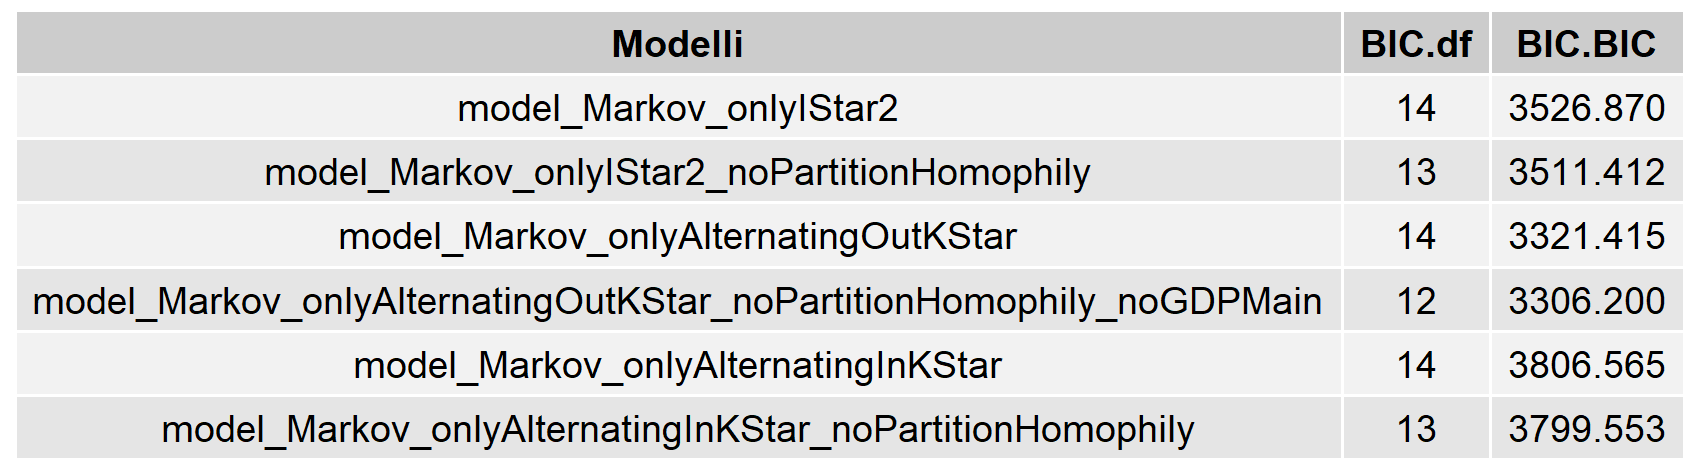
\includegraphics{images/markovModels_BIC.png}

    A quanto pare i modelli migliori risultano essere
`model\_Markov\_onlyAlternatingOutKStar' e
`model\_Markov\_onlyAlternatingOutKStar\_noPartitionHomophily\_noGDPMain',
adesso proviamo a simularli e verificare quale dei due modelli riesce a
catturare meglio le statistiche di rete e le statistiche nodali.

    \begin{tcolorbox}[breakable, size=fbox, boxrule=1pt, pad at break*=1mm,colback=cellbackground, colframe=cellborder]
\prompt{In}{incolor}{43}{\boxspacing}
\begin{Verbatim}[commandchars=\\\{\}]
\PY{n}{sim3}\PY{+w}{ }\PY{o}{\PYZlt{}\PYZhy{}}\PY{+w}{ }\PY{n+nf}{suppressMessages}\PY{p}{(}\PY{n+nf}{simulate}\PY{p}{(}\PY{n}{model\PYZus{}Markov\PYZus{}onlyAlternatingOutKStar}\PY{p}{,}\PY{+w}{ }\PY{n}{nsim}\PY{+w}{ }\PY{o}{=}\PY{+w}{ }\PY{l+m}{100}\PY{p}{,}\PY{+w}{ }\PY{n}{verbose}\PY{+w}{ }\PY{o}{=}\PY{+w}{ }\PY{k+kc}{TRUE}\PY{p}{,}\PY{+w}{ }\PY{n}{seed}\PY{+w}{ }\PY{o}{=}\PY{+w}{ }\PY{l+m}{1}\PY{p}{)}\PY{p}{)}

\PY{n}{null.distr3}\PY{+w}{ }\PY{o}{\PYZlt{}\PYZhy{}}\PY{+w}{ }\PY{n+nf}{matrix}\PY{p}{(}\PY{p}{,}\PY{l+m}{100}\PY{p}{,}\PY{l+m}{4}\PY{p}{)}
\PY{n+nf}{for}\PY{p}{(}\PY{n}{b}\PY{+w}{ }\PY{n}{in}\PY{+w}{ }\PY{l+m}{1}\PY{o}{:}\PY{l+m}{100}\PY{p}{)}\PY{p}{\PYZob{}}
\PY{+w}{	}\PY{n}{null.distr3}\PY{p}{[}\PY{n}{b}\PY{p}{,}\PY{p}{]}\PY{+w}{ }\PY{o}{\PYZlt{}\PYZhy{}}\PY{+w}{ }\PY{n+nf}{extractInformationsFromGraph}\PY{p}{(}\PY{n}{sim3}\PY{p}{[[}\PY{n}{b}\PY{p}{]]}\PY{p}{)}
\PY{p}{\PYZcb{}}

\PY{n}{sim4}\PY{+w}{ }\PY{o}{\PYZlt{}\PYZhy{}}\PY{+w}{ }\PY{n+nf}{suppressMessages}\PY{p}{(}\PY{p}{(}\PY{n+nf}{simulate}\PY{p}{(}\PY{n}{model\PYZus{}Markov\PYZus{}onlyAlternatingOutKStar\PYZus{}noPartitionHomophily\PYZus{}noGDPMain}\PY{p}{,}\PY{+w}{ }\PY{n}{nsim}\PY{+w}{ }\PY{o}{=}\PY{+w}{ }\PY{l+m}{100}\PY{p}{,}\PY{+w}{ }\PY{n}{verbose}\PY{+w}{ }\PY{o}{=}\PY{+w}{ }\PY{k+kc}{TRUE}\PY{p}{,}\PY{+w}{ }\PY{n}{seed}\PY{+w}{ }\PY{o}{=}\PY{+w}{ }\PY{l+m}{1}\PY{p}{)}\PY{p}{)}\PY{p}{)}

\PY{n}{null.distr4}\PY{+w}{ }\PY{o}{\PYZlt{}\PYZhy{}}\PY{+w}{ }\PY{n+nf}{matrix}\PY{p}{(}\PY{p}{,}\PY{l+m}{100}\PY{p}{,}\PY{l+m}{4}\PY{p}{)}
\PY{n+nf}{for}\PY{p}{(}\PY{n}{b}\PY{+w}{ }\PY{n}{in}\PY{+w}{ }\PY{l+m}{1}\PY{o}{:}\PY{l+m}{100}\PY{p}{)}\PY{p}{\PYZob{}}
\PY{+w}{	}\PY{n}{null.distr4}\PY{p}{[}\PY{n}{b}\PY{p}{,}\PY{p}{]}\PY{+w}{ }\PY{o}{\PYZlt{}\PYZhy{}}\PY{+w}{ }\PY{n+nf}{extractInformationsFromGraph}\PY{p}{(}\PY{n}{sim4}\PY{p}{[[}\PY{n}{b}\PY{p}{]]}\PY{p}{)}
\PY{p}{\PYZcb{}}
\end{Verbatim}
\end{tcolorbox}

    \begin{tcolorbox}[breakable, size=fbox, boxrule=1pt, pad at break*=1mm,colback=cellbackground, colframe=cellborder]
\prompt{In}{incolor}{44}{\boxspacing}
\begin{Verbatim}[commandchars=\\\{\}]
\PY{n+nf}{png}\PY{p}{(}\PY{l+s}{\PYZdq{}}\PY{l+s}{images/model\PYZus{}Markov\PYZus{}onlyAlternatingOutKStar\PYZus{}VS\PYZus{}model\PYZus{}Markov\PYZus{}onlyAlternatingOutKStar\PYZus{}noPartitionHomophily\PYZus{}noGDPMain\PYZus{}\PYZus{}Part1.png\PYZdq{}}\PY{p}{,}\PY{+w}{ }\PY{n}{width}\PY{+w}{ }\PY{o}{=}\PY{+w}{ }\PY{l+m}{1000}\PY{p}{,}\PY{+w}{ }\PY{n}{height}\PY{+w}{ }\PY{o}{=}\PY{+w}{ }\PY{l+m}{1000}\PY{p}{,}\PY{+w}{ }\PY{n}{res}\PY{+w}{ }\PY{o}{=}\PY{+w}{ }\PY{l+m}{150}\PY{p}{)}
\PY{n+nf}{par}\PY{p}{(}\PY{n}{mfrow}\PY{+w}{ }\PY{o}{=}\PY{+w}{ }\PY{n+nf}{c}\PY{p}{(}\PY{l+m}{4}\PY{p}{,}\PY{l+m}{1}\PY{p}{)}\PY{p}{)}
\PY{n+nf}{hist}\PY{p}{(}\PY{n+nf}{unlist}\PY{p}{(}\PY{n}{null.distr3}\PY{p}{[}\PY{p}{,}\PY{l+m}{2}\PY{p}{]}\PY{p}{)}\PY{p}{,}\PY{+w}{ }\PY{n}{xlab}\PY{+w}{ }\PY{o}{=}\PY{+w}{ }\PY{l+s}{\PYZdq{}}\PY{l+s}{in\PYZhy{}degree\PYZdq{}}\PY{p}{,}\PY{+w}{ }\PY{n}{xlim}\PY{+w}{ }\PY{o}{=}\PY{+w}{ }\PY{n+nf}{c}\PY{p}{(}\PY{l+m}{2}\PY{p}{,}\PY{l+m}{10}\PY{p}{)}\PY{p}{,}\PY{+w}{ }\PY{n}{main}\PY{+w}{ }\PY{o}{=}\PY{+w}{ }\PY{l+s}{\PYZdq{}}\PY{l+s}{In Degree Distribution with GDP Main and Partition Homophily\PYZdq{}}\PY{p}{)}\PY{p}{;}\PY{+w}{ }\PY{n+nf}{abline}\PY{p}{(}\PY{n}{v}\PY{+w}{ }\PY{o}{=}\PY{+w}{ }\PY{n+nf}{sd}\PY{p}{(}\PY{n+nf}{degree}\PY{p}{(}\PY{n}{g}\PY{p}{,}\PY{+w}{ }\PY{n}{mode}\PY{+w}{ }\PY{o}{=}\PY{+w}{ }\PY{l+s}{\PYZdq{}}\PY{l+s}{in\PYZdq{}}\PY{p}{)}\PY{p}{)}\PY{p}{,}\PY{+w}{ }\PY{n}{col}\PY{+w}{ }\PY{o}{=}\PY{+w}{ }\PY{l+s}{\PYZdq{}}\PY{l+s}{red\PYZdq{}}\PY{p}{)}
\PY{n+nf}{hist}\PY{p}{(}\PY{n+nf}{unlist}\PY{p}{(}\PY{n}{null.distr4}\PY{p}{[}\PY{p}{,}\PY{l+m}{2}\PY{p}{]}\PY{p}{)}\PY{p}{,}\PY{+w}{ }\PY{n}{xlab}\PY{+w}{ }\PY{o}{=}\PY{+w}{ }\PY{l+s}{\PYZdq{}}\PY{l+s}{in\PYZhy{}degree\PYZdq{}}\PY{p}{,}\PY{+w}{ }\PY{n}{xlim}\PY{+w}{ }\PY{o}{=}\PY{+w}{ }\PY{n+nf}{c}\PY{p}{(}\PY{l+m}{2}\PY{p}{,}\PY{l+m}{10}\PY{p}{)}\PY{p}{,}\PY{+w}{ }\PY{n}{main}\PY{+w}{ }\PY{o}{=}\PY{+w}{ }\PY{l+s}{\PYZdq{}}\PY{l+s}{In Degree Distribution without GDP Main and Partition Homophily\PYZdq{}}\PY{p}{)}\PY{p}{;}\PY{+w}{ }\PY{n+nf}{abline}\PY{p}{(}\PY{n}{v}\PY{+w}{ }\PY{o}{=}\PY{+w}{ }\PY{n+nf}{sd}\PY{p}{(}\PY{n+nf}{degree}\PY{p}{(}\PY{n}{g}\PY{p}{,}\PY{+w}{ }\PY{n}{mode}\PY{+w}{ }\PY{o}{=}\PY{+w}{ }\PY{l+s}{\PYZdq{}}\PY{l+s}{in\PYZdq{}}\PY{p}{)}\PY{p}{)}\PY{p}{,}\PY{+w}{ }\PY{n}{col}\PY{+w}{ }\PY{o}{=}\PY{+w}{ }\PY{l+s}{\PYZdq{}}\PY{l+s}{red\PYZdq{}}\PY{p}{)}
\PY{n+nf}{hist}\PY{p}{(}\PY{n+nf}{unlist}\PY{p}{(}\PY{n}{null.distr3}\PY{p}{[}\PY{p}{,}\PY{l+m}{3}\PY{p}{]}\PY{p}{)}\PY{p}{,}\PY{+w}{ }\PY{n}{xlab}\PY{+w}{ }\PY{o}{=}\PY{+w}{ }\PY{l+s}{\PYZdq{}}\PY{l+s}{out\PYZhy{}degree\PYZdq{}}\PY{p}{,}\PY{+w}{ }\PY{n}{xlim}\PY{+w}{ }\PY{o}{=}\PY{+w}{ }\PY{n+nf}{c}\PY{p}{(}\PY{l+m}{12}\PY{p}{,}\PY{+w}{ }\PY{l+m}{20}\PY{p}{)}\PY{p}{,}\PY{+w}{ }\PY{n}{main}\PY{+w}{ }\PY{o}{=}\PY{+w}{ }\PY{l+s}{\PYZdq{}}\PY{l+s}{Out Degree Distribution with GDP Main and Partition Homophily\PYZdq{}}\PY{p}{)}\PY{p}{;}\PY{+w}{ }\PY{n+nf}{abline}\PY{p}{(}\PY{n}{v}\PY{+w}{ }\PY{o}{=}\PY{+w}{ }\PY{n+nf}{sd}\PY{p}{(}\PY{n+nf}{degree}\PY{p}{(}\PY{n}{g}\PY{p}{,}\PY{+w}{ }\PY{n}{mode}\PY{+w}{ }\PY{o}{=}\PY{+w}{ }\PY{l+s}{\PYZdq{}}\PY{l+s}{out\PYZdq{}}\PY{p}{)}\PY{p}{)}\PY{p}{,}\PY{+w}{ }\PY{n}{col}\PY{+w}{ }\PY{o}{=}\PY{+w}{ }\PY{l+s}{\PYZdq{}}\PY{l+s}{red\PYZdq{}}\PY{p}{)}
\PY{n+nf}{hist}\PY{p}{(}\PY{n+nf}{unlist}\PY{p}{(}\PY{n}{null.distr4}\PY{p}{[}\PY{p}{,}\PY{l+m}{3}\PY{p}{]}\PY{p}{)}\PY{p}{,}\PY{+w}{ }\PY{n}{xlab}\PY{+w}{ }\PY{o}{=}\PY{+w}{ }\PY{l+s}{\PYZdq{}}\PY{l+s}{out\PYZhy{}degree\PYZdq{}}\PY{p}{,}\PY{+w}{ }\PY{n}{xlim}\PY{+w}{ }\PY{o}{=}\PY{+w}{ }\PY{n+nf}{c}\PY{p}{(}\PY{l+m}{12}\PY{p}{,}\PY{+w}{ }\PY{l+m}{20}\PY{p}{)}\PY{p}{,}\PY{+w}{ }\PY{n}{main}\PY{+w}{ }\PY{o}{=}\PY{+w}{ }\PY{l+s}{\PYZdq{}}\PY{l+s}{Out Degree Distribution without GDP Main and Partition Homophily\PYZdq{}}\PY{p}{)}\PY{p}{;}\PY{+w}{ }\PY{n+nf}{abline}\PY{p}{(}\PY{n}{v}\PY{+w}{ }\PY{o}{=}\PY{+w}{ }\PY{n+nf}{sd}\PY{p}{(}\PY{n+nf}{degree}\PY{p}{(}\PY{n}{g}\PY{p}{,}\PY{+w}{ }\PY{n}{mode}\PY{+w}{ }\PY{o}{=}\PY{+w}{ }\PY{l+s}{\PYZdq{}}\PY{l+s}{out\PYZdq{}}\PY{p}{)}\PY{p}{)}\PY{p}{,}\PY{+w}{ }\PY{n}{col}\PY{+w}{ }\PY{o}{=}\PY{+w}{ }\PY{l+s}{\PYZdq{}}\PY{l+s}{red\PYZdq{}}\PY{p}{)}
\PY{n+nf}{invisible}\PY{p}{(}\PY{n+nf}{dev.off}\PY{p}{(}\PY{p}{)}\PY{p}{)}

\PY{n+nf}{png}\PY{p}{(}\PY{l+s}{\PYZdq{}}\PY{l+s}{images/model\PYZus{}Markov\PYZus{}onlyAlternatingOutKStar\PYZus{}VS\PYZus{}model\PYZus{}Markov\PYZus{}onlyAlternatingOutKStar\PYZus{}noPartitionHomophily\PYZus{}noGDPMain\PYZus{}\PYZus{}Part2.png\PYZdq{}}\PY{p}{,}\PY{+w}{ }\PY{n}{width}\PY{+w}{ }\PY{o}{=}\PY{+w}{ }\PY{l+m}{1000}\PY{p}{,}\PY{+w}{ }\PY{n}{height}\PY{+w}{ }\PY{o}{=}\PY{+w}{ }\PY{l+m}{1000}\PY{p}{,}\PY{+w}{ }\PY{n}{res}\PY{+w}{ }\PY{o}{=}\PY{+w}{ }\PY{l+m}{150}\PY{p}{)}
\PY{n+nf}{par}\PY{p}{(}\PY{n}{mfrow}\PY{+w}{ }\PY{o}{=}\PY{+w}{ }\PY{n+nf}{c}\PY{p}{(}\PY{l+m}{4}\PY{p}{,}\PY{l+m}{1}\PY{p}{)}\PY{p}{)}
\PY{n+nf}{hist}\PY{p}{(}\PY{n+nf}{unlist}\PY{p}{(}\PY{n}{null.distr3}\PY{p}{[}\PY{p}{,}\PY{l+m}{1}\PY{p}{]}\PY{p}{)}\PY{p}{,}\PY{+w}{ }\PY{n}{xlab}\PY{+w}{ }\PY{o}{=}\PY{+w}{ }\PY{l+s}{\PYZdq{}}\PY{l+s}{transitivity\PYZdq{}}\PY{p}{,}\PY{+w}{ }\PY{n}{xlim}\PY{+w}{ }\PY{o}{=}\PY{+w}{ }\PY{n+nf}{c}\PY{p}{(}\PY{l+m}{0.40}\PY{p}{,}\PY{+w}{ }\PY{l+m}{0.48}\PY{p}{)}\PY{p}{,}\PY{+w}{ }\PY{n}{main}\PY{+w}{ }\PY{o}{=}\PY{+w}{ }\PY{l+s}{\PYZdq{}}\PY{l+s}{Transitivity Distribution with GDP Main and Partition Homophily\PYZdq{}}\PY{p}{)}\PY{p}{;}\PY{+w}{ }\PY{n+nf}{abline}\PY{p}{(}\PY{n}{v}\PY{+w}{ }\PY{o}{=}\PY{+w}{ }\PY{n+nf}{transitivity}\PY{p}{(}\PY{n}{g}\PY{p}{)}\PY{p}{,}\PY{+w}{ }\PY{n}{col}\PY{+w}{ }\PY{o}{=}\PY{+w}{ }\PY{l+s}{\PYZdq{}}\PY{l+s}{red\PYZdq{}}\PY{p}{)}
\PY{n+nf}{hist}\PY{p}{(}\PY{n+nf}{unlist}\PY{p}{(}\PY{n}{null.distr4}\PY{p}{[}\PY{p}{,}\PY{l+m}{1}\PY{p}{]}\PY{p}{)}\PY{p}{,}\PY{+w}{ }\PY{n}{xlab}\PY{+w}{ }\PY{o}{=}\PY{+w}{ }\PY{l+s}{\PYZdq{}}\PY{l+s}{transitivity\PYZdq{}}\PY{p}{,}\PY{+w}{ }\PY{n}{xlim}\PY{+w}{ }\PY{o}{=}\PY{+w}{ }\PY{n+nf}{c}\PY{p}{(}\PY{l+m}{0.40}\PY{p}{,}\PY{+w}{ }\PY{l+m}{0.48}\PY{p}{)}\PY{p}{,}\PY{+w}{ }\PY{n}{main}\PY{+w}{ }\PY{o}{=}\PY{+w}{ }\PY{l+s}{\PYZdq{}}\PY{l+s}{Transitivity Distribution without GDP Main and Partition Homophily\PYZdq{}}\PY{p}{)}\PY{p}{;}\PY{+w}{ }\PY{n+nf}{abline}\PY{p}{(}\PY{n}{v}\PY{+w}{ }\PY{o}{=}\PY{+w}{ }\PY{n+nf}{transitivity}\PY{p}{(}\PY{n}{g}\PY{p}{)}\PY{p}{,}\PY{+w}{ }\PY{n}{col}\PY{+w}{ }\PY{o}{=}\PY{+w}{ }\PY{l+s}{\PYZdq{}}\PY{l+s}{red\PYZdq{}}\PY{p}{)}
\PY{n+nf}{hist}\PY{p}{(}\PY{n+nf}{unlist}\PY{p}{(}\PY{n}{null.distr3}\PY{p}{[}\PY{p}{,}\PY{l+m}{4}\PY{p}{]}\PY{p}{)}\PY{p}{,}\PY{+w}{ }\PY{n}{xlab}\PY{+w}{ }\PY{o}{=}\PY{+w}{ }\PY{l+s}{\PYZdq{}}\PY{l+s}{density\PYZdq{}}\PY{p}{,}\PY{+w}{ }\PY{n}{xlim}\PY{+w}{ }\PY{o}{=}\PY{+w}{ }\PY{n+nf}{c}\PY{p}{(}\PY{l+m}{0.13}\PY{p}{,}\PY{+w}{ }\PY{l+m}{0.19}\PY{p}{)}\PY{p}{,}\PY{+w}{ }\PY{n}{main}\PY{+w}{ }\PY{o}{=}\PY{+w}{ }\PY{l+s}{\PYZdq{}}\PY{l+s}{Density Distribution with GDP Main and Partition Homophily\PYZdq{}}\PY{p}{)}\PY{p}{;}\PY{+w}{ }\PY{n+nf}{abline}\PY{p}{(}\PY{n}{v}\PY{+w}{ }\PY{o}{=}\PY{+w}{ }\PY{n+nf}{edge\PYZus{}density}\PY{p}{(}\PY{n}{g}\PY{p}{)}\PY{p}{,}\PY{+w}{ }\PY{n}{col}\PY{+w}{ }\PY{o}{=}\PY{+w}{ }\PY{l+s}{\PYZdq{}}\PY{l+s}{red\PYZdq{}}\PY{p}{)}
\PY{n+nf}{hist}\PY{p}{(}\PY{n+nf}{unlist}\PY{p}{(}\PY{n}{null.distr4}\PY{p}{[}\PY{p}{,}\PY{l+m}{4}\PY{p}{]}\PY{p}{)}\PY{p}{,}\PY{+w}{ }\PY{n}{xlab}\PY{+w}{ }\PY{o}{=}\PY{+w}{ }\PY{l+s}{\PYZdq{}}\PY{l+s}{density\PYZdq{}}\PY{p}{,}\PY{+w}{ }\PY{n}{xlim}\PY{+w}{ }\PY{o}{=}\PY{+w}{ }\PY{n+nf}{c}\PY{p}{(}\PY{l+m}{0.13}\PY{p}{,}\PY{+w}{ }\PY{l+m}{0.19}\PY{p}{)}\PY{p}{,}\PY{+w}{ }\PY{n}{main}\PY{+w}{ }\PY{o}{=}\PY{+w}{ }\PY{l+s}{\PYZdq{}}\PY{l+s}{Density Distribution without GDP Main and Partition Homophily\PYZdq{}}\PY{p}{)}\PY{p}{;}\PY{+w}{ }\PY{n+nf}{abline}\PY{p}{(}\PY{n}{v}\PY{+w}{ }\PY{o}{=}\PY{+w}{ }\PY{n+nf}{edge\PYZus{}density}\PY{p}{(}\PY{n}{g}\PY{p}{)}\PY{p}{,}\PY{+w}{ }\PY{n}{col}\PY{+w}{ }\PY{o}{=}\PY{+w}{ }\PY{l+s}{\PYZdq{}}\PY{l+s}{red\PYZdq{}}\PY{p}{)}
\PY{n+nf}{invisible}\PY{p}{(}\PY{n+nf}{dev.off}\PY{p}{(}\PY{p}{)}\PY{p}{)}
\end{Verbatim}
\end{tcolorbox}

    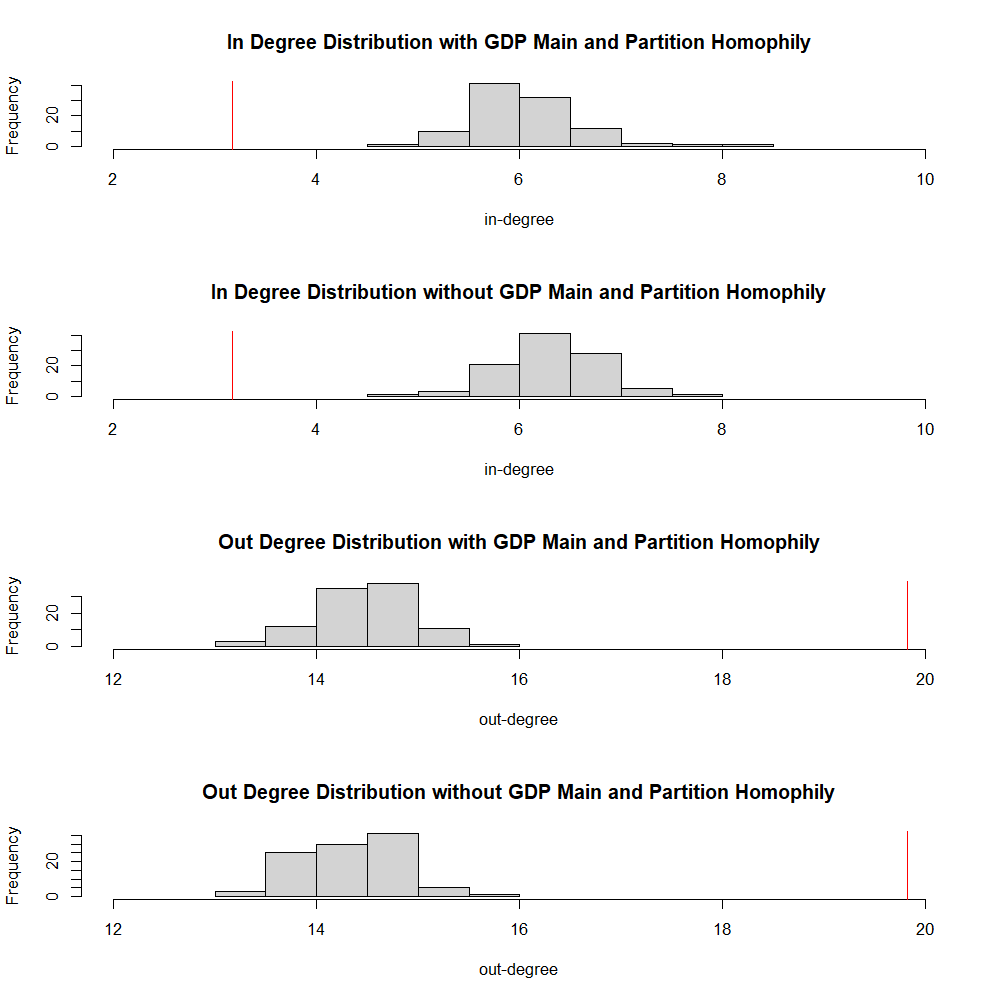
\includegraphics{images/model_Markov_onlyAlternatingOutKStar_VS_model_Markov_onlyAlternatingOutKStar_noPartitionHomophily_noGDPMain__Part1.png}

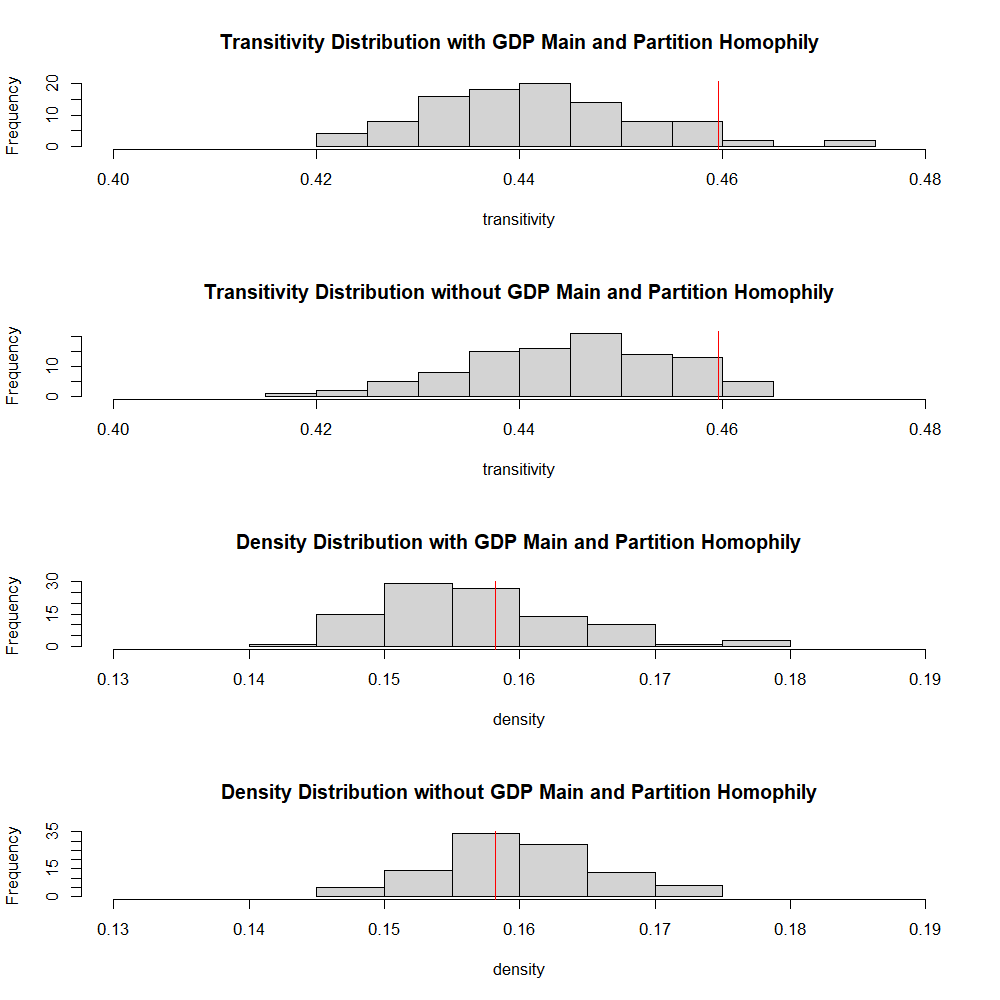
\includegraphics{images/model_Markov_onlyAlternatingOutKStar_VS_model_Markov_onlyAlternatingOutKStar_noPartitionHomophily_noGDPMain__Part2.png}

    I due modelli si comportano in modo molto simile. Il modello che
scegliamo è il secondo (per via della minore complessità).

    \subsubsection{Social Circuit Model}\label{social-circuit-model}

Infine abbiamo provato a generare dei modelli basati sulle condizioni
del Social Circuit, ma sfortunatamente alcuni di essi hanno dato
Degeneracy Problems. Siamo stati in grado di generare soltanto un
modello basato sulle K-2 Paths.

    \begin{tcolorbox}[breakable, size=fbox, boxrule=1pt, pad at break*=1mm,colback=cellbackground, colframe=cellborder]
\prompt{In}{incolor}{45}{\boxspacing}
\begin{Verbatim}[commandchars=\\\{\}]
\PY{n+nf}{summary}\PY{p}{(}\PY{n}{model\PYZus{}SocialCirtcuit\PYZus{}onlyK2Paths}\PY{p}{)}
\end{Verbatim}
\end{tcolorbox}

    
    \begin{Verbatim}[commandchars=\\\{\}]
Call:
ergm(formula = net \textasciitilde{} edges + mutual + nodecov("gdp") + nodefactor("continent") + 
    nodefactor("partition") + absdiff("gdp") + nodematch("continent") + 
    nodematch("partition") + gwdsp(decay = 1, fixed = T), control = control.ergm(seed = 1), 
    verbose = 2)

Monte Carlo Maximum Likelihood Results:

                         Estimate Std. Error MCMC \% z value Pr(>|z|)    
edges                   3.841e+00  3.459e-01      0  11.104   <1e-04 ***
mutual                 -1.302e-01  1.851e-01      0  -0.704   0.4816    
nodecov.gdp             3.804e-06  3.636e-06      0   1.046   0.2954    
nodefactor.continent.2  3.563e-02  1.217e-01      0   0.293   0.7696    
nodefactor.continent.3 -7.404e-01  1.274e-01      0  -5.812   <1e-04 ***
nodefactor.continent.4  1.028e+00  1.572e-01      0   6.540   <1e-04 ***
nodefactor.continent.5  7.795e-01  1.803e-01      0   4.323   <1e-04 ***
nodefactor.continent.6  2.247e-02  1.263e-01      0   0.178   0.8588    
nodefactor.partition.2 -2.547e+00  1.621e-01      0 -15.709   <1e-04 ***
nodefactor.partition.3 -4.068e+00  1.931e-01      0 -21.069   <1e-04 ***
absdiff.gdp            -9.804e-06  4.931e-06      0  -1.988   0.0468 *  
nodematch.continent     2.243e+00  1.192e-01      0  18.813   <1e-04 ***
nodematch.partition    -8.017e-01  1.467e-01      0  -5.466   <1e-04 ***
gwdsp.OTP.fixed.1      -1.272e-01  5.888e-03      0 -21.605   <1e-04 ***
---
Signif. codes:  0 '***' 0.001 '**' 0.01 '*' 0.05 '.' 0.1 ' ' 1

     Null Deviance: 8761  on 6320  degrees of freedom
 Residual Deviance: 2985  on 6306  degrees of freedom
 
AIC: 3013  BIC: 3108  (Smaller is better. MC Std. Err. = 1.056)
    \end{Verbatim}

    
    Dal summary si può notare che l'effetto di reciprocità e l'effetto
principale del GDP non vengono considerati come significativi, quindi
proviamo a calcolare un modello togliendo tali effetti.

    \begin{tcolorbox}[breakable, size=fbox, boxrule=1pt, pad at break*=1mm,colback=cellbackground, colframe=cellborder]
\prompt{In}{incolor}{46}{\boxspacing}
\begin{Verbatim}[commandchars=\\\{\}]
\PY{n+nf}{summary}\PY{p}{(}\PY{n}{model\PYZus{}SocialCirtcuit\PYZus{}onlyK2Paths\PYZus{}NoMutualEffect\PYZus{}NoGDPMain}\PY{p}{)}
\end{Verbatim}
\end{tcolorbox}

    
    \begin{Verbatim}[commandchars=\\\{\}]
Call:
ergm(formula = net \textasciitilde{} edges + nodefactor("continent") + nodefactor("partition") + 
    absdiff("gdp") + nodematch("continent") + nodematch("partition") + 
    gwdsp(decay = 1, fixed = T), control = control.ergm(seed = 1, 
    checkpoint = "mod5\_gwdsp\_2/step\_\%03d.RData"), verbose = 2)

Monte Carlo Maximum Likelihood Results:

                         Estimate Std. Error MCMC \% z value Pr(>|z|)    
edges                   3.932e+00  3.055e-01      0  12.870   <1e-04 ***
nodefactor.continent.2  4.571e-02  1.167e-01      0   0.392   0.6952    
nodefactor.continent.3 -7.139e-01  1.235e-01      0  -5.780   <1e-04 ***
nodefactor.continent.4  1.028e+00  1.531e-01      0   6.716   <1e-04 ***
nodefactor.continent.5  7.981e-01  1.705e-01      0   4.680   <1e-04 ***
nodefactor.continent.6  3.193e-02  1.255e-01      0   0.254   0.7992    
nodefactor.partition.2 -2.567e+00  1.452e-01      0 -17.682   <1e-04 ***
nodefactor.partition.3 -4.086e+00  1.570e-01      0 -26.028   <1e-04 ***
absdiff.gdp            -9.242e-06  4.867e-06      0  -1.899   0.0576 .  
nodematch.continent     2.210e+00  1.074e-01      0  20.574   <1e-04 ***
nodematch.partition    -8.075e-01  1.460e-01      0  -5.530   <1e-04 ***
gwdsp.OTP.fixed.1      -1.298e-01  4.480e-03      0 -28.968   <1e-04 ***
---
Signif. codes:  0 '***' 0.001 '**' 0.01 '*' 0.05 '.' 0.1 ' ' 1

     Null Deviance: 8761  on 6320  degrees of freedom
 Residual Deviance: 2988  on 6308  degrees of freedom
 
AIC: 3012  BIC: 3093  (Smaller is better. MC Std. Err. = 0.8983)
    \end{Verbatim}

    
    Adesso andiamo a confrontare i modelli appena calcolati con il
precedente migliore modello (cioè
`model\_Markov\_onlyAlternatingOutKStar\_noPartitionHomophily\_noGDPMain')

    \begin{tcolorbox}[breakable, size=fbox, boxrule=1pt, pad at break*=1mm,colback=cellbackground, colframe=cellborder]
\prompt{In}{incolor}{47}{\boxspacing}
\begin{Verbatim}[commandchars=\\\{\}]
\PY{n}{table}\PY{+w}{ }\PY{o}{\PYZlt{}\PYZhy{}}\PY{+w}{ }\PY{n+nf}{data.frame}\PY{p}{(}
\PY{+w}{    }\PY{n}{Modelli}\PY{+w}{ }\PY{o}{=}\PY{+w}{ }\PY{n+nf}{c}\PY{p}{(}\PY{l+s}{\PYZdq{}}\PY{l+s}{model\PYZus{}Markov\PYZus{}onlyAlternatingOutKStar\PYZus{}noPartitionHomophily\PYZus{}noGDPMain\PYZdq{}}\PY{p}{,}\PY{+w}{ }\PY{l+s}{\PYZdq{}}\PY{l+s}{model\PYZus{}SocialCirtcuit\PYZus{}onlyK2Paths\PYZdq{}}\PY{p}{,}\PY{+w}{ }\PY{l+s}{\PYZdq{}}\PY{l+s}{model\PYZus{}SocialCirtcuit\PYZus{}onlyK2Paths\PYZus{}NoMutualEffect\PYZus{}NoGDPMain\PYZdq{}}\PY{p}{)}\PY{p}{,}
\PY{+w}{    }\PY{n}{BIC}\PY{+w}{ }\PY{o}{=}\PY{+w}{ }\PY{n+nf}{BIC}\PY{p}{(}\PY{n}{model\PYZus{}Markov\PYZus{}onlyAlternatingOutKStar\PYZus{}noPartitionHomophily\PYZus{}noGDPMain}\PY{p}{,}\PY{+w}{ }\PY{n}{model\PYZus{}SocialCirtcuit\PYZus{}onlyK2Paths}\PY{p}{,}\PY{+w}{ }\PY{n}{model\PYZus{}SocialCirtcuit\PYZus{}onlyK2Paths\PYZus{}NoMutualEffect\PYZus{}NoGDPMain}\PY{p}{)}
\PY{p}{)}
\PY{n+nf}{createImageFromTable}\PY{p}{(}\PY{n}{table}\PY{p}{,}\PY{+w}{ }\PY{l+s}{\PYZdq{}}\PY{l+s}{images/socialCircuitModels\PYZus{}BIC.png\PYZdq{}}\PY{p}{,}\PY{+w}{ }\PY{l+m}{1700}\PY{p}{,}\PY{+w}{ }\PY{l+m}{300}\PY{p}{,}\PY{+w}{ }\PY{l+m}{230}\PY{p}{)}
\end{Verbatim}
\end{tcolorbox}

    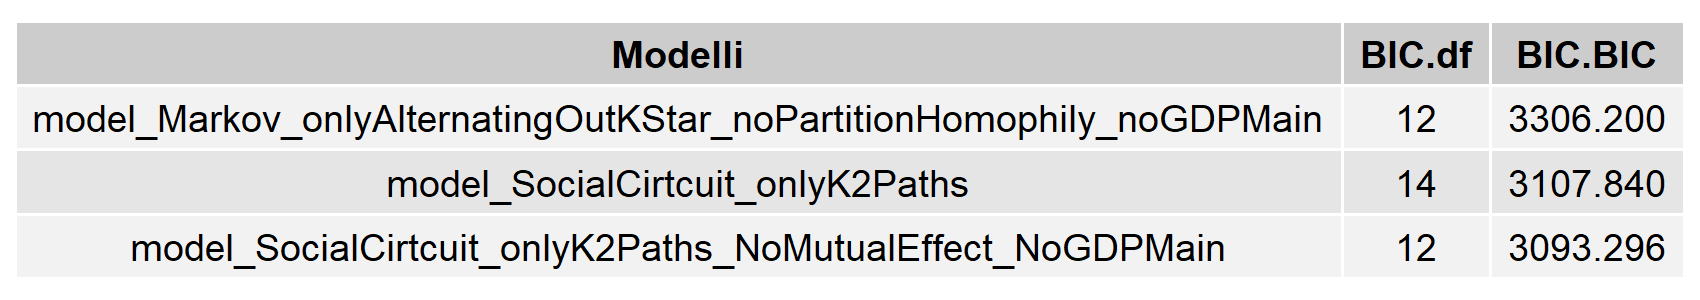
\includegraphics{images/socialCircuitModels_BIC.png}

    I due nuovi modelli sono entrambi migliori del precedente e hanno
punteggi molto simili, quindi andiamo a verificare quale dei due riesce
a catturare meglio le statistiche di rete e le statistiche nodali

    \begin{tcolorbox}[breakable, size=fbox, boxrule=1pt, pad at break*=1mm,colback=cellbackground, colframe=cellborder]
\prompt{In}{incolor}{48}{\boxspacing}
\begin{Verbatim}[commandchars=\\\{\}]
\PY{n}{sim5}\PY{+w}{ }\PY{o}{\PYZlt{}\PYZhy{}}\PY{+w}{ }\PY{n+nf}{suppressMessages}\PY{p}{(}\PY{n+nf}{simulate}\PY{p}{(}\PY{n}{model\PYZus{}SocialCirtcuit\PYZus{}onlyK2Paths}\PY{p}{,}\PY{+w}{ }\PY{n}{nsim}\PY{+w}{ }\PY{o}{=}\PY{+w}{ }\PY{l+m}{100}\PY{p}{,}\PY{+w}{ }\PY{n}{verbose}\PY{+w}{ }\PY{o}{=}\PY{+w}{ }\PY{k+kc}{TRUE}\PY{p}{,}\PY{+w}{ }\PY{n}{seed}\PY{+w}{ }\PY{o}{=}\PY{+w}{ }\PY{l+m}{1}\PY{p}{)}\PY{p}{)}

\PY{n}{null.distr5}\PY{+w}{ }\PY{o}{\PYZlt{}\PYZhy{}}\PY{+w}{ }\PY{n+nf}{matrix}\PY{p}{(}\PY{p}{,}\PY{l+m}{100}\PY{p}{,}\PY{l+m}{4}\PY{p}{)}
\PY{n+nf}{for}\PY{p}{(}\PY{n}{b}\PY{+w}{ }\PY{n}{in}\PY{+w}{ }\PY{l+m}{1}\PY{o}{:}\PY{l+m}{100}\PY{p}{)}\PY{p}{\PYZob{}}
\PY{+w}{	}\PY{n}{null.distr5}\PY{p}{[}\PY{n}{b}\PY{p}{,}\PY{p}{]}\PY{+w}{ }\PY{o}{\PYZlt{}\PYZhy{}}\PY{+w}{ }\PY{n+nf}{extractInformationsFromGraph}\PY{p}{(}\PY{n}{sim5}\PY{p}{[[}\PY{n}{b}\PY{p}{]]}\PY{p}{)}
\PY{p}{\PYZcb{}}

\PY{n}{sim6}\PY{+w}{ }\PY{o}{\PYZlt{}\PYZhy{}}\PY{+w}{ }\PY{n+nf}{suppressMessages}\PY{p}{(}\PY{p}{(}\PY{n+nf}{simulate}\PY{p}{(}\PY{n}{model\PYZus{}SocialCirtcuit\PYZus{}onlyK2Paths\PYZus{}NoMutualEffect\PYZus{}NoGDPMain}\PY{p}{,}\PY{+w}{ }\PY{n}{nsim}\PY{+w}{ }\PY{o}{=}\PY{+w}{ }\PY{l+m}{100}\PY{p}{,}\PY{+w}{ }\PY{n}{verbose}\PY{+w}{ }\PY{o}{=}\PY{+w}{ }\PY{k+kc}{TRUE}\PY{p}{,}\PY{+w}{ }\PY{n}{seed}\PY{+w}{ }\PY{o}{=}\PY{+w}{ }\PY{l+m}{1}\PY{p}{)}\PY{p}{)}\PY{p}{)}

\PY{n}{null.distr6}\PY{+w}{ }\PY{o}{\PYZlt{}\PYZhy{}}\PY{+w}{ }\PY{n+nf}{matrix}\PY{p}{(}\PY{p}{,}\PY{l+m}{100}\PY{p}{,}\PY{l+m}{4}\PY{p}{)}
\PY{n+nf}{for}\PY{p}{(}\PY{n}{b}\PY{+w}{ }\PY{n}{in}\PY{+w}{ }\PY{l+m}{1}\PY{o}{:}\PY{l+m}{100}\PY{p}{)}\PY{p}{\PYZob{}}
\PY{+w}{	}\PY{n}{null.distr6}\PY{p}{[}\PY{n}{b}\PY{p}{,}\PY{p}{]}\PY{+w}{ }\PY{o}{\PYZlt{}\PYZhy{}}\PY{+w}{ }\PY{n+nf}{extractInformationsFromGraph}\PY{p}{(}\PY{n}{sim6}\PY{p}{[[}\PY{n}{b}\PY{p}{]]}\PY{p}{)}
\PY{p}{\PYZcb{}}
\end{Verbatim}
\end{tcolorbox}

    \begin{tcolorbox}[breakable, size=fbox, boxrule=1pt, pad at break*=1mm,colback=cellbackground, colframe=cellborder]
\prompt{In}{incolor}{49}{\boxspacing}
\begin{Verbatim}[commandchars=\\\{\}]
\PY{n+nf}{png}\PY{p}{(}\PY{l+s}{\PYZdq{}}\PY{l+s}{images/model\PYZus{}SocialCirtcuit\PYZus{}onlyK2Paths\PYZus{}VS\PYZus{}model\PYZus{}SocialCirtcuit\PYZus{}onlyK2Paths\PYZus{}NoMutualEffect\PYZus{}NoGDPMain\PYZus{}\PYZus{}Part1.png\PYZdq{}}\PY{p}{,}\PY{+w}{ }\PY{n}{width}\PY{+w}{ }\PY{o}{=}\PY{+w}{ }\PY{l+m}{1000}\PY{p}{,}\PY{+w}{ }\PY{n}{height}\PY{+w}{ }\PY{o}{=}\PY{+w}{ }\PY{l+m}{1000}\PY{p}{,}\PY{+w}{ }\PY{n}{res}\PY{+w}{ }\PY{o}{=}\PY{+w}{ }\PY{l+m}{150}\PY{p}{)}
\PY{n+nf}{par}\PY{p}{(}\PY{n}{mfrow}\PY{+w}{ }\PY{o}{=}\PY{+w}{ }\PY{n+nf}{c}\PY{p}{(}\PY{l+m}{4}\PY{p}{,}\PY{l+m}{1}\PY{p}{)}\PY{p}{)}
\PY{n+nf}{hist}\PY{p}{(}\PY{n+nf}{unlist}\PY{p}{(}\PY{n}{null.distr5}\PY{p}{[}\PY{p}{,}\PY{l+m}{2}\PY{p}{]}\PY{p}{)}\PY{p}{,}\PY{+w}{ }\PY{n}{xlab}\PY{+w}{ }\PY{o}{=}\PY{+w}{ }\PY{l+s}{\PYZdq{}}\PY{l+s}{in\PYZhy{}degree\PYZdq{}}\PY{p}{,}\PY{+w}{ }\PY{n}{xlim}\PY{+w}{ }\PY{o}{=}\PY{+w}{ }\PY{n+nf}{c}\PY{p}{(}\PY{l+m}{2}\PY{p}{,}\PY{l+m}{10}\PY{p}{)}\PY{p}{,}\PY{+w}{ }\PY{n}{main}\PY{+w}{ }\PY{o}{=}\PY{+w}{ }\PY{l+s}{\PYZdq{}}\PY{l+s}{In Degree Distribution with Mutual Effect and GDP Main\PYZdq{}}\PY{p}{)}\PY{p}{;}\PY{+w}{ }\PY{n+nf}{abline}\PY{p}{(}\PY{n}{v}\PY{+w}{ }\PY{o}{=}\PY{+w}{ }\PY{n+nf}{sd}\PY{p}{(}\PY{n+nf}{degree}\PY{p}{(}\PY{n}{g}\PY{p}{,}\PY{+w}{ }\PY{n}{mode}\PY{+w}{ }\PY{o}{=}\PY{+w}{ }\PY{l+s}{\PYZdq{}}\PY{l+s}{in\PYZdq{}}\PY{p}{)}\PY{p}{)}\PY{p}{,}\PY{+w}{ }\PY{n}{col}\PY{+w}{ }\PY{o}{=}\PY{+w}{ }\PY{l+s}{\PYZdq{}}\PY{l+s}{red\PYZdq{}}\PY{p}{)}
\PY{n+nf}{hist}\PY{p}{(}\PY{n+nf}{unlist}\PY{p}{(}\PY{n}{null.distr6}\PY{p}{[}\PY{p}{,}\PY{l+m}{2}\PY{p}{]}\PY{p}{)}\PY{p}{,}\PY{+w}{ }\PY{n}{xlab}\PY{+w}{ }\PY{o}{=}\PY{+w}{ }\PY{l+s}{\PYZdq{}}\PY{l+s}{in\PYZhy{}degree\PYZdq{}}\PY{p}{,}\PY{+w}{ }\PY{n}{xlim}\PY{+w}{ }\PY{o}{=}\PY{+w}{ }\PY{n+nf}{c}\PY{p}{(}\PY{l+m}{0}\PY{p}{,}\PY{l+m}{20}\PY{p}{)}\PY{p}{,}\PY{+w}{ }\PY{n}{main}\PY{+w}{ }\PY{o}{=}\PY{+w}{ }\PY{l+s}{\PYZdq{}}\PY{l+s}{In Degree Distribution without Mutual Effect and GDP Main\PYZdq{}}\PY{p}{)}\PY{p}{;}\PY{+w}{ }\PY{n+nf}{abline}\PY{p}{(}\PY{n}{v}\PY{+w}{ }\PY{o}{=}\PY{+w}{ }\PY{n+nf}{sd}\PY{p}{(}\PY{n+nf}{degree}\PY{p}{(}\PY{n}{g}\PY{p}{,}\PY{+w}{ }\PY{n}{mode}\PY{+w}{ }\PY{o}{=}\PY{+w}{ }\PY{l+s}{\PYZdq{}}\PY{l+s}{in\PYZdq{}}\PY{p}{)}\PY{p}{)}\PY{p}{,}\PY{+w}{ }\PY{n}{col}\PY{+w}{ }\PY{o}{=}\PY{+w}{ }\PY{l+s}{\PYZdq{}}\PY{l+s}{red\PYZdq{}}\PY{p}{)}
\PY{n+nf}{hist}\PY{p}{(}\PY{n+nf}{unlist}\PY{p}{(}\PY{n}{null.distr5}\PY{p}{[}\PY{p}{,}\PY{l+m}{3}\PY{p}{]}\PY{p}{)}\PY{p}{,}\PY{+w}{ }\PY{n}{xlab}\PY{+w}{ }\PY{o}{=}\PY{+w}{ }\PY{l+s}{\PYZdq{}}\PY{l+s}{out\PYZhy{}degree\PYZdq{}}\PY{p}{,}\PY{+w}{ }\PY{n}{xlim}\PY{o}{=}\PY{n+nf}{c}\PY{p}{(}\PY{l+m}{12}\PY{p}{,}\PY{+w}{ }\PY{l+m}{20}\PY{p}{)}\PY{p}{,}\PY{+w}{ }\PY{n}{main}\PY{+w}{ }\PY{o}{=}\PY{+w}{ }\PY{l+s}{\PYZdq{}}\PY{l+s}{Out Degree Distribution with Mutual Effect and GDP Main\PYZdq{}}\PY{p}{)}\PY{p}{;}\PY{+w}{ }\PY{n+nf}{abline}\PY{p}{(}\PY{n}{v}\PY{+w}{ }\PY{o}{=}\PY{+w}{ }\PY{n+nf}{sd}\PY{p}{(}\PY{n+nf}{degree}\PY{p}{(}\PY{n}{g}\PY{p}{,}\PY{+w}{ }\PY{n}{mode}\PY{+w}{ }\PY{o}{=}\PY{+w}{ }\PY{l+s}{\PYZdq{}}\PY{l+s}{out\PYZdq{}}\PY{p}{)}\PY{p}{)}\PY{p}{,}\PY{+w}{ }\PY{n}{col}\PY{+w}{ }\PY{o}{=}\PY{+w}{ }\PY{l+s}{\PYZdq{}}\PY{l+s}{red\PYZdq{}}\PY{p}{)}
\PY{n+nf}{hist}\PY{p}{(}\PY{n+nf}{unlist}\PY{p}{(}\PY{n}{null.distr6}\PY{p}{[}\PY{p}{,}\PY{l+m}{3}\PY{p}{]}\PY{p}{)}\PY{p}{,}\PY{+w}{ }\PY{n}{xlab}\PY{+w}{ }\PY{o}{=}\PY{+w}{ }\PY{l+s}{\PYZdq{}}\PY{l+s}{out\PYZhy{}degree\PYZdq{}}\PY{p}{,}\PY{+w}{ }\PY{n}{xlim}\PY{o}{=}\PY{n+nf}{c}\PY{p}{(}\PY{l+m}{0}\PY{p}{,}\PY{+w}{ }\PY{l+m}{20}\PY{p}{)}\PY{p}{,}\PY{+w}{ }\PY{n}{main}\PY{+w}{ }\PY{o}{=}\PY{+w}{ }\PY{l+s}{\PYZdq{}}\PY{l+s}{Out Degree Distribution without Mutual Effect and GDP Main\PYZdq{}}\PY{p}{)}\PY{p}{;}\PY{+w}{ }\PY{n+nf}{abline}\PY{p}{(}\PY{n}{v}\PY{+w}{ }\PY{o}{=}\PY{+w}{ }\PY{n+nf}{sd}\PY{p}{(}\PY{n+nf}{degree}\PY{p}{(}\PY{n}{g}\PY{p}{,}\PY{+w}{ }\PY{n}{mode}\PY{+w}{ }\PY{o}{=}\PY{+w}{ }\PY{l+s}{\PYZdq{}}\PY{l+s}{out\PYZdq{}}\PY{p}{)}\PY{p}{)}\PY{p}{,}\PY{+w}{ }\PY{n}{col}\PY{+w}{ }\PY{o}{=}\PY{+w}{ }\PY{l+s}{\PYZdq{}}\PY{l+s}{red\PYZdq{}}\PY{p}{)}
\PY{n+nf}{invisible}\PY{p}{(}\PY{n+nf}{dev.off}\PY{p}{(}\PY{p}{)}\PY{p}{)}

\PY{n+nf}{png}\PY{p}{(}\PY{l+s}{\PYZdq{}}\PY{l+s}{images/model\PYZus{}SocialCirtcuit\PYZus{}onlyK2Paths\PYZus{}VS\PYZus{}model\PYZus{}SocialCirtcuit\PYZus{}onlyK2Paths\PYZus{}NoMutualEffect\PYZus{}NoGDPMain\PYZus{}\PYZus{}Part2.png\PYZdq{}}\PY{p}{,}\PY{+w}{ }\PY{n}{width}\PY{+w}{ }\PY{o}{=}\PY{+w}{ }\PY{l+m}{1000}\PY{p}{,}\PY{+w}{ }\PY{n}{height}\PY{+w}{ }\PY{o}{=}\PY{+w}{ }\PY{l+m}{1000}\PY{p}{,}\PY{+w}{ }\PY{n}{res}\PY{+w}{ }\PY{o}{=}\PY{+w}{ }\PY{l+m}{150}\PY{p}{)}
\PY{n+nf}{par}\PY{p}{(}\PY{n}{mfrow}\PY{+w}{ }\PY{o}{=}\PY{+w}{ }\PY{n+nf}{c}\PY{p}{(}\PY{l+m}{4}\PY{p}{,}\PY{l+m}{1}\PY{p}{)}\PY{p}{)}
\PY{n+nf}{hist}\PY{p}{(}\PY{n+nf}{unlist}\PY{p}{(}\PY{n}{null.distr5}\PY{p}{[}\PY{p}{,}\PY{l+m}{1}\PY{p}{]}\PY{p}{)}\PY{p}{,}\PY{+w}{ }\PY{n}{xlab}\PY{+w}{ }\PY{o}{=}\PY{+w}{ }\PY{l+s}{\PYZdq{}}\PY{l+s}{transitivity\PYZdq{}}\PY{p}{,}\PY{+w}{ }\PY{n}{main}\PY{+w}{ }\PY{o}{=}\PY{+w}{ }\PY{l+s}{\PYZdq{}}\PY{l+s}{Transitivity Distribution with Mutual Effect and GDP Main\PYZdq{}}\PY{p}{)}\PY{p}{;}\PY{+w}{ }\PY{n+nf}{abline}\PY{p}{(}\PY{n}{v}\PY{+w}{ }\PY{o}{=}\PY{+w}{ }\PY{n+nf}{transitivity}\PY{p}{(}\PY{n}{g}\PY{p}{)}\PY{p}{,}\PY{+w}{ }\PY{n}{col}\PY{+w}{ }\PY{o}{=}\PY{+w}{ }\PY{l+s}{\PYZdq{}}\PY{l+s}{red\PYZdq{}}\PY{p}{)}
\PY{n+nf}{hist}\PY{p}{(}\PY{n+nf}{unlist}\PY{p}{(}\PY{n}{null.distr6}\PY{p}{[}\PY{p}{,}\PY{l+m}{1}\PY{p}{]}\PY{p}{)}\PY{p}{,}\PY{+w}{ }\PY{n}{xlab}\PY{+w}{ }\PY{o}{=}\PY{+w}{ }\PY{l+s}{\PYZdq{}}\PY{l+s}{transitivity\PYZdq{}}\PY{p}{,}\PY{+w}{ }\PY{n}{main}\PY{+w}{ }\PY{o}{=}\PY{+w}{ }\PY{l+s}{\PYZdq{}}\PY{l+s}{Transitivity Distribution without Mutual Effect and GDP Main\PYZdq{}}\PY{p}{)}\PY{p}{;}\PY{+w}{ }\PY{n+nf}{abline}\PY{p}{(}\PY{n}{v}\PY{+w}{ }\PY{o}{=}\PY{+w}{ }\PY{n+nf}{transitivity}\PY{p}{(}\PY{n}{g}\PY{p}{)}\PY{p}{,}\PY{+w}{ }\PY{n}{col}\PY{+w}{ }\PY{o}{=}\PY{+w}{ }\PY{l+s}{\PYZdq{}}\PY{l+s}{red\PYZdq{}}\PY{p}{)}
\PY{n+nf}{hist}\PY{p}{(}\PY{n+nf}{unlist}\PY{p}{(}\PY{n}{null.distr5}\PY{p}{[}\PY{p}{,}\PY{l+m}{4}\PY{p}{]}\PY{p}{)}\PY{p}{,}\PY{+w}{ }\PY{n}{xlab}\PY{+w}{ }\PY{o}{=}\PY{+w}{ }\PY{l+s}{\PYZdq{}}\PY{l+s}{density\PYZdq{}}\PY{p}{,}\PY{+w}{ }\PY{n}{main}\PY{+w}{ }\PY{o}{=}\PY{+w}{ }\PY{l+s}{\PYZdq{}}\PY{l+s}{Density Distribution with Mutual Effect and GDP Main\PYZdq{}}\PY{p}{)}\PY{p}{;}\PY{+w}{ }\PY{n+nf}{abline}\PY{p}{(}\PY{n}{v}\PY{+w}{ }\PY{o}{=}\PY{+w}{ }\PY{n+nf}{edge\PYZus{}density}\PY{p}{(}\PY{n}{g}\PY{p}{)}\PY{p}{,}\PY{+w}{ }\PY{n}{col}\PY{+w}{ }\PY{o}{=}\PY{+w}{ }\PY{l+s}{\PYZdq{}}\PY{l+s}{red\PYZdq{}}\PY{p}{)}
\PY{n+nf}{hist}\PY{p}{(}\PY{n+nf}{unlist}\PY{p}{(}\PY{n}{null.distr6}\PY{p}{[}\PY{p}{,}\PY{l+m}{4}\PY{p}{]}\PY{p}{)}\PY{p}{,}\PY{+w}{ }\PY{n}{xlab}\PY{+w}{ }\PY{o}{=}\PY{+w}{ }\PY{l+s}{\PYZdq{}}\PY{l+s}{density\PYZdq{}}\PY{p}{,}\PY{+w}{ }\PY{n}{main}\PY{+w}{ }\PY{o}{=}\PY{+w}{ }\PY{l+s}{\PYZdq{}}\PY{l+s}{Density Distribution without Mutual Effect and GDP Main\PYZdq{}}\PY{p}{)}\PY{p}{;}\PY{+w}{ }\PY{n+nf}{abline}\PY{p}{(}\PY{n}{v}\PY{+w}{ }\PY{o}{=}\PY{+w}{ }\PY{n+nf}{edge\PYZus{}density}\PY{p}{(}\PY{n}{g}\PY{p}{)}\PY{p}{,}\PY{+w}{ }\PY{n}{col}\PY{+w}{ }\PY{o}{=}\PY{+w}{ }\PY{l+s}{\PYZdq{}}\PY{l+s}{red\PYZdq{}}\PY{p}{)}
\PY{n+nf}{invisible}\PY{p}{(}\PY{n+nf}{dev.off}\PY{p}{(}\PY{p}{)}\PY{p}{)}
\end{Verbatim}
\end{tcolorbox}

    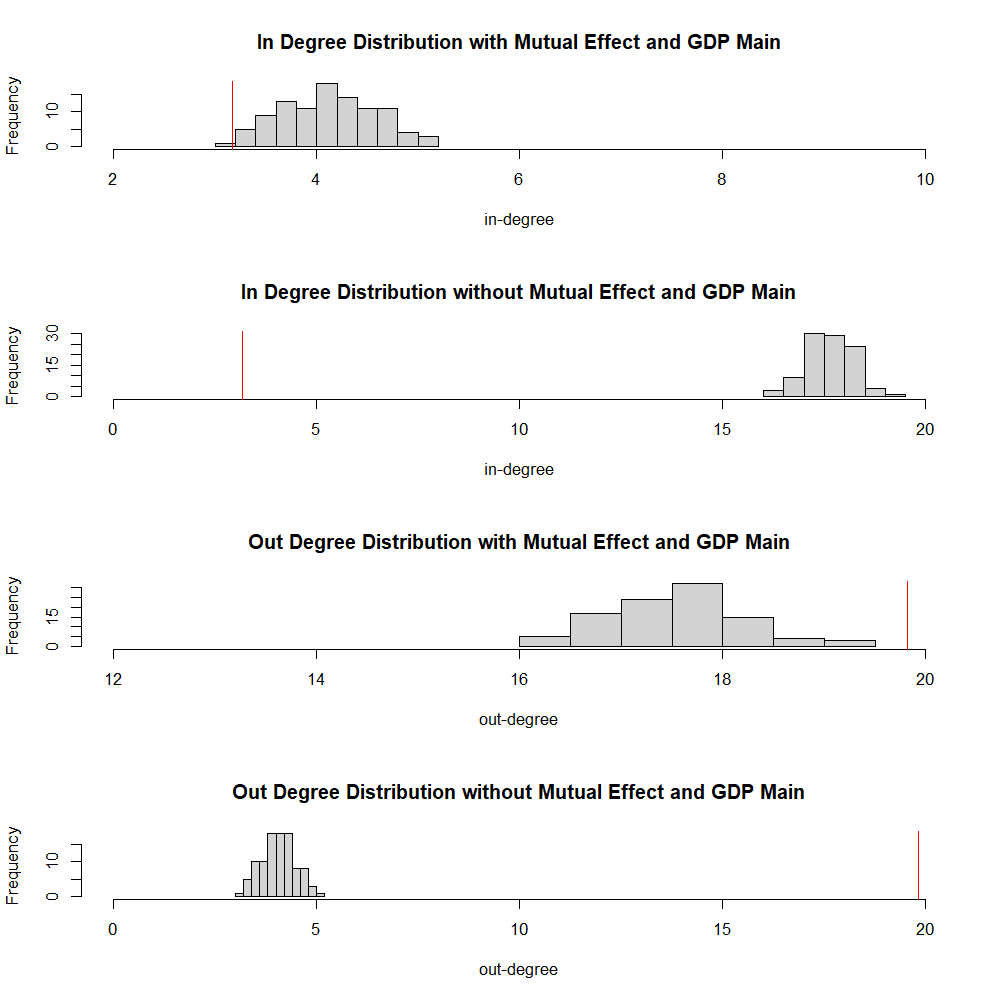
\includegraphics{images/model_SocialCirtcuit_onlyK2Paths_VS_model_SocialCirtcuit_onlyK2Paths_NoMutualEffect_NoGDPMain__Part1.png}

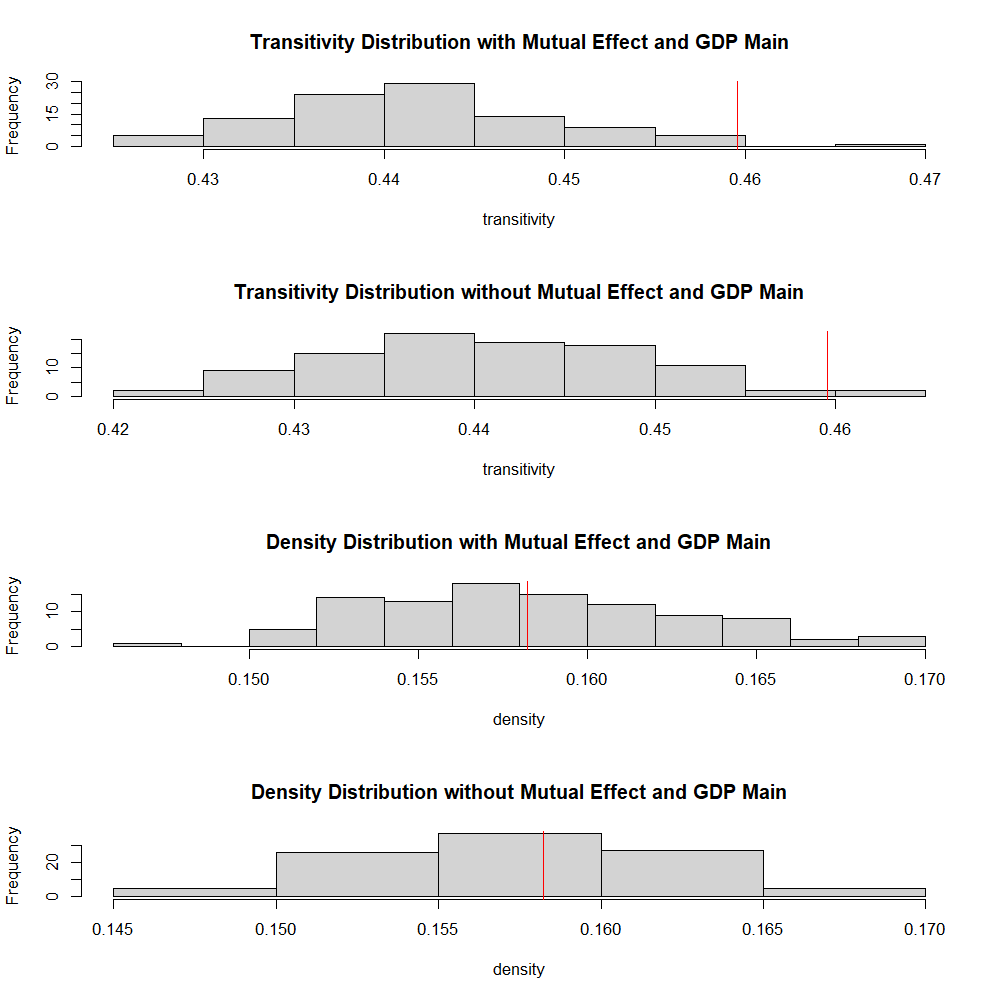
\includegraphics{images/model_SocialCirtcuit_onlyK2Paths_VS_model_SocialCirtcuit_onlyK2Paths_NoMutualEffect_NoGDPMain__Part2.png}

    Anche se secondo il BIC il secondo modello dovrebbe essere leggermente
meglio, prendendo in considerazione anche questi istogrammi ci rendiamo
conto come il primo modello in realtà sia nettamente superiore rispetto
al secondo.

    \subsection{Finite Mixtures}\label{finite-mixtures}

    \subsubsection{Stochastic Block Model}\label{stochastic-block-model}

    Adesso andiamo a calcolare lo Stochastic Block Model per la nostra rete

    \begin{tcolorbox}[breakable, size=fbox, boxrule=1pt, pad at break*=1mm,colback=cellbackground, colframe=cellborder]
\prompt{In}{incolor}{50}{\boxspacing}
\begin{Verbatim}[commandchars=\\\{\}]
\PY{n+nf}{png}\PY{p}{(}\PY{l+s}{\PYZdq{}}\PY{l+s}{images/estimateSBM.png\PYZdq{}}\PY{p}{,}\PY{+w}{ }\PY{n}{width}\PY{+w}{ }\PY{o}{=}\PY{+w}{ }\PY{l+m}{1000}\PY{p}{,}\PY{+w}{ }\PY{n}{height}\PY{+w}{ }\PY{o}{=}\PY{+w}{ }\PY{l+m}{1000}\PY{p}{,}\PY{+w}{ }\PY{n}{res}\PY{+w}{ }\PY{o}{=}\PY{+w}{ }\PY{l+m}{150}\PY{p}{)}
\PY{n}{sbm1}\PY{+w}{ }\PY{o}{\PYZlt{}\PYZhy{}}\PY{+w}{ }\PY{n+nf}{estimateSimpleSBM}\PY{p}{(}\PY{n+nf}{as.matrix}\PY{p}{(}\PY{n}{Y}\PY{p}{)}\PY{p}{,}\PY{+w}{ }\PY{l+s}{\PYZdq{}}\PY{l+s}{bernoulli\PYZdq{}}\PY{p}{,}\PY{+w}{ }\PY{n}{dimLabels}\PY{+w}{ }\PY{o}{=}\PY{+w}{ }\PY{l+s}{\PYZsq{}}\PY{l+s}{nations\PYZsq{}}\PY{p}{,}
\PY{+w}{												 }\PY{n}{estimOptions}\PY{+w}{ }\PY{o}{=}\PY{+w}{ }\PY{n+nf}{list}\PY{p}{(}\PY{n}{verbosity}\PY{+w}{ }\PY{o}{=}\PY{+w}{ }\PY{l+m}{1}\PY{p}{)}\PY{p}{)}
\PY{n+nf}{invisible}\PY{p}{(}\PY{n+nf}{dev.off}\PY{p}{(}\PY{p}{)}\PY{p}{)}
\end{Verbatim}
\end{tcolorbox}

    \begin{Verbatim}[commandchars=\\\{\}]
-> Estimation for 1 groups
-> Computation of eigen decomposition used for initalizations

-> Pass 1
-> Pass 2
-> Pass 3
-> Pass 4
    \end{Verbatim}

    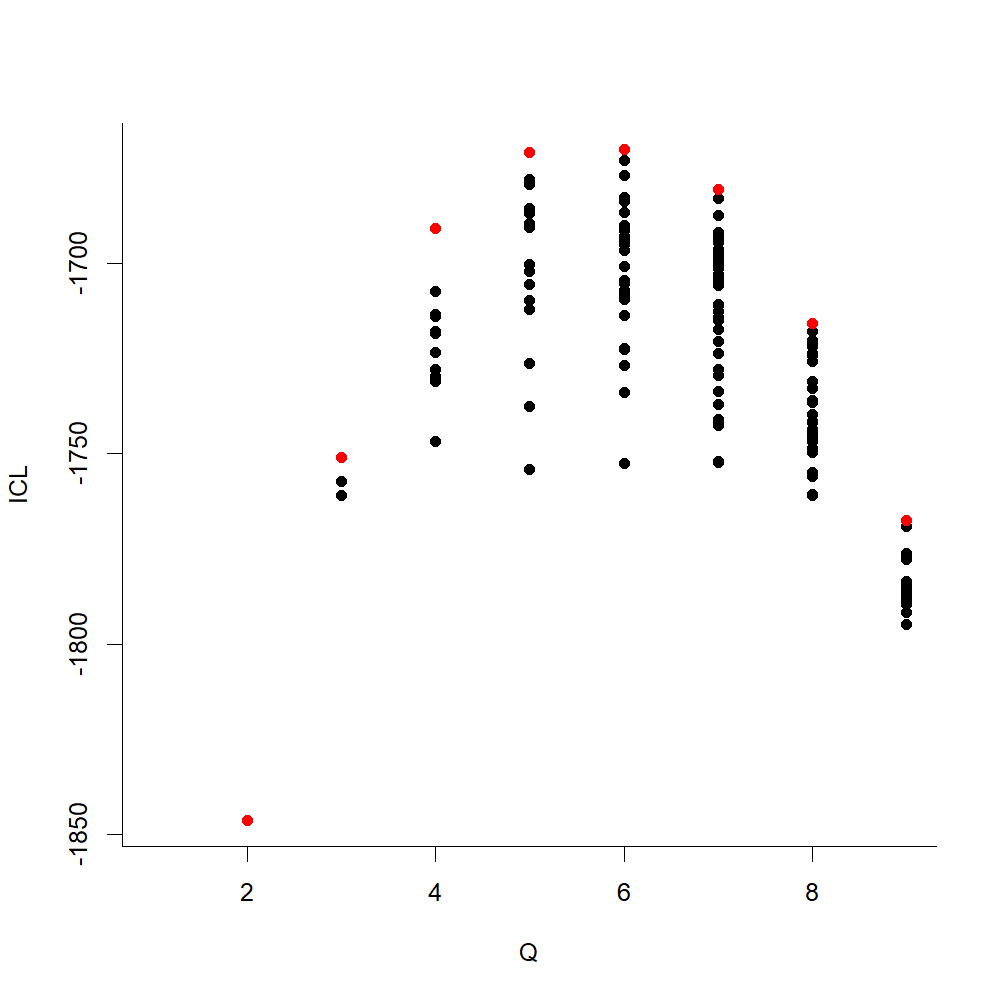
\includegraphics{images/estimateSBM.png}

    A quanto pare il numero migliore di blocchi per la nostra rete è 6 (che
corrisponde al numero di contienti della nostra rete).

    \begin{tcolorbox}[breakable, size=fbox, boxrule=1pt, pad at break*=1mm,colback=cellbackground, colframe=cellborder]
\prompt{In}{incolor}{51}{\boxspacing}
\begin{Verbatim}[commandchars=\\\{\}]
\PY{n}{sbm1}
\end{Verbatim}
\end{tcolorbox}

    
    \begin{Verbatim}[commandchars=\\\{\}]
Fit of a Simple Stochastic Block Model -- bernoulli variant
=====================================================================
Dimension = ( 80 ) - ( 6 ) blocks and no covariate(s).
=====================================================================
* Useful fields 
  \$nbNodes, \$modelName, \$dimLabels, \$nbBlocks, \$nbCovariates, \$nbDyads
  \$blockProp, \$connectParam, \$covarParam, \$covarList, \$covarEffect 
  \$expectation, \$indMemberships, \$memberships 
* R6 and S3 methods 
  \$rNetwork, \$rMemberships, \$rEdges, plot, print, coef 
* Additional fields
  \$probMemberships, \$loglik, \$ICL, \$storedModels, 
* Additional methods 
  predict, fitted, \$setModel, \$reorder 
    \end{Verbatim}

    
    \begin{tcolorbox}[breakable, size=fbox, boxrule=1pt, pad at break*=1mm,colback=cellbackground, colframe=cellborder]
\prompt{In}{incolor}{52}{\boxspacing}
\begin{Verbatim}[commandchars=\\\{\}]
\PY{n}{m}\PY{+w}{ }\PY{o}{\PYZlt{}\PYZhy{}}\PY{+w}{ }\PY{n+nf}{matrix}\PY{p}{(}\PY{n+nf}{round}\PY{p}{(}\PY{n}{sbm1}\PY{o}{\PYZdl{}}\PY{n}{connectParam}\PY{o}{\PYZdl{}}\PY{n}{mean}\PY{p}{,}\PY{+w}{ }\PY{l+m}{3}\PY{p}{)}\PY{p}{,}\PY{+w}{ }\PY{n}{nrow}\PY{+w}{ }\PY{o}{=}\PY{+w}{ }\PY{l+m}{6}\PY{p}{,}\PY{+w}{ }
\PY{+w}{  }\PY{n}{byrow}\PY{+w}{ }\PY{o}{=}\PY{+w}{ }\PY{k+kc}{FALSE}\PY{p}{,}\PY{+w}{ }
\PY{+w}{  }\PY{n}{dimnames}\PY{+w}{ }\PY{o}{=}\PY{+w}{ }\PY{n+nf}{list}\PY{p}{(}\PY{n+nf}{c}\PY{p}{(}\PY{l+s}{\PYZdq{}}\PY{l+s}{B1\PYZdq{}}\PY{p}{,}\PY{+w}{ }\PY{l+s}{\PYZdq{}}\PY{l+s}{B2\PYZdq{}}\PY{p}{,}\PY{+w}{ }\PY{l+s}{\PYZdq{}}\PY{l+s}{B3\PYZdq{}}\PY{p}{,}\PY{+w}{ }\PY{l+s}{\PYZdq{}}\PY{l+s}{B4\PYZdq{}}\PY{p}{,}\PY{+w}{ }\PY{l+s}{\PYZdq{}}\PY{l+s}{B5\PYZdq{}}\PY{p}{,}\PY{+w}{ }\PY{l+s}{\PYZdq{}}\PY{l+s}{B6\PYZdq{}}\PY{p}{)}\PY{p}{,}\PY{+w}{ }\PY{n+nf}{c}\PY{p}{(}\PY{l+s}{\PYZdq{}}\PY{l+s}{B1\PYZdq{}}\PY{p}{,}\PY{+w}{ }\PY{l+s}{\PYZdq{}}\PY{l+s}{B2\PYZdq{}}\PY{p}{,}\PY{+w}{ }\PY{l+s}{\PYZdq{}}\PY{l+s}{B3\PYZdq{}}\PY{p}{,}\PY{+w}{ }\PY{l+s}{\PYZdq{}}\PY{l+s}{B4\PYZdq{}}\PY{p}{,}\PY{+w}{ }\PY{l+s}{\PYZdq{}}\PY{l+s}{B5\PYZdq{}}\PY{p}{,}\PY{+w}{ }\PY{l+s}{\PYZdq{}}\PY{l+s}{B6\PYZdq{}}\PY{p}{)}\PY{p}{)}\PY{p}{)}

\PY{n+nf}{png}\PY{p}{(}\PY{l+s}{\PYZdq{}}\PY{l+s}{images/SBM\PYZus{}HeatMap.png\PYZdq{}}\PY{p}{,}\PY{+w}{ }\PY{n}{width}\PY{+w}{ }\PY{o}{=}\PY{+w}{ }\PY{l+m}{1000}\PY{p}{,}\PY{+w}{ }\PY{n}{height}\PY{+w}{ }\PY{o}{=}\PY{+w}{ }\PY{l+m}{1000}\PY{p}{,}\PY{+w}{ }\PY{n}{res}\PY{+w}{ }\PY{o}{=}\PY{+w}{ }\PY{l+m}{150}\PY{p}{)}

\PY{n+nf}{image}\PY{p}{(}\PY{l+m}{1}\PY{o}{:}\PY{n+nf}{nrow}\PY{p}{(}\PY{n}{m}\PY{p}{)}\PY{p}{,}\PY{+w}{ }\PY{l+m}{1}\PY{o}{:}\PY{n+nf}{ncol}\PY{p}{(}\PY{n}{m}\PY{p}{)}\PY{p}{,}\PY{+w}{ }\PY{n+nf}{t}\PY{p}{(}\PY{n+nf}{apply}\PY{p}{(}\PY{n}{m}\PY{p}{,}\PY{+w}{ }\PY{l+m}{2}\PY{p}{,}\PY{+w}{ }\PY{n}{rev}\PY{p}{)}\PY{p}{)}\PY{p}{,}\PY{+w}{ }\PY{n}{axes}\PY{+w}{ }\PY{o}{=}\PY{+w}{ }\PY{k+kc}{FALSE}\PY{p}{,}\PY{+w}{ }\PY{n}{main}\PY{+w}{ }\PY{o}{=}\PY{+w}{ }\PY{l+s}{\PYZdq{}}\PY{l+s}{Matrix Heatmap of SBM\PYZdq{}}\PY{p}{,}\PY{+w}{ }\PY{n}{xlab}\PY{+w}{ }\PY{o}{=}\PY{+w}{ }\PY{l+s}{\PYZdq{}}\PY{l+s}{\PYZdq{}}\PY{p}{,}\PY{+w}{ }\PY{n}{ylab}\PY{+w}{ }\PY{o}{=}\PY{+w}{ }\PY{l+s}{\PYZdq{}}\PY{l+s}{\PYZdq{}}\PY{p}{,}\PY{+w}{ }\PY{n}{zlim}\PY{+w}{ }\PY{o}{=}\PY{+w}{ }\PY{n+nf}{c}\PY{p}{(}\PY{l+m}{0}\PY{p}{,}\PY{+w}{ }\PY{l+m}{1}\PY{p}{)}\PY{p}{)}

\PY{n+nf}{for}\PY{p}{(}\PY{n}{i}\PY{+w}{ }\PY{n}{in}\PY{+w}{ }\PY{l+m}{1}\PY{o}{:}\PY{n+nf}{nrow}\PY{p}{(}\PY{n}{m}\PY{p}{)}\PY{p}{)}\PY{+w}{ }\PY{p}{\PYZob{}}
\PY{+w}{  }\PY{n+nf}{for}\PY{p}{(}\PY{n}{j}\PY{+w}{ }\PY{n}{in}\PY{+w}{ }\PY{l+m}{1}\PY{o}{:}\PY{n+nf}{ncol}\PY{p}{(}\PY{n}{m}\PY{p}{)}\PY{p}{)}\PY{+w}{ }\PY{p}{\PYZob{}}
\PY{+w}{    }\PY{n+nf}{text}\PY{p}{(}\PY{n}{i}\PY{p}{,}\PY{+w}{ }\PY{n+nf}{ncol}\PY{p}{(}\PY{n}{m}\PY{p}{)}\PY{o}{\PYZhy{}}\PY{n}{j}\PY{l+m}{+1}\PY{p}{,}\PY{+w}{ }\PY{n}{labels}\PY{+w}{ }\PY{o}{=}\PY{+w}{ }\PY{n+nf}{t}\PY{p}{(}\PY{n}{m}\PY{p}{)}\PY{p}{[}\PY{n}{i}\PY{p}{,}\PY{n}{j}\PY{p}{]}\PY{p}{,}\PY{+w}{ }\PY{n}{cex}\PY{+w}{ }\PY{o}{=}\PY{+w}{ }\PY{l+m}{1.2}\PY{p}{)}
\PY{+w}{  }\PY{p}{\PYZcb{}}
\PY{p}{\PYZcb{}}

\PY{n+nf}{mtext}\PY{p}{(}\PY{n+nf}{rownames}\PY{p}{(}\PY{n}{m}\PY{p}{)}\PY{p}{,}\PY{+w}{ }\PY{n}{side}\PY{+w}{ }\PY{o}{=}\PY{+w}{ }\PY{l+m}{3}\PY{p}{,}\PY{+w}{ }\PY{n}{at}\PY{+w}{ }\PY{o}{=}\PY{+w}{ }\PY{l+m}{1}\PY{o}{:}\PY{n+nf}{nrow}\PY{p}{(}\PY{n}{m}\PY{p}{)}\PY{p}{,}\PY{+w}{ }\PY{n}{line}\PY{+w}{ }\PY{o}{=}\PY{+w}{ }\PY{l+m}{0.2}\PY{p}{)}
\PY{n+nf}{mtext}\PY{p}{(}\PY{n+nf}{rev}\PY{p}{(}\PY{n+nf}{colnames}\PY{p}{(}\PY{n}{m}\PY{p}{)}\PY{p}{)}\PY{p}{,}\PY{+w}{ }\PY{n}{side}\PY{+w}{ }\PY{o}{=}\PY{+w}{ }\PY{l+m}{2}\PY{p}{,}\PY{+w}{ }\PY{n}{at}\PY{+w}{ }\PY{o}{=}\PY{+w}{ }\PY{l+m}{1}\PY{o}{:}\PY{n+nf}{ncol}\PY{p}{(}\PY{n}{m}\PY{p}{)}\PY{p}{,}\PY{+w}{ }\PY{n}{line}\PY{+w}{ }\PY{o}{=}\PY{+w}{ }\PY{l+m}{0.2}\PY{p}{)}

\PY{n+nf}{invisible}\PY{p}{(}\PY{n+nf}{dev.off}\PY{p}{(}\PY{p}{)}\PY{p}{)}
\end{Verbatim}
\end{tcolorbox}

    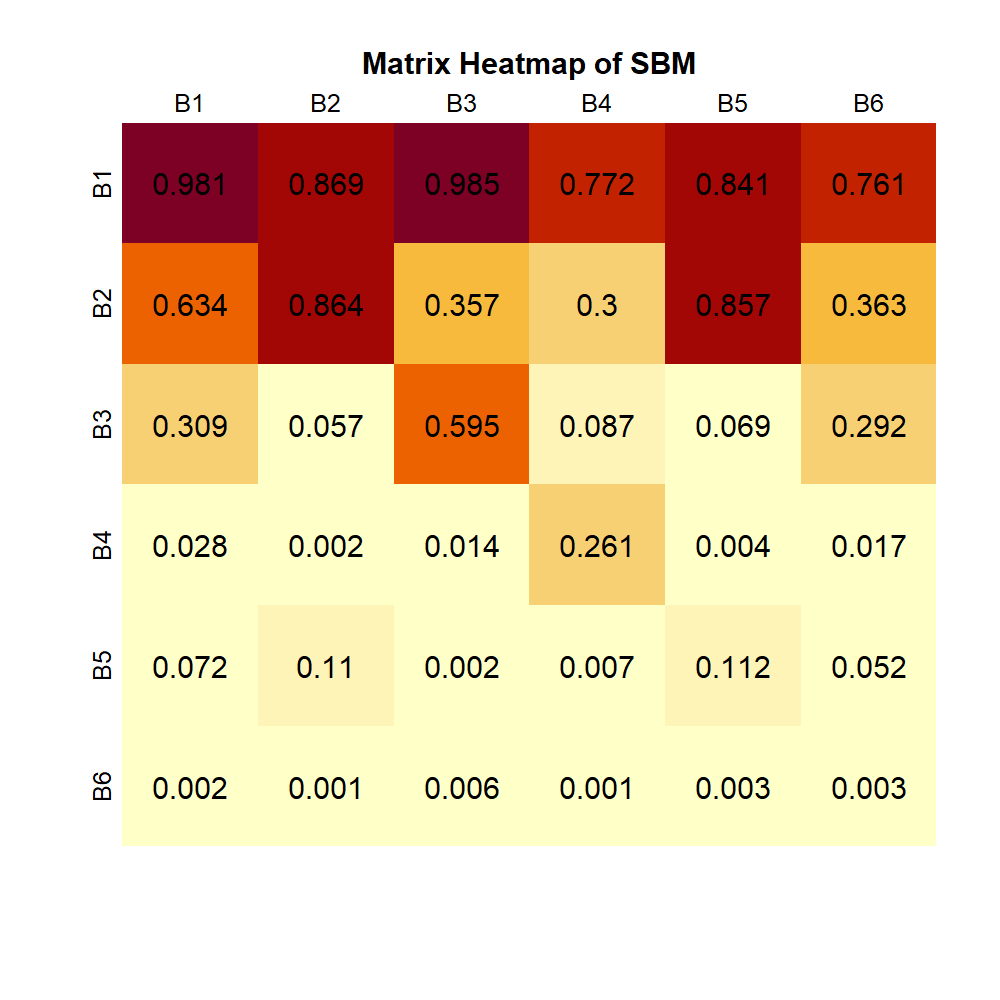
\includegraphics{images/SBM_HeatMap.png}

    Analizzando l'Heatmap possiamo dedurre che:

\begin{itemize}
\tightlist
\item
  Il Blocco 1, composto da Paesi molto sviluppati (come Germania, Italia
  e Stati Uniti), invia collegamenti a tutti, specialmente a sé stesso,
  al Blocco 3 e al Blocco 5.
\item
  Il Blocco 2, composto solamente da Paesi europei, invia collegamenti a
  tutti, anche se in minore quantità rispetto al Blocco 1, specialmente
  con sé stesso e il Blocco 5.
\item
  Il Blocco 3, composto solamente da Paesi asiatici, invia collegamenti
  principalmente a sé stesso e in minore quantità anche con il Blocco 1
  e il Blocco 6.
\item
  Il Blocco 4, composto solamente da Paesi Americani, invia pochi
  collegamenti e principalmente a sé stesso.
\item
  Il Blocco 5, composto solamente da Paesi europei, invia pochissimi
  collegamenti e principalmente a sé stesso, il Blocco 1 e il Blocco 6
\item
  Il Blocco 6, composto dai Paesi rimanenti (principlamente poco
  sviluppati), invia quasi nessun collegamento.
\end{itemize}

    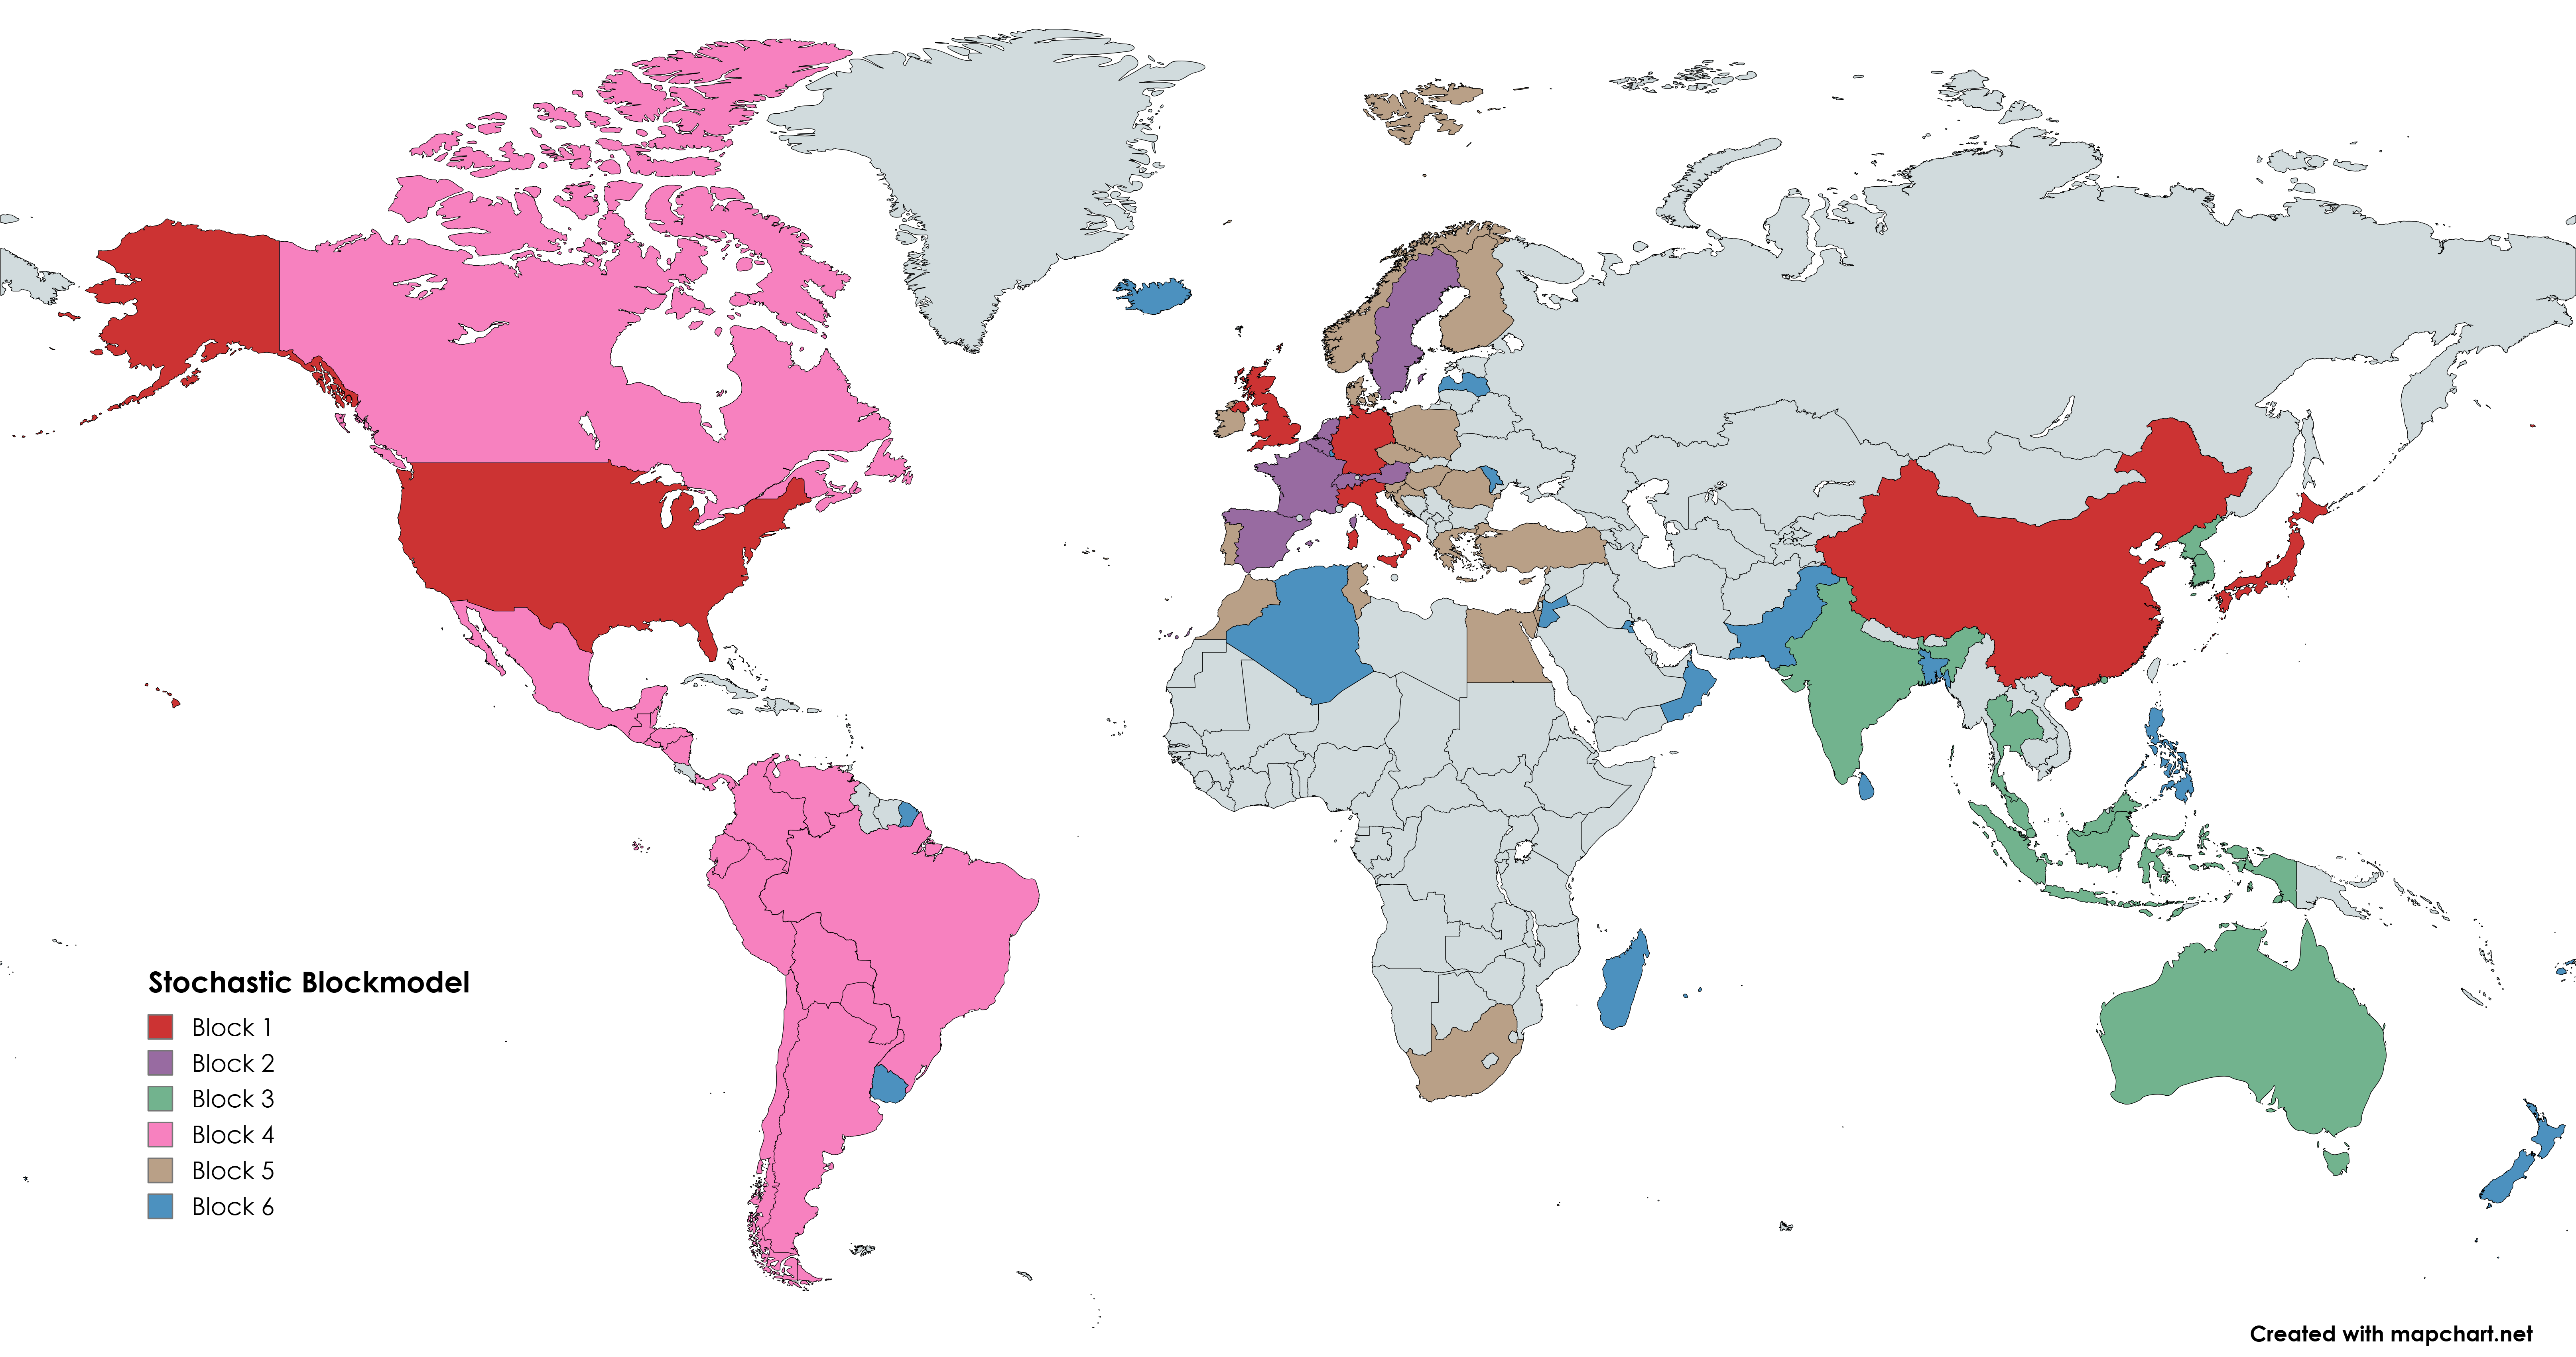
\includegraphics{imagesWorldMaps/Stochastic_Blockmodel.png}

Divisione degli 80 Paesi in base ai Blocchi del SBM

    \section{Conclusioni}\label{conclusioni}

    Alla fine possiamo trarre la conclusione che esiste una correlazione
significativa tra lo scambio di metalli e la ricchezza di un paese.
Questo fenomeno può essere attribuito al fatto che nei Paesi più
sviluppati economicamente, il costo della manodopera è generalmente più
elevato rispetto ai Paesi meno sviluppati. Inoltre, i metalli sono
spesso utilizzati come materie prime per l'industria manifatturiera e
l'edilizia, settori strettamente legati alla crescita economica. Di
conseguenza, risulta più conveniente per i Paesi più ricchi importare i
metalli piuttosto che estrarli autonomamente. Tuttavia, è importante
sottolineare che ulteriori ricerche e analisi sono necessarie per
approfondire la natura di questa relazione e comprendere appieno i
fattori che la influenzano.


    % Add a bibliography block to the postdoc
    
    
    
\end{document}
